%!TEX TS-program = xelatex
%!TEX encoding = UTF-8 Unicode

\documentclass{Dissertate}

\listfiles

\begin{document}

\def\bibfont{\small}
\renewcommand\refname{}

%%%% FIRST PAGES %%%%%%%%%%%%	

%!TEX root = ../thesis.tex

\chapter*{}

\pagenumbering{gobble}

\begin{tikzpicture}[remember picture,overlay]
\node at (current page.center) {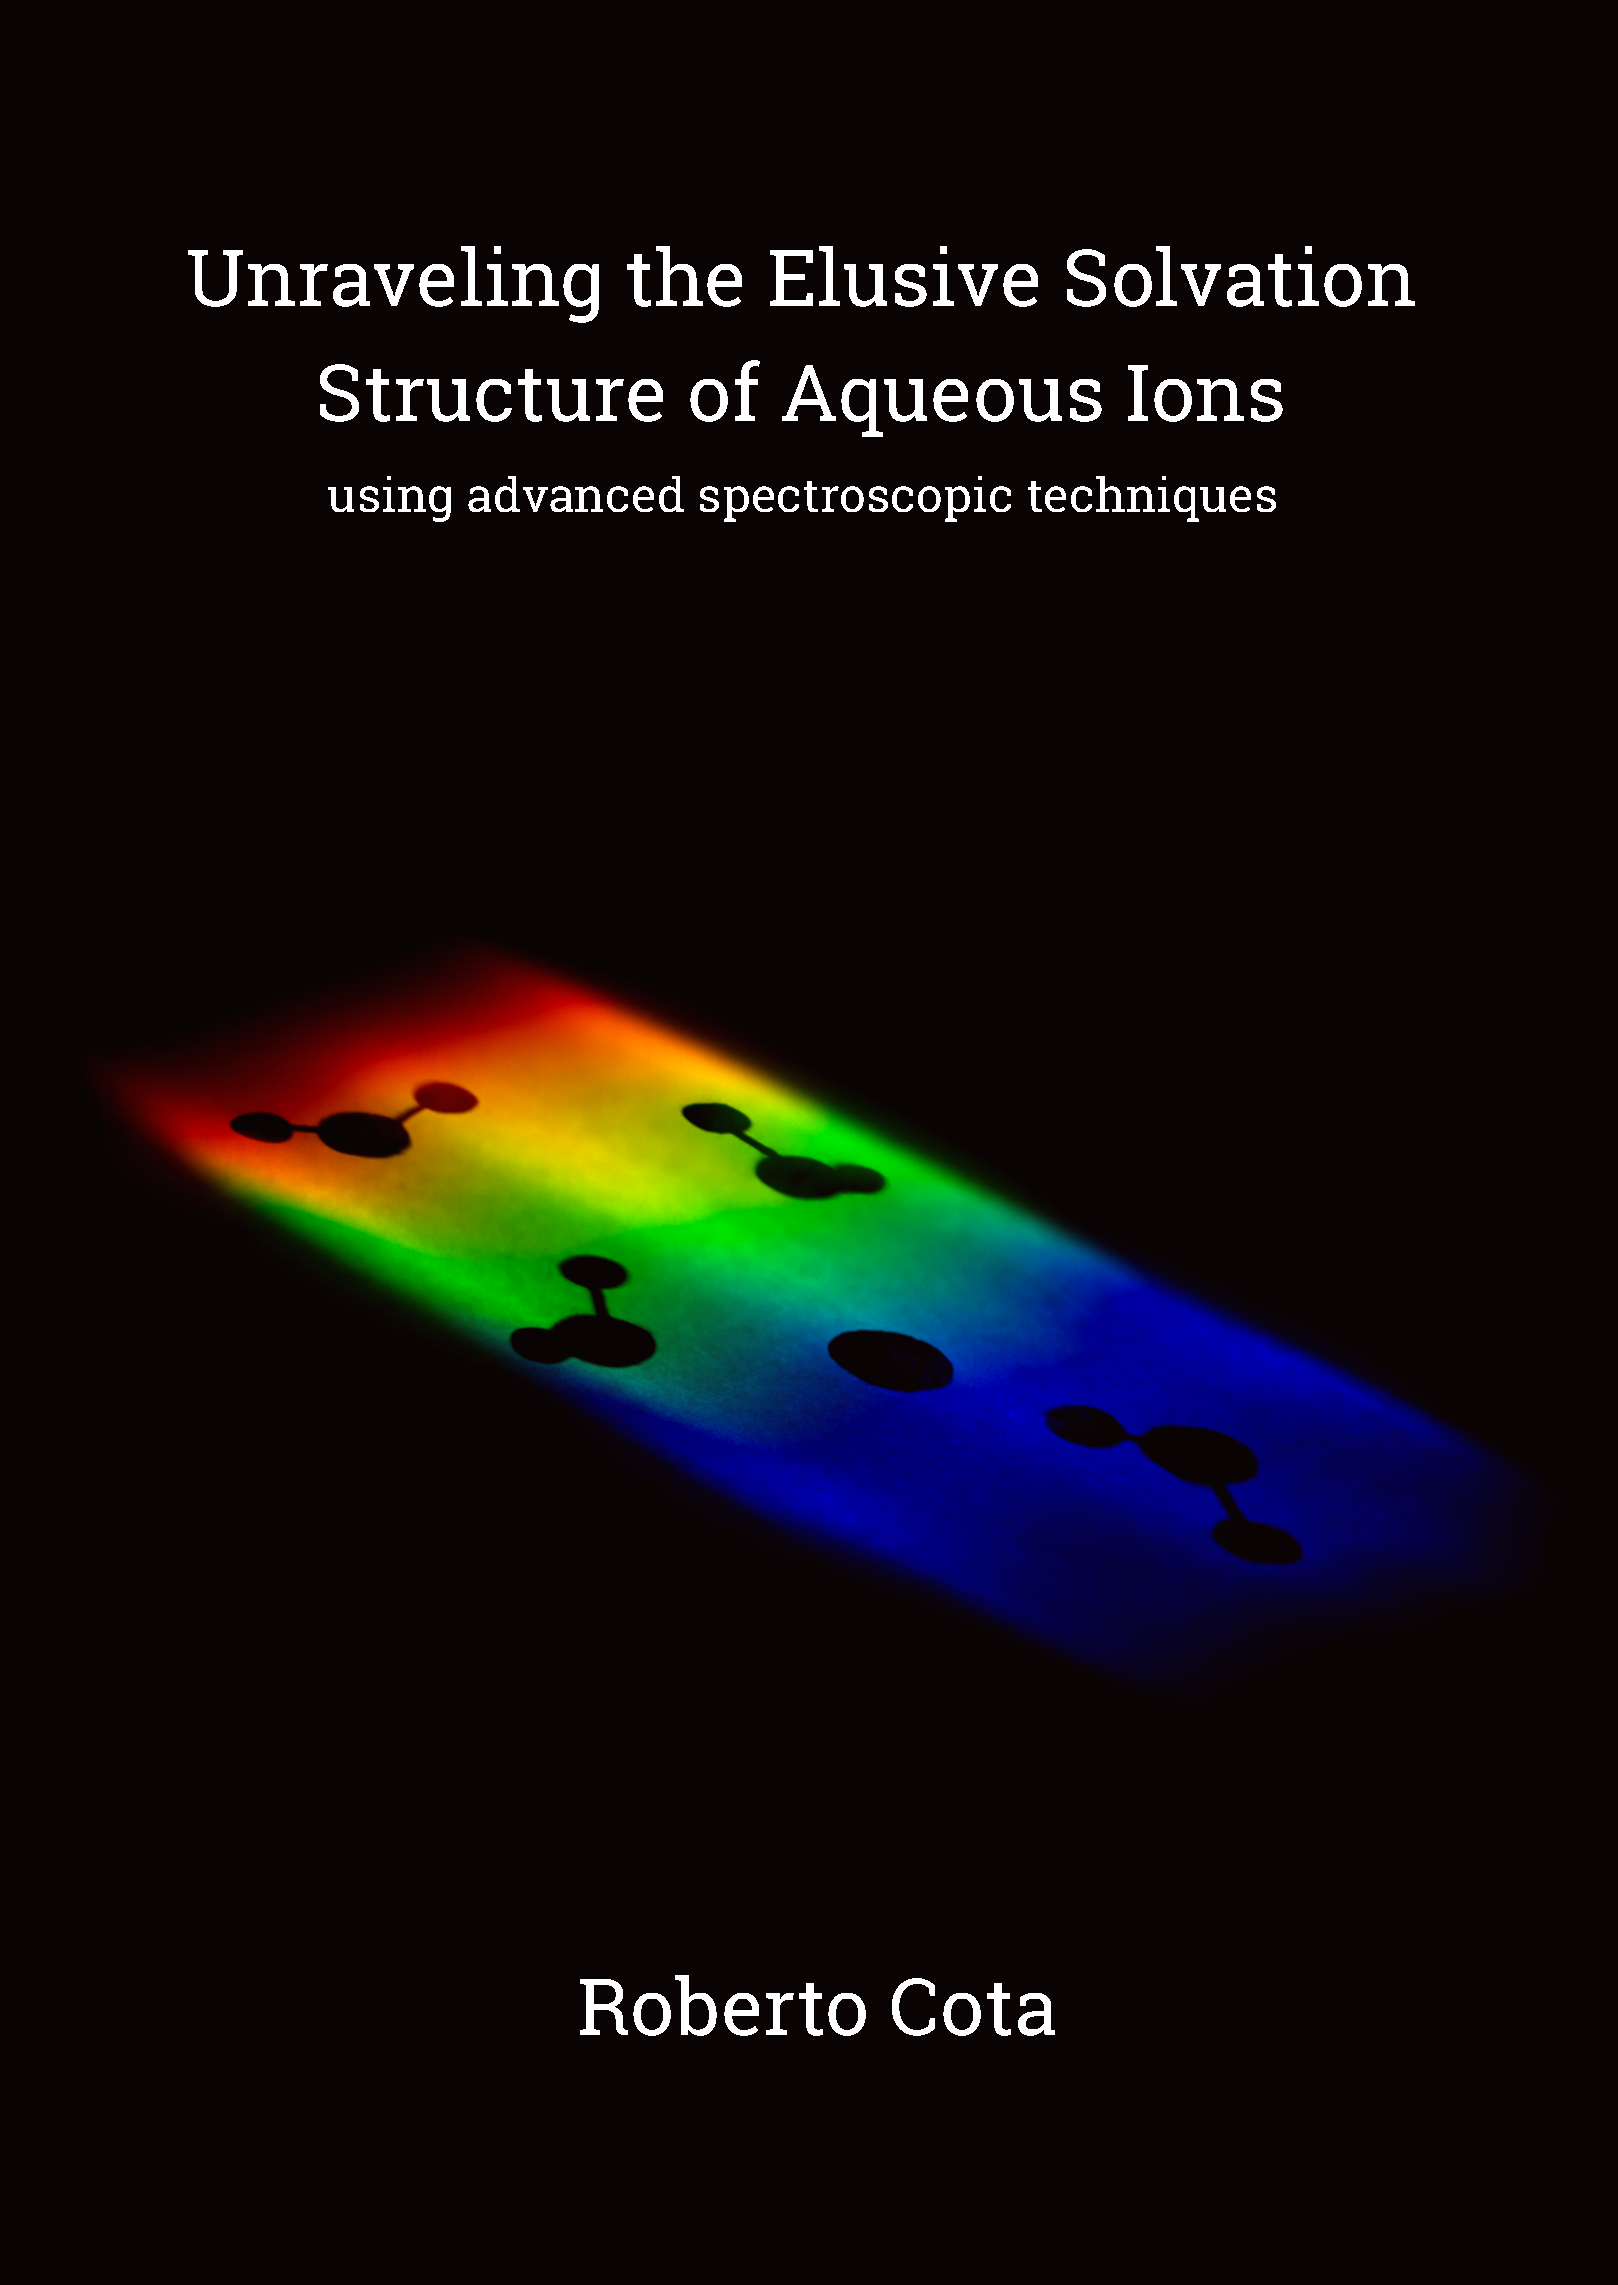
\includegraphics[width=\pdfpagewidth,height=\pdfpageheight]{fullpage_images/Cover4Digital.pdf}};
\end{tikzpicture}

% Add personal and university information
%!TEX root = ../thesis.tex


\newcommand{\bigsizes}{\fontsize{17pt}{20pt}\selectfont}
\newcommand{\Namesize}{\fontsize{13pt}{20pt}\selectfont}
\newcommand{\Titulosize}{\fontsize{13pt}{20pt}\selectfont}

\chapter*{}
\pagenumbering{Roman}
\setcounter{page}{1}
\thispagestyle{empty}






%\vspace*{\fill}
\vspace{13pt}
\begin{center}
	{\bfseries\bigsizes\color{SchoolColor} Unraveling the elusive solvation structure of aqueous ions using advanced spectroscopic techniques} \normalsize \\
	%	\Huge \textcolor{blue}{\thetitle} \normalsize \\
\end{center}

\vspace{9.0cm}
	
\begin{center}	
{\bfseries\Namesize Roberto Oziel Gutierrez Cota}
\end{center}
\vspace*{\fill}




\newpage
\thispagestyle{empty}

\vspace*{\fill}
\vspace{10cm}

\noindent Cover image: artistic picture of a spectroscopic experiment in which \\molecules are indirectly observed through the shadows that they cast.

\medskip

\noindent Designed by Kateryna Kulakova \& Roberto Cota

\vspace{0.6cm}

\noindent ISBN: 978-94-028-1999-1

\vspace{0.6cm}

\noindent Digital version of this thesis is available at 
\href{https://dare.uva.nl}{https://dare.uva.nl} 

\vspace{0.6cm}

\noindent Printed and bound by Ipskamp Printing B.V.

\vspace{0.6cm}

\noindent Amsterdam, Netherlands, 2020


\vspace*{\fill}



\chapter*{} %Empty page



\vspace*{\fill}
\vspace{-65pt}
\begin{center}
	{\bfseries\bigsizes\color{SchoolColor} Unraveling the elusive solvation structure of aqueous ions using advanced spectroscopic techniques} \normalsize \\
	%	\Huge \textcolor{blue}{\thetitle} \normalsize \\
	\vspace{40pt}
	
{\Namesize ACADEMISCH PROEFSCHRIFT}

\vspace{40pt}
	
ter verkrijging van de graad van doctor

\vspace{5pt}

aan de Universiteit van Amsterdam

\vspace{5pt}
	
op gezag van de Rector Magnificus

\vspace{5pt}
	
prof. dr. ir. K.I.J. Maex

\vspace{5pt}
	
ten overstaan van een door het College voor Promoties ingestelde commissie,

\vspace{5pt}

in het openbaar te verdedigen in de Aula der Universiteit

\vspace{15pt}

op vrijdag 30 oktober 2020, te 11:00 uur

	\vspace{25pt}

door 

	\vspace{25pt}
	
	
{\bfseries\Namesize Roberto Oziel Gutierrez Cota}

	\vspace{25pt}

geboren te Leon
\end{center}
\vspace*{\fill}

\thispagestyle{empty}
\newpage
%\thispagestyle{empty}






\begin{flushleft}
{\bfseries\large Promotiecommissie:}

\vspace{20pt}

\noindent \makebox[2.8cm][l]{Promotoren:} \makebox[4.3cm][l]{Prof. dr. S. Woutersen} Universiteit van Amsterdam

\vspace{5pt}

\noindent \makebox[2.8cm][l]{} \makebox[4.3cm][l]{Prof. dr. H. J. Bakker} Universiteit van Amsterdam

\vspace{20pt}


\noindent \makebox[2.8cm][l]{Overige leden:} \makebox[4.3cm][l]{Prof. dr. R. Buchner} Universit\"at Regensburg

\vspace{5pt}

\noindent \makebox[2.8cm][l]{} \makebox[4.3cm][l]{Prof. dr. E. H. G. Backus} Universit\"at Wien

\vspace{5pt}

\noindent \makebox[2.8cm][l]{} \makebox[4.3cm][l]{Prof. dr. W. J. Buma} Universiteit van Amsterdam

\vspace{5pt}

\noindent \makebox[2.8cm][l]{} \makebox[4.3cm][l]{Prof. dr. E. J. Meijer} Universiteit van Amsterdam

\vspace{5pt}

\noindent \makebox[2.8cm][l]{} \makebox[4.3cm][l]{Dr. B. Ensing} Universiteit van Amsterdam





\vspace{20pt}

\makebox[2.8cm][l]{Faculteit:} Faculteit der Natuurwetenschappen, Wiskunde en Informatica


\end{flushleft}

\vspace{5.5cm}



\begin{figure}[h!]
	\centering
	
\includegraphics[width=0.95\textwidth]{frontmatter/AllLogos.png}
\end{figure}

\vspace{0.5cm}

\noindent The research covered in this thesis was conducted in the Molecular Photonic Group at the Van 't Hoff Institute for Molecular Sciences, University of Amsterdam, and the Ultrafast Spectroscopy Group at AMOLF, Amsterdam. This work was financially supported by the Netherlands Organisation for Scientific Research (NWO). Grant number: 12PR2989.


\vspace*{\fill}



\setstretch{\dnormalspacing}

% Add dedication (or not)
\dedicationpage{frontmatter/dedication}

% Publications 
% Add publication list: this command has been defined
% in the dissertate class
%!TEX root = ../thesis.tex

\chapter*{}
\publicationspage

% Add table of contents
\tableofcontents


%%%%%%%%%			CHAPTERS		%%%%%%%%%%

% First chapter image
% Add an empty page if the table of contents finishes in 
% a even number, otherwise comment the next line
%!TEX root = ../thesis.tex

\chapter*{}

\thispagestyle{empty}
\begin{tikzpicture}[remember picture,overlay]
	\node at (current page.center) {
\includegraphics[width=1\pdfpagewidth,height=1\pdfpageheight]{fullpage_images/stereoFinalePDF.pdf}};
\end{tikzpicture}
% If no image is desired, comment all this block
% Note: for the second chapter and upwards these lines
% are defined inside the chapter*.tex file



\onehalfspacing
\mainmatter
\pagestyle{fancy}
\renewcommand{\chaptermark}[1]{\markboth{#1}{#1}}
\renewcommand{\sectionmark}[1]{\markright{\thesection\ #1}}
\lhead[\fancyplain{}]{{\nouppercase\rightmark}}
\rhead[\fancyplain{}{\nouppercase\leftmark}]{}

\begin{spacing}{\dcompressedspacing}


%%% ADD CHAPTERS

%!TEX root = ../thesis.tex

\begin{savequote}[75mm]
$\blacktriangleleft$ I faced the challenge of observing molecules with the help of state-of-the-art experimental techniques. Here, the reader must perform one last experiment using, by far, the most advanced observation instrument that we have: the human eye.

\vspace{3pt}

(Hint: watch it horizontally)
\end{savequote}


\chapter{Introduction}\label{chap:introduction}


\vspace{30pt}


\section{Water: a structured material}


Despite being the most familiar and abundant compound on earth, water has captivated humankind for centuries. Since ancient times, for example, humans have wondered at the property of ice to float on liquid water, which is the consequence of water having a lower density as a solid than as a liquid. This anomalous behavior finds its origin in the nature of water to form structures: crystal-like networks that increase the volume of the system when it freezes. This example belongs to a long list of anomalies as compared to other liquids,\!\cite{Russo2018} many of which are linked to the structured character of water. However, in spite of considerable efforts, a precise description of its structural properties remains elusive to date.\!\cite{Ball2008}




In liquid water, hydrogen bonds are considered the intermolecular ``glue'' that gives rise to the structure called the hydrogen-bond network. In this network, each hydrogen bond results from the (mainly electrostatic) bonding between one of the partially positive hydrogen atoms and one of the lone-pair electrons in neighboring water molecules. Thus, each water molecule has the potential to participate in the formation of four hydrogen bonds: donating two (two hydrogen atoms) and accepting two (two lone-pair electrons), as depicted in Figure \ref{MoleculeHStructure}. As was validated in 1933 using X-rays, the perfect arrangement of water molecules leads to a periodic tetrahedral structure.\!\cite{Bernal1933}



Recent studies show, however, that liquid water possesses on average 3.5 hydrogen bonds per molecule in ambient conditions.\!\cite{Soper2000,Wernet2004,Kumar2007} This means that the hydrogen-bond network is defective to the extent that it allows changes in the local coordinates as well as structural rearrangements, which have been observed to occur on a sub-picosecond ($\leq$$10^{-12}$~s) time scale.\!\cite{Lawrence2003,Eaves2005,Fecko2005,Laage2006} As such, the hydrogen-bond network of water is a highly active and adaptive environment. It is thus not surprising that many chemical and biological processes occur in aqueous environments---an excellent environment for life to prosper in.\!\cite{Ball2008c,Bellissent-Funel2016,Ball2017}


\begin{figure}[t!]
	\centering
	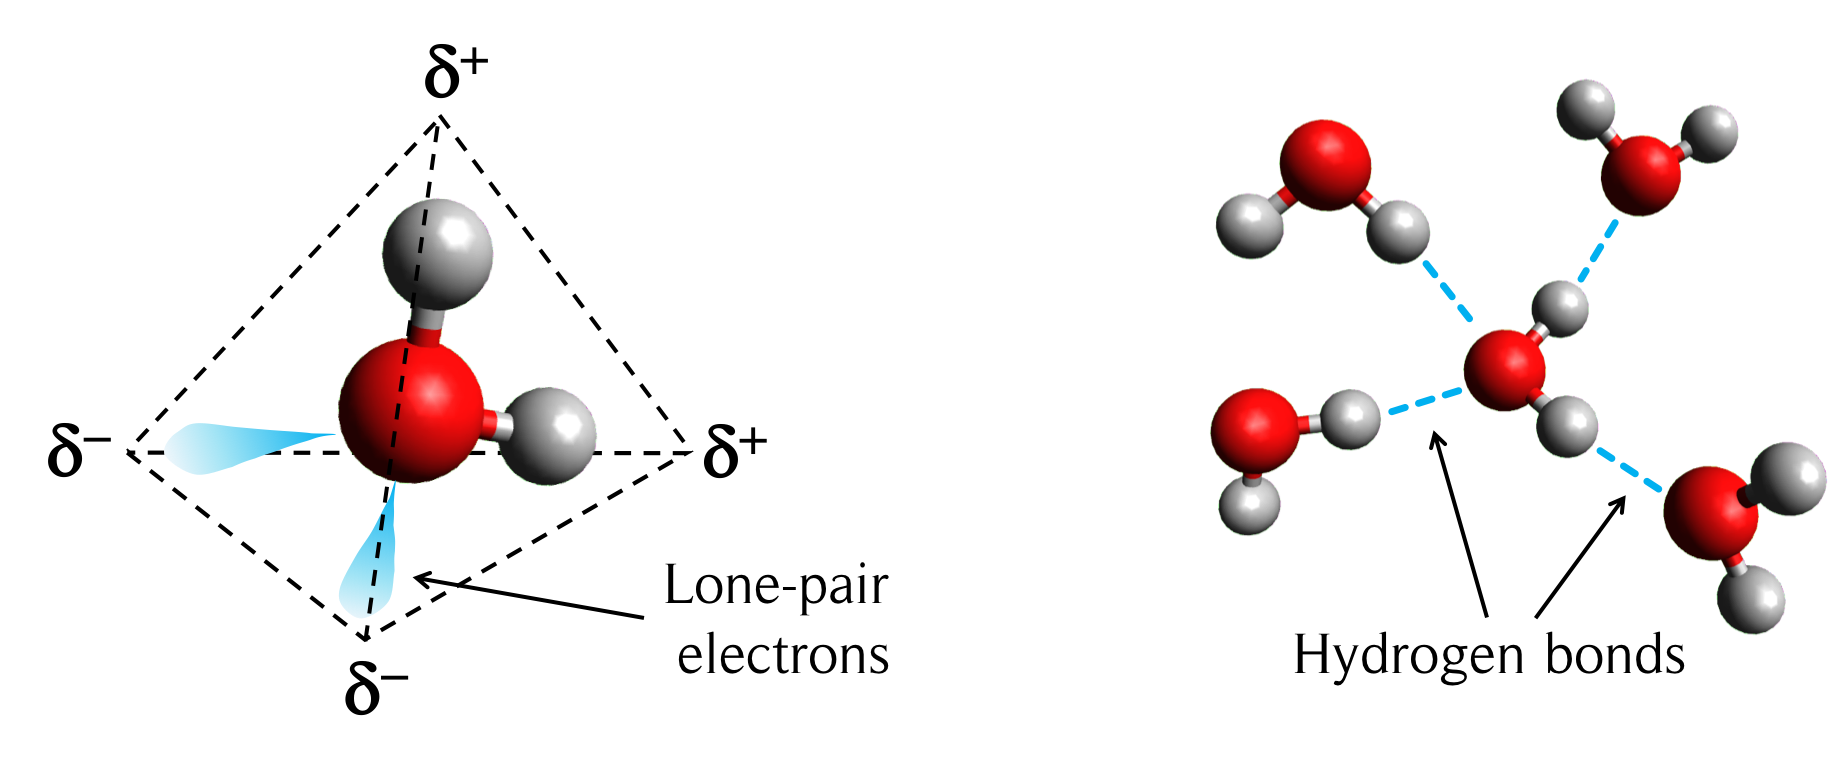
\includegraphics[width=0.8\figwidth]{chapters/Chapter1_Introduction/Graphs/HydrogenBondsC.png} %The local modes are calculated on the XXX level, and reproduced with permission from ref. XXX. 
	\caption{\textbf{Left:} Tetrahedral configuration of a water molecule. \textbf{Right:} Local hydrogen-bond structure of a water molecule that extends to form the so-called hydrogen-bond network of liquid water. }
	\label{MoleculeHStructure}
\end{figure}



Yet, water is often regarded as a stiff liquid, a concept introduced by Marcus,\!\cite{Marcus2009,Marcus2010} in which the hydrogen bonding leads to cooperative dynamics. This cooperativity constrains the mobility of water molecules themselves, as well as the dynamics of other molecules dissolved in water. In aqueous solutions, the solutes can reciprocally affect the cooperative behavior due to discontinuities and defects in the hydrogen-bond network of water. If the concentration of solutes in water is high enough, one can observe changes in the macroscopic properties of water: the viscosity and surface tension increases or decreases depending on the nature of the solute.



\section{The influence of ions on the structure of water}



The way in which ions, among other solutes, modify the structural dynamics of water has been a long-standing question and is an active field of experimental and theoretical research. An accurate description of ion-water interactions is of importance for the study of many chemical and biological processes, ranging from the conformation of proteins to the selection rules for ion exchange in living cells.



In electrolyte solutions, ions generate strong local electric fields that modify the hydrogen-bond structure and induce local molecular ordering in the form of solvation shells. Based on the degree of water structuring in solvation shells, ions are classified as structure makers or structure breakers, concepts coined by Gurney in the 50s.\!\cite{Gurney1953} In this context, while small ions with high surface charge densities are structure makers that form tight solvation shells, large ions form labile solvation structures due to their low surface charge density. 


Most of the work that has been carried out to study ion-water interactions has been reviewed by Yizhak Marcus\!\cite{Marcus1988,Marcus2009} and Hitoshi Ohtaki\!\cite{Ohtaki1993} in three publications that have become a benchmark for the field of solvation. The evolution of the different techniques and their accuracy is observed in these publications. However, the spread in the reviews' results from the different techniques show that a precise description of solvation shells is still lacking.





These discrepancies find their origin in the fact that each technique is sensitive to different time scales and spatial ranges. For instance, scattering methods like X-ray and neutron diffraction deliver static snapshots of ionic structures. These techniques can be used to determine the packing capacity of water molecules around ions; a quantity referred to as \textit{coordination number}. Large ions have large coordination numbers which do not reflect the strength of the solvation interactions, nor dynamic properties such as the residence time of water molecules in solvation shells.


\begin{figure}[t!]
	\centering
	\includegraphics[width=1.0\figwidth]{chapters/Chapter1_Introduction/Graphs/SolvationWater2Aff.pdf} %The local modes are calculated on the XXX level, and reproduced with permission from ref. XXX. 
	\caption{Visual representation of ions dissolved in water, and of ion--water solvation interactions. The strong local electric field of ions induce local ordering in the form of solvation shells. The structural dynamics of solvating water molecules differ from that of water molecules in neat bulk water. As such, the hydrogen-bond network is said to be locally broken.}
	\label{SolvationWaterSchematic}
\end{figure}


In contrast, the hydration number is a wider concept that represents the capacity of ions to bind water molecules long enough that they diffuse with the ion as a whole. Hydration numbers are phenomenologically represented with the Hofmeister series, which follows the surface charge density of the ions under study, i.e.\ $\ce{Li+} > \ce{Na+} > \ce{K+} > \ce{Cs+}$. This explains why $\ce{Cs+}$, which is weakly hydrated, diffuses faster through water than the strongly hydrated $\ce{Na+}$ ion.\!\cite{Cota2018} A straightforward method to determine hydration numbers is based on ionic mobility: from the diffusion coefficients one can determine the effective Stokes radii of ions.\!\cite{Atkins2010} This method intrinsically incorporates dynamic properties, however, ions (with their solvation structures) are considered to be perfect spheres immersed in a uniform continuum (as depicted in Figure \ref{SolvationWaterSchematic}), which is not entirely valid due to the local disruption of the hydrogen-bond network. Another problem in many experiments is the difficulty of separating the corresponding contributions of the cation and of the anion.


From the previous examples, one can deduce that in order to accurately estimate hydration numbers we require experimental techniques that directly measure the influence of ions on the structural dynamics of water. This calls for the adoption of techniques with a (sub)picosecond temporal resolution (the time scale of the structural fluctuations of water), and a method to separate the contributions of cations and anions.











\section{Towards a better understanding of ion solvation}

Over the last 20 years, the experimental situation has substantially improved with the advent of (i) vector network analyzers (VNA) with high (GHz) frequencies; and (ii) femtosecond laser pulses. Both instruments have the ability to retrieve data with high temporal resolution, which has been successfully exploited to study molecular dynamics.\!\cite{Woutersen1999,Buchner2004,Loparo2004,Eaves2005,Logsdon2005,Rezus2005,Fecko2005,Rezus2006,Buchner2008,Thogersen2008,Piatkowski2009,Prajapati2010,Timmer2010,Vyas2011,Rahman2012,Ensing2013,Ermilova2014,Ottosson2014c,Balos2015a,Baiz2015,Stevenson2015,Shattuck2016,Zhang2016,Balos2017a,Strudwick2018}




In particular, information on solvating structures and the dynamics of the hydrogen-bond network is obtained from the reorientation dynamics of water molecules,\!\cite{Buchner2004,Loparo2004,Rezus2005,Rezus2006,Buchner2008,Thogersen2008,Ensing2013,Ottosson2014c,Shattuck2016} a property which is the cornerstone of this thesis.




\subsection{Macroscopic observation of the collective behavior of water}



VNA-based dielectric relaxation spectroscopy (DRS) has been used to explore the structure and dynamics of polar molecules.\!\cite{Buchner2004,Logsdon2005,Buchner2008,Prajapati2010,Vyas2011,Rahman2012,Ensing2013,Ermilova2014,Ottosson2014c,Balos2015a,Balos2017a} From DRS measurements, the dielectric constant defines the magnitude of the polarization that results from the reorientation of dipolar molecules in an applied electric field. In liquid water, the dielectric constant reflects the overall molecular dynamics, which incorporate the cooperative behavior of the hydrogen-bond network. As such, in electrolyte solutions, changes in the dielectric constant can be attributed to variations in the microscopic structure of water, e.g.\ the disruption of the hydrogen-bond network of water and the local molecular ordering in the form of solvation shells.



This technique has the advantage of being primarily sensitive to solvation shells of positive ions. Cations restrict hydrating water molecules to rotations around their main symmetry axis, in which their permanent dipole moments are said to be rotationally immobilized. In contrast, around anions, the dipole moment of hydrating water molecules can rotate and react to external electric fields similar to those molecules in bulk water. The details of this disparity are left for subsequent chapters.


Concerning the solvation properties of ions, Richard Buchner and colleagues have carried out many studies using DRS.\!\cite{Buchner1999b,Buchner1999,Buchner1999c,Chen2003,Buchner2004a,Chen2005,Wachter2005,Wachter2007,Schrodle2007,Hunger2009,Tielrooij2010a,Rahman2012} In an excellent publication that has inspired part of the work presented in this thesis, Buchner has reported hydration numbers for several ions from combined DRS measurements, using theoretical predictions in order to separate static and kinetic contributions.\!\cite{Buchner2008}



\begin{figure}[t!]
	\centering
	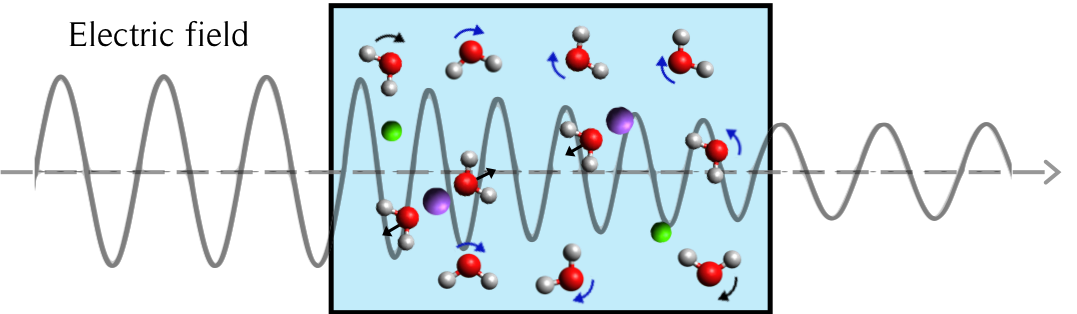
\includegraphics[width=0.85\figwidth]{chapters/Chapter1_Introduction/Graphs/DRS_Concept1.png} %The local modes are calculated on the XXX level, and reproduced with permission from ref. XXX. 
	\caption{Schematic representation of dielectric relaxation spectroscopy. If an external electric field is applied, water molecules will reorient towards the direction of the electric field. However, in the presence of ions, the degrees of rotational freedom of some water molecules are reduced or even locked in local structures referred to as solvation shells.}
	\label{DRSSchematic}
\end{figure}



Going one step further, we aim to determine hydration numbers by investigating the kinetic contribution to the depolarization experimental manner. In \textbf{Chapter~2}, we introduce the theoretical background and experimental methodology for the study of ion solvation using VNA-based DRS. In \textbf{Chapter~4}, we present a new method to extract hydration numbers based on the isotope dependence of the dielectric response. In this chapter, we aim to quantify the reduced cooperativity of water due to the local disruption  of the hydrogen-bond network. In \textbf{Chapter~5}, we apply this method to establish hydration numbers of a series of alkali-metal ions, and observe the ion-size dependence. Subsequently, in \textbf{Chapter~6}, we present similar analyses to estimate the number of water molecules affected by aqueous \ce{H+} and \ce{OH-} ions.



\subsection{Microscopic observation of solvating water molecules}



Femtosecond laser pulses have been used to perform ultrafast time-resolved vibrational spectroscopy (TRVS). This technique has been used to study molecular properties, e.g.\ molecular reorientation,\!\cite{Loparo2004,Rezus2005,Rezus2006,Thogersen2008,Shattuck2016} binding interactions,\!\cite{Eaves2005,Fecko2005,Baiz2015,Stevenson2015,Zhang2016} and energy equilibration.\!\cite{Woutersen1999,Piatkowski2009,Timmer2010} In this experimental approach, the way that light couples to the vibrational motion of molecules permits the exploration of structures down to the scale of a chemical bond ($\sim$1~\AA). An aspect of particular interest is that the vibrational resonances of molecules, as well as the associated vibrational relaxation rates, are sensitive to the structure and dynamics of the surrounding environment. This structure-dependent character allows us to assess the structural dynamics of solvating water molecules, as well as the properties of the hydrogen-bond network.



In particular, the vibrational properties of the hydroxyl groups of water molecules are affected by the hydrogen bonds that they donate, and consequently, by the strength of the hydrogen-bonding interactions in their vicinity.\!\cite{Lawrence2003,Auer2009,Bakker2010} A clear proof of this effect is observed in the OH-stretch resonance that shifts from 3657~cm$^{-1}$ in the gas phase (no hydrogen bonds) to lower frequencies around 3400~cm$^{-1}$ in the hydrogen-bonded liquid. This means that hydrogen bonds weaken the strength of the OH covalent bonds of water.



In electrolyte solutions, the vibrational dynamics of water molecules near ions further changes due to the strong local electric fields and the disruption of the hydrogen-bond network of water. In aqueous perchlorate (ClO$_4^{-}$) solutions, for example, there are two well-defined OH stretch bands: the first band associated with the bulk OH stretch vibration with a resonant frequency of 3400~cm$^{-1}$ and the second band at higher frequencies associated with OH oscillators that form weak hydrogen bonds with perchlorate ions.\!\cite{Timmer2010} One can thus selectively target and study the vibrational dynamics of solvating or bulk-like water molecules. As has been shown previously, TRVS experiments based on the OH stretch vibration are quite insensitive to the presence of cations.\!\cite{Omta2003,Omta2003a} This can be explained by the fact that no hydrogen bonds are donated to positive ions. This characteristic contrasts with DRS experiments.



\begin{figure}[t!]
	\centering
	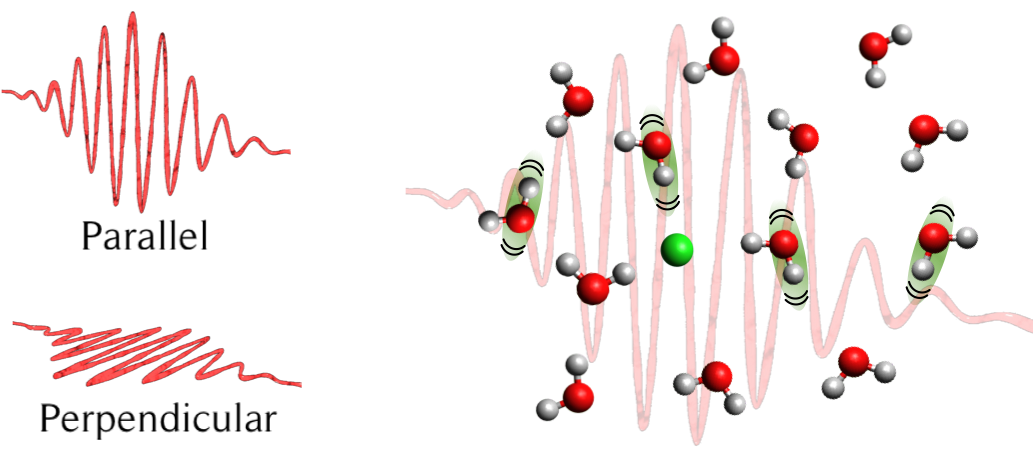
\includegraphics[width=0.85\figwidth]{chapters/Chapter1_Introduction/Graphs/TRVS_Concept1.png} %The local modes are calculated on the XXX level, and reproduced with permission from ref. XXX. 
	\caption{Schematic representation of time-resolved vibrational spectroscopy. An initial femtosecond pump pulse couples to local vibrational resonances of water molecules, which are afterwards tracked with a second femtosecond pulse called probe. In polarization-resolved TRVS, the sample is probed both in parallel and perpendicular configuration in order to observe molecular reorientation dynamics.}
	\label{TRVSSchematic}
\end{figure}


Polarization-resolved TRVS experiments provide direct information on the reorientation dynamics of the probed OH vibrations. Previous studies have shown a significant slowing down of the molecular dynamics upon the addition of ions. In fact, the reorientation dynamics of water in anionic solvation shells are strongly constrained to rotations within a cone around the axis defined by the directional hydrogen bond of the OH group to the anion.\!\cite{vanderPost2012,vanderPost2012a,vanderPost2013} In addition, the wiggling motion of the OH group bonded to the anion restricts the formation of hydrogen bonds between water molecules in the first solvation shell and the outer environment. Hence, the slow-down effect is limited to the first solvation shell, and the hydrogen-bond network is accordingly disrupted.\!\cite{Marcus2009} In contrast, aqueous sugar solutions have shown a slowing down effect that extends beyond the first solvation shell. This is explained by the fact that, instead of a disruptive effect, the hydroxyl groups of the sugar molecules form part of the hydrogen-bond network.\!\cite{Groot2014,Groot2015}


Protons (\ce{H+}) and hydroxide ions (\ce{OH-}) have the ability to form hydration complexes in which the excess charge is delocalized, and structural rearrangements lead to proton transfer between neighboring water molecules. This effect has been a fascinating subject of intense research in the last two decades. However, while a fairly large number of experimental efforts have been carried out on acid solutions,\!\cite{Woutersen2006,Moilanen2008,Peighambardoust2010,Liu2015,Fournier2018} only a few experimental studies in alkaline solutions have been reported.\!\cite{Roberts2009,Roberts2011,Mandal2014,Mandal2015,Biswas2017} As has been discussed before,\!\cite{Marx2010} this disparity can be explained from the classical view that hydroxide ions (\ce{OH-}, proton hole) mirror the effect of proton transfer via hydronium ions (\ce{H3O+}, proton excess). Nonetheless, recent theoretical studies have shown that \ce{OH-} and \ce{H3O+} ions have different structural properties, calling for the study of hydroxide ions as a subject of independent experimental research.\!\cite{Tuckerman2002,Chen2002,Sun2009,Bucher2010,Hassanali2011,Roberts2014,Chen2018a}


In \textbf{Chapter~3}, we introduce the theoretical background and experimental methodology for the study of intermolecular interactions in aqueous solutions using TRVS. \textbf{Chapters~7} and \textbf{8} focus on the study of structural properties in aqueous alkaline solutions using TRVS. In \textbf{Chapter~7}, we performed polarization-resolved measurements to explore whether hydroxide ions have an influence on the dynamics of water molecules beyond the first solvation shell. In \textbf{Chapter~8}, we explore whether the hydration complexes that hydroxide ions form can play a role in dissipating vibrational energy of surrounding molecules, an effect that has been observed in acidic solutions and has been attributed to the hydronium ion.\!\cite{Timmer2010} Finally, in \textbf{Chapter~9}, we study the solvation properties of aqueous phenolate ions using polarization-resolved TRVS and molecular dynamics simulations. 










% Add an empty page if needed to accomodate properly the chapter image
%%!TEX root = ../thesis.tex

\chapter*{}
%!TEX root = ../thesis.tex

\renewcommand\thefigure{\thechapter.\arabic{figure}}
\renewcommand{\thesection}{\thechapter.\arabic{section}}
\normalsize


\thispagestyle{empty}

\begin{tikzpicture}[remember picture,overlay]
\node at (current page.center) {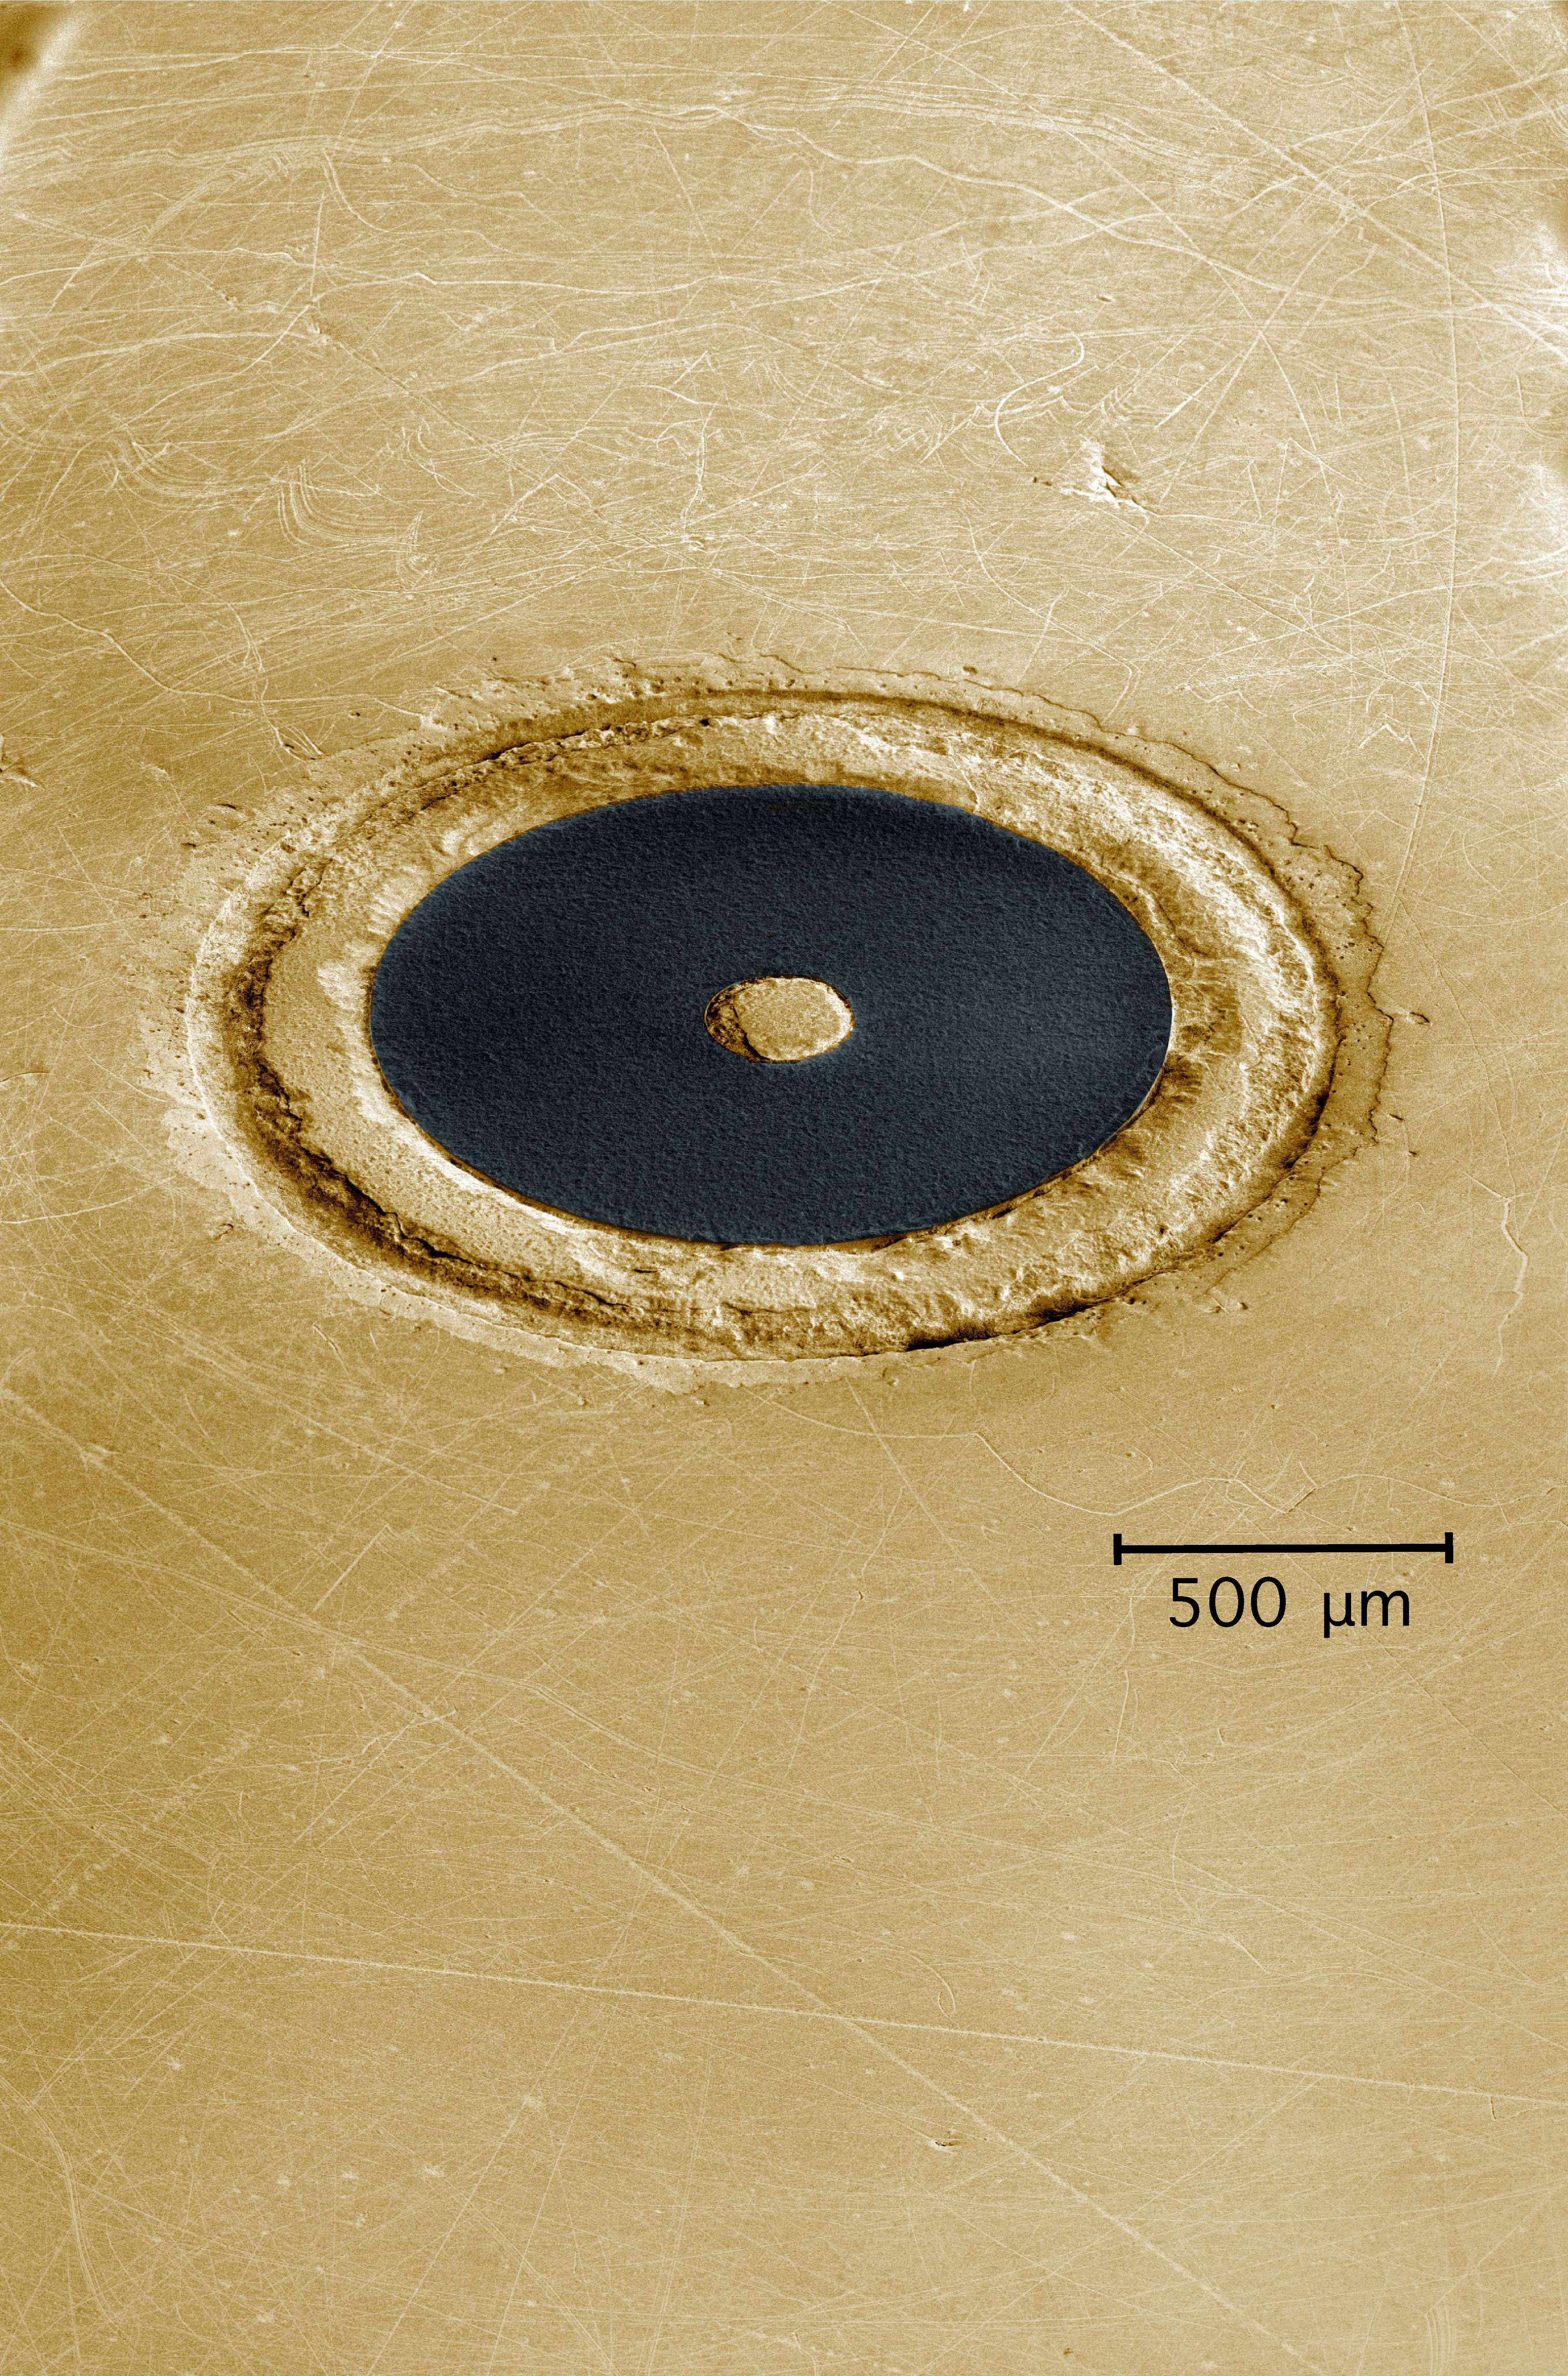
\includegraphics[width=\pdfpagewidth,height=\pdfpageheight]{fullpage_images/Head_SampleCell.pdf}};
\end{tikzpicture}

\clearpage



\begin{savequote}[75mm]
$\blacktriangleleft$ Top view of the coaxial-probe head used for dielectric relaxation measurements. The marks on the surface show the erosion caused throughout the experiments presented in Chapters 4--6.

\vspace{3pt}

SEM Photo, Lukas Helmbrecht. Edition, Roberto Cota
\end{savequote}




%\chapter{Dielectric relaxation spectroscopy\myfnt{{\it Sections~\ref{FormalismSection} and ~\ref{sec:VSFG-methods} of this chapter are based on:} S. J. Roeters, C. N. van Dijk, A. Torres-Knoop, E. H. G. Backus, R. K. Campen, M. Bonn, and S. Woutersen, \textit{The Journal of Physical Chemistry A} \textbf{117} (29), pp. 6311–6322 (2013).}}



\chapter[Methods I: Dielectric relaxation spectroscopy]{Methods I\\Dielectric relaxation spectroscopy}
\label{chap:methods1}
\label{MethodsChapter2}
\label{ChapterDRS}

\vspace{30pt}


The polarization properties of aqueous solutions, intimately linked to molecular structuring and solvation properties, are discussed in this chapter. First, we introduce the concept of dipole moment reorientation that results from the interaction with external electric fields. Then, we provide the microscopic molecular description underlying the observed macroscopic dielectric properties. As such, we can use dielectric relaxation spectroscopy to study molecular mobility and molecular cooperativity. If electrolyte solutions are our samples of interest, we can determine the extent to which ions affect the hydrogen bonding interactions of water. The discussion on the local ordering effect of water molecules in solvation shells is also one of the main goals of this chapter. Finally, the data analysis and modeling of the dielectric relaxation measurements are described.



\newpage



\section{Electromagnetic waves interacting with matter}\label{MolVibs}

A complete (classical) description of propagating electromagnetic fields can be performed by means of the Maxwell equations\!\cite{Jackson1999}
\begin{eqnarray}
\nabla \cdot \vec{D} &=& \rho_e, \label{GaussLaw} \\
\nabla \cdot \vec{B} &=& 0, \label{MagGaussLaw} \\
\nabla \times \vec{E} &=& - \frac{\partial \vec{B}}{\partial t}, \label{FaradayLaw} \\
\nabla \times \vec{H} &=& \vec{j} + \frac{\partial \vec{D}}{\partial t}, \label{AmpereLaw}
\end{eqnarray}
\noindent in which Eq.\ \ref{GaussLaw} shows that the electric displacement $\vec{D}$ is determined by the distribution of electric charges $\rho_e$. Gauss's law for magnetism, Eq.\ \ref{MagGaussLaw}, states that the net magnetic field $\vec{B}$ over a closed surface must be zero, meaning that magnetic monopoles cannot exist. The Maxwell-Faraday equation, Eq.\ \ref{FaradayLaw} describes the induction of electric fields as the result of time-varying magnetic fields. While Amp\`ere's law, Eq.\ \ref{AmpereLaw}, indicates the induced magnetic fields due to electrical currents and time-varying electric fields. 


For an homogeneous and isotropic material with intrinsic properties that are time-independent, one can derive the following three constitutive equations
\begin{eqnarray}
\vec{D} &=& \epsilon_0 \vec{E} + \vec{P} = \epsilon_0 \hat{\epsilon} \vec{E}, \label{DtoE} \\
\vec{B} &=& \mu_0 \vec{H} + \vec{M} = \mu_0 \hat{\mu} \vec{H}, \label{HtoB} \\
\vec{j} &=& \kappa \vec{E}, \label{ConduConstitutive}
\end{eqnarray}
\noindent where $\vec{P}$ and $\vec{M}$ are the polarization and magnetization density vectors, respectively. The material properties are described by the complex relative electric permittivity $\hat{\epsilon}$ and the complex relative magnetic permeability $\hat{\mu}$. These properties can also be expressed with the electric and magnetic susceptibilities of the material as $\hat{\epsilon} = 1 + \hat{\chi}_e$ and $\hat{\mu} = 1 + \hat{\chi}_m$. The quantities $\epsilon_0$ and $\mu_0$ describe the permittivity and permeability of free space. The quantity $\kappa$ is the specific conductivity of the material. It is important to notice that Eqs.\ \ref{GaussLaw}-\ref{ConduConstitutive} constitute a set of linear equations to compute all kind of electromagnetic interactions.



From Eq.\ \ref{DtoE}, one can observe that the electric displacement results from the polarization response of the material due to electric forces. This polarization response can involve  a displacement of the electron cloud of atoms or molecules with respect of the unperturbed state. It can also involve the reorientation of a dipolar molecular towards the direction of the electric field $\vec{E}$. In the case of static electric fields, the complex permittivity reduces to the so-called static permittivity $\epsilon_\text{s}$, which is also commonly referred to as dielectric constant. The latter quantity defines the total static polarization. 



Due to microscopic interactions and inertial effects, the reaction of the medium to an applied external electric field is not instantaneous. Instead, the system requires a time interval to reorient following the direction of the external field, meaning that the polarization effect is delayed with respect to the electric field $\vec{E}$. If we consider a monochromatic oscillating electric field $\vec{E}(t) = \vec{E}_0 cos (\omega t)$ with amplitude $\vec{E}_0$, a phase shift between $\vec{D}$ and $\vec{E}$ will emerge that depends on the frequency $\omega$:
\begin{eqnarray}
\vec{D} (t) = \vec{D}_0 \cos [\omega t -\delta (\omega)],
\label{DisplacementDelay1}
\end{eqnarray}
\noindent with $\delta(\omega)$ the frequency-dependent phase delay, which is also referred to as loss angle. Notice that $\vec{D}_0 = \epsilon_0 \hat{\epsilon}(\omega) \vec{E}_0$ according to Eq.\ \ref{DtoE}.



By introducing the following reciprocal representation in the complex plane
\begin{eqnarray}
\vec{D}_0 [\cos \delta - i \sin \delta ] = \epsilon_0 \vec{E}_0 [\epsilon' - i \epsilon''],
\end{eqnarray}
\noindent the electric displacement given in Eq.\ \ref{DisplacementDelay1} can be expressed with the following formula
\begin{eqnarray}
\vec{D} (t) = \epsilon'(\omega) \epsilon_0 \vec{E}_0 \cos(\omega t) +  \epsilon'' (\omega) \epsilon_0 \vec{E}_0 \sin(\omega t).
\label{DisplacementDelay2}
\end{eqnarray}



The preceding equation shows that the electric displacement arises from two effects with different nature: (i) the in-phase dielectric dispersion is proportional to the real part of the relative permittivity, while (ii) the out-of-phase dielectric dissipation (dielectric loss) is proportional to the imaginary part of the relative permittivity. It is clear from Eq.\ \ref{DisplacementDelay2} that the mathematical formulation can be promoted to complex notation, i.e.\ $ \hat{\vec{D}} = \epsilon_0 \hat{\epsilon} \hat{\vec{E}}$. Notice that a similar delayed response can occur between the magnetic flux $\vec{B}$ and the magnetic field strength $\vec{H}$, and therefore Eq.\ \ref{HtoB} can be analogously written as Eq.\ \ref{DisplacementDelay2}.



One can describe the evolution of the electromagnetic fields as plane waves with the following functional forms
\begin{eqnarray}
\hat{\vec{E}} (\vec{r},t) &=& \hat{\vec{E}} (\vec{r}) \exp (i \omega t),\\
\hat{\vec{H}} (\vec{r},t) &=& \hat{\vec{H}} (\vec{r}) \exp (i \omega t),
\label{harmonicoscillators}
\end{eqnarray}
\noindent which in combination of Eqs.\ \ref{GaussLaw}--\ref{ConduConstitutive} (with a net electric charge of zero, i.e\ $\nabla \cdot \vec{D} = 0$) lead to the following wave equations
\begin{eqnarray}
\nabla^2 \hat{\vec{E}} (\vec{r}) + \hat{k}^2 \hat{\vec{E}} (\vec{r}) &=& 0 ,
\label{helmholtzeq1}
\\ \nabla^2 \hat{\vec{H}} (\vec{r}) + \hat{k}^2 \hat{\vec{H}} (\vec{r}) &=& 0,
\label{helmholtzeq2}
\end{eqnarray}
\noindent that describe the propagation of electromagnetic waves through a material. A solution to Eq.\ \ref{helmholtzeq1} is given by $\vec{E} (\vec{r}) = E_0 \exp(i \vec{k} \cdot \vec{r})$, where $\hat{k}$ is the wave vector expressed by 
\begin{eqnarray}
\hat{k}^2 = k_0^2 \left[ \hat{\mu} (\omega) \hat{\epsilon} (\omega) + \frac{\hat{\mu} (\omega)  \hat{\kappa} (\omega)} {i \omega \epsilon_0}   \right].
\label{wavenumberP}
\end{eqnarray}
\noindent with $k_0 (= \omega \sqrt{\mu_0 \epsilon_0} = \omega/c  )$ the propagation constant in vacuum. The preceding equation describes the response of a medium to electromagnetic fields, and shows the extent to which the propagation of the field deviates from that observed in free space.


For electrolyte solutions, which are the focus of interest in this work, the wave vector can be written as
\begin{eqnarray}
\hat{k}^2 = k_0^2 \left[ \hat{\epsilon} (\omega) + \frac{  \sigma} {i \omega \epsilon_0}   \right],
\label{wavenumberP2}
\end{eqnarray}
\noindent where $\hat{\kappa} (\omega)$ reduces to the DC ionic conductivity $\sigma$, since its frequency dependence is irrelevant in the frequency range of our interest ($\sim$18 GHz the characteristic dielectric relaxation mode of water).\!\cite{Ghowsi1989,Anderson1994a,Ellison1996,Buchner1999b}

In electrolyte solutions, the energy loss (imaginary part) arises from the non-instantaneous rearrangement of charges in the dielectric medium, as well as from the work exerted by rotating dipoles. The real part of the dielectric dispersion is related to the temporarily stored energy, and determined by the degree of orientation of the dipoles along the direction of the electric field.


% $\hat{\kappa}$ reduces to the DC ionic conductivity $\sigma$, since the frequency-dependent character of $\hat{\kappa}$ is irrelevant in the frequency range of our interest ($\sim$~20 GHz the characteristic dielectric relaxation mode of water)~\cite{Ghowsi1989,Anderson1994a,Buchner1999b}. 







\section{Polarization}



The polarization of a medium can be defined as the net macroscopic dipole per volume of a medium in the presence of an electric field. From Eq.\ \ref{DtoE}, one can write
\begin{eqnarray}
\hat{\vec{P}} = (\hat{\epsilon} - 1) \epsilon_0  \hat{\vec{E}},
\label{polarizationvector}
\end{eqnarray}
\noindent in which the polarization is described as the dielectric response of the medium to $\hat{\vec{E}}$. The underlying microscopic definition can be understood as the sum of two contributions
\begin{eqnarray}
\hat{\vec{P}} = \hat{\vec{P}}_\mu + \hat{\vec{P}}_\alpha
\label{polarizationvectorSeparation}
\end{eqnarray}
where $\hat{\vec{P}}_\mu$ refers to the orientational response of molecular dipoles, while $\hat{\vec{P}}_\alpha$ is attributed to the polarization resulting from the intramolecular polarizability. 





These two contribution are generally well separated. The orientational relaxation of dipoles along the applied electric field typically takes place in the order of picoseconds or slower, such as the dielectric response of water with a time constant of $\sim$8 ps at room temperature. While the molecular polarizability takes place at the femtosecond timescale. Thus, $\hat{\vec{P}}_\mu$ and $\hat{\vec{P}}_\alpha$ are considered independent with each other, leading to
\begin{eqnarray}
\hat{\vec{P}}_\mu = \epsilon_0 (\hat{\epsilon} - \epsilon_\infty) \hat{\vec{E}} \label{separationPolarization1}, \qquad \text{and} \qquad \hat{\vec{P}}_\alpha = \epsilon_0 (\epsilon_\infty - 1) \hat{\vec{E}},
\label{separationPolarization2}
\end{eqnarray}
\noindent with $\epsilon_\infty$ the permittivity in the intermediate frequency region at which dipoles are insensitive to the fast oscillating field, but the molecular polarizability has attained its maximum amplitude. Experiments focused on the dipolar orientation effect in aqueous solutions have shown that $\epsilon_\infty$ is constant in the GHz frequency region.\!\cite{Lileev2007} In the limit of a static electric field ($\omega \to 0$), the orientational polarization reduces to $\vec{P}_{\mu,0} = \epsilon_0 ( \epsilon_{\text{s}} - \epsilon_\infty) \vec{E}_0 $. The static permittivity $\epsilon_\text{s}$ is attained when all types of polarizations reach equilibrium with a switched-on DC electric field. The microscopic description is discussed in the following section.



\section{Microscopic description of static permittivity}



The macroscopic static permittivity can be connected to the microscopic notion of the collection of molecular dipoles aligned along the direction of the external field. 



Under the action of an electric field, dipoles tend to reorient towards the direction of the electric field in order to minimize their internal energy, defined as
\begin{eqnarray}
U (\theta) = - \vec{\mu} \cdot \vec{E} = - \mu E \cos{\theta},
\label{PotentialPolarization}
\end{eqnarray} 
where $\theta$ represents the angle between the dipole moment vector $\vec{\mu}$ and the electric field vector $\vec{E}$. Thus, it is clear to see that the minimum energy is attained at $\theta=0$, which mean a perfect alignment to the electric field. Such a situation is physically unaccessible since it means a system in perfect order with no entropy--this could theoretically occur at extremely low temperatures at which, ironically, the molecules would not have enough energy to rotate and align with the electric field. At non-zero temperatures the molecules will diffuse and rotate constantly because of the thermal energy of the system. 



Under the action of an external electric field, the orientation of the dipoles is slightly shifted from the random distribution, leading to an effective (averaged) dipole moment $\langle \vec{\mu} \rangle$. If we assume that the medium is formed by only one type of dipoles, the polarization can be written as
\begin{eqnarray}
\vec{P} = \rho \langle \vec{\mu} \rangle,
\label{GeneratlPolarization}
\end{eqnarray} 
which is proportional to the density $\rho$ of dipolar molecules.



In this view, the system is formed by dipoles with a statistical distribution between $\theta_\text{min} = 0 $ and $\theta_\text{max} = \pi$. The Boltzmann distribution equation can be used to determine the fraction of dipoles with a certain energy $U$:
\begin{eqnarray}
N (U) = A \exp \left( - \frac{U(\theta)} {k_\text{B} T} \right) 
\label{BoltzmannDistri}
\end{eqnarray} 
with $T$ and $k_\text{B}$ the temperature of the system and the Boltzmann constant, respectively. Given the preceding equation, the averaged dipole moment can be obtained summing up the contribution of all possible states, as follows
\begin{eqnarray}
\langle \vec{\mu} \rangle = \frac{ \int_0^\pi N[U(\theta)] \cdot \mu \cos \theta \cdot d\Omega     } {   \int_0^\pi N[U(\theta)] \cdot d\Omega   }
\label{AveragedMoment1}
\end{eqnarray} 
\noindent where $d\Omega$ ($= 2\pi \sin\theta d\theta$) is the solid angle increment on a unit sphere when $\theta$ changes to $\theta + d \theta$. Notice that $\Omega$ account for the three-dimensional system, in which the polarization is invariant to rotations over the azimuthal angle around the electric field vector. The solution to Eq.\ \ref{AveragedMoment1} yields $\langle \vec{\mu} \rangle = \mu \text{L}(\xi)$, with $\text{L}$ the Langevin equation, and $\xi = \mu E/ k_\text{B} T$. In the limit of $\xi \ll 1$ (which is valid even for very strong electric fields and strong dipoles), $\text{L} (\xi) \simeq \xi/3 $, we reach to the Langevin-Debye equation for the induced polarization is obtained\!\cite{DebyeBook1929,Evans1982}
\begin{eqnarray}
\vec{P} = \frac{\rho \mu^2}{3 k_\text{B} T} \vec{E} = \epsilon_0 (\epsilon_\text{s} - \epsilon_\infty) \vec{E},
\label{LangeDebyePolarization}
\end{eqnarray} 
and thus:
\begin{eqnarray}
\epsilon_\text{s} - \epsilon_\infty = \frac{\rho \mu^2}{3 \epsilon_0 k_\text{B} T}.
\label{FirstDielectricConstant}
\end{eqnarray} 



\subsection{The Lorentz cavity field and Debye's theory of dielectrics}



The above description assumes that each molecule is solely affected by the action of the external field, and the total polarization is the result of the collection of individual contributions. However, a dipole immerse in the system will be also affected by the macroscopic polarization of the system $\vec{P}$. The force that a given polar molecules experiences arises from the sum of the external field and the collective polarization of the system, such that 
\begin{eqnarray}
\vec{E}_\text{loc} = \vec{E} + \frac{\vec{P}}{3 \epsilon_0} \qquad \Longrightarrow \qquad \vec{E}_\text{loc} = \frac{\epsilon_\text{s} + 2}{3} \vec{E},
\label{LorentzField}
\end{eqnarray} 
which is known as the Lorentz cavity field.\!\cite{Lorentz1916} In this approach, one assumes that each dipole is inside a small spherical cavity with a charge distribution at the surface as the result of the macroscopic polarization. As can be seen in Eqs.\ \ref{GeneratlPolarization} and \ref{LorentzField}, the Lorentz field acts parallel to the applied field $\vec{E}$ and effectively enhances the response of the dipoles. 



Debye was the first one to use this notion to model the temperature-dependent dielectric constant, which Eq.\ \ref{FirstDielectricConstant} failed to predict. With this approach Debye derived
\begin{eqnarray}
\frac{\epsilon_\text{s} - 1}{\epsilon_\text{s} + 2} = \frac{\rho \mu^2}{9 \epsilon_0 k_\text{B} T} + \frac{\rho \alpha}{3 \epsilon_0},
\label{DebyeDielectricConstant}
\end{eqnarray} 
or if we consider the Clausius-Mossotti relation for molecular polarizability $\alpha$,\!\cite{choy1999effective} the dielectric constant can be written as
\begin{eqnarray}
\frac{\epsilon_\text{s} - 1}{\epsilon_\text{s} + 2} - \frac{\epsilon_\infty - 1}{\epsilon_\infty + 2} = \frac{\rho \mu^2}{9 \epsilon_0 k_\text{B} T},
\label{DebyeDielectricConstant2}
\end{eqnarray} 
which is limited to estimate the dielectric response of gases and dilute solutions of polar molecules in non-polar solvents due to assumptions in defining Eq.\ \ref{LorentzField}. %In this framework the central dipole is affected by the resultant field from neighbouring polar molecules, while the field generated by the central dipole is assumed negligible. This means that the medium is not influenced by the presence of the cavity, which is not entirely valid.  



Furthermore, if the term for polarizability is neglected, one can derive a critical behavior for the dielectric constant with the following functional form
\begin{eqnarray}
\epsilon_\text{s} = \frac{T + 2 T_c}{T - T_c}, \qquad \text{with} \qquad T_c = \frac{\rho \mu^2}{9 \epsilon_0 k_\text{B}},
\label{DebyeCritical}
\end{eqnarray} 
that defines a critical temperature $T_c$ at which the dielectric response would diverge. Near $T_c$, the polarization becomes so large, meaning extremely large local electric fields, that the dipoles would align to one another even in case of $E \sim 0$ (analogous to a permanent magnet!). This problem and limitations were spotted and criticized by Onsager.~\footnote{Onsager submitted a paper with a criticism of Debye's theory to \textit{Physikalische Zeitschrift} at which Debye was the editor by the time. It got rejected.\!\cite{ChristopherLonguet-Higgins1995}} Onsager derived a more strict model by noting that for dipolar molecules the local electric field differs from the average electric field that results from the polarization of all molecules in the medium.



\subsection{Onsager equation of dielectrics}



Onsager described the dielectric response as the contribution of polar molecules contained in spherical cavities with radius $a$, in which the sum of all the spheres equals to the volume of the material.\!\cite{Onsager1936,BOTTCHER1973} He started by computing the electric field in a spherical cavity resulting from the applied field in the dielectric medium surrounding the cavity, and the electric field resulting from the back reaction of the medium on the dipole moment of the molecule in the cavity.


%He started by computing the field produced by the dipole inside and outside the sphere, in which boundary conditions should be satisfied. Hence, Onsager's theory considers that the outer medium is affected by the presence of the polar cavity.



Within this model, the internal field acting on a given dipole consist of two contributions: (i) the cavity field generated which is parallel to the external field, and (ii) the reaction field resulting from the back reaction of the surrounding medium to the dipole in the cavity. Under the influence of these two fields, the confined dipole will be polarized so that its instantaneous dipole moment differs from its permanent dipole moment $\vec{\mu}$.\!\cite{Wilson1939}



Onsager was able to establish the following relation between dielectric constant, polarizability and vacuum dipole moment:
\begin{eqnarray}
\frac{ (\epsilon_\text{s} - \epsilon_\infty)   (2 \epsilon_\text{s} + \epsilon_\infty)    }{\epsilon_\text{s} (\epsilon_\infty +2)^2  } = \frac{\rho \mu^2}{9 \epsilon_0 k_\text{B} T},
\label{OnsagerDielectricConstant2}
\end{eqnarray}
which does not contain singularities, in contrast to Debye's description. This equation offers a better description for the dielectric constant of polar liquids.\!\cite{Wilson1939,Buchner1999b,Buchner1999}



\subsection{Kirkwood-Fr\"ohlich equation of dielectrics}\label{KirkFrohSection}


In the approaches of Debye and Onsager, the dielectric response has been established based on a continuum description of the dielectric medium, but the effect of intermolecular interactions has been neglected. Aqueous systems, which are of our interest, tend to behave in a cooperative manner. Kirkwood and later Fr\"ohlich performed a rigorous statistical study of the intermolecular interactions to extend the Onsager equation of dielectrics.\!\cite{Kirkwood1939a,BOTTCHER1973,Frohlich1986} They derived the following expression
\begin{eqnarray}
\frac{ (\epsilon_\text{s} - \epsilon_\infty)   (2 \epsilon_\text{s} + \epsilon_\infty)    }{\epsilon_\text{s} (\epsilon_\infty +2)^2  } = \frac{\rho \mu^2 g_\text{K}}{9 \epsilon_0 k_\text{B} T},
\label{KirkFroConstant}
\end{eqnarray}
\noindent where $g_\text{K}= 1 + z \langle \cos \gamma \rangle$ is the Kirkwood correlation factor which is a measure of the microscopic ordering of the medium. In the latter expression for $g_\text{K}$, $z$ is the solvation number and $\langle \cos \gamma \rangle$ is the average orientation between two neighbouring dipoles. Notice that in the limit $g_\text{K} = 1$, which corresponds to a completely uncorrelated orientation of the dipoles, Eq.\ \ref{KirkFroConstant} reproduces the expression of Onsager. In case that dipoles cooperate in a parallel manner $g_\text{K} > 1$, while $g_\text{K} < 1$ means that neighbouring dipoles have an antiparallel character. For liquid water a Kirkwood correlation factor of $2.7$ has been observed.\!\cite{Buchner1999b} Then, it is clear that the structure of water increases the dielectric response with respect to an uncorrelated orientation.






\section{Dielectric relaxation}\label{DRTheory}


The previous section has discussed the microscopic picture of polarization, under the assumption of static electric fields. The following question concerns to the dynamic permittivity in oscillating electric fields.

Let us start with a dielectric medium in its static $\vec{P}_{\mu,0}$ state, if the electric field is switched off, the polarization vector will decay due to thermal motions. The simplest assumption is to assume that the polarization decay follows a first-order differential equation as
\begin{eqnarray}
\frac{d \hat{\vec{P}}_\mu (t)}{d t } = - \frac{\hat{\vec{P}}_\mu (t)}{\tau_\text{D}}.
\label{FirstOrderDecay}
\end{eqnarray}




To determine the dielectric spectrum, we use the Fourier transformation to express the polarization in the frequency domain, therefore Eq.\ \ref{FirstOrderDecay} yields 
\begin{eqnarray}
\hat{\vec{P}}_\mu (\omega) =  \frac{\vec{P}_{\mu,0}}{1 + i \omega \tau_\text{D}},
\label{FouriertranformP}
\end{eqnarray}
\noindent which combined with Eq.\ \ref{separationPolarization1} leads to 
\begin{eqnarray}
\hat{\epsilon} (\omega) =  \epsilon_\infty + \frac{ \epsilon_\text{s} - \epsilon_\infty }{1 + i \omega \tau_\text{D}}.
\label{DebyeRelaxation}
\end{eqnarray}







The preceding equation is the well-know Debye dielectric relaxation mode,\!\cite{DebyeBook1929,Debye1934} which assumes that all the microscopic dipoles respond with a single relaxation time $\tau_\text{D}$. In Eq.\ \ref{DebyeRelaxation}, $A_\text{D} = \epsilon_\text{s} - \epsilon_\infty$ determines the strength of the Debye relaxation mode. As shown in Figure \ref{RelaxationModes}, the dielectric loss is maximum when the frequency of the external electric field matches the Debye relaxation time. 





The Debye model considers a single-exponential relaxation which provides a good description of the relaxation mechanism of pure solvents, such as water.\!\cite{Buchner1999b,Buchner2008} However, systems in which the neat structure is perturbed, the relaxation process can comprise a rather broader distribution of relaxation times. Nonetheless, the analytical approach is difficult, a series of empirical models have been offered to account for such deviations. The most general approach to account for this distribution is the Havriliak-Negami equation\!\cite{Havriliak1966}
\begin{eqnarray}
\hat{\epsilon} (\omega) =  \epsilon_\infty + \frac{ \epsilon_\text{s} - \epsilon_\infty }{[1 + (i \omega \tau_\text{D})^{1-\alpha} ]^\beta},
\label{RelaxationHavriNega}
\end{eqnarray}
\noindent in which the empirical parameters $\alpha$ and $\beta$ account for symmetrical and asymmetrical spectral broadening, respectively. When $\beta = 1$ the equation reduces to the so-called Cole-Cole relaxation mode,\!\cite{Cole1941a,Cole1955} which has been shown to be a good approach to model the relaxation process in electrolyte solutions.\!\cite{Kaatze1993,Nortemann1997,Buchner1999,Ottosson2014c,Cota2018} If $\alpha = 0$ and $\beta = 1$, Eq.\ \ref{RelaxationHavriNega} recovers the mono-exponential Debye relaxation process. The upper panel in Figure \ref{RelaxationModes} shows the contrast between the Cole-Cole mode and the Debye mode. 


\newpage

\begin{figure}[h!]
	\centering
	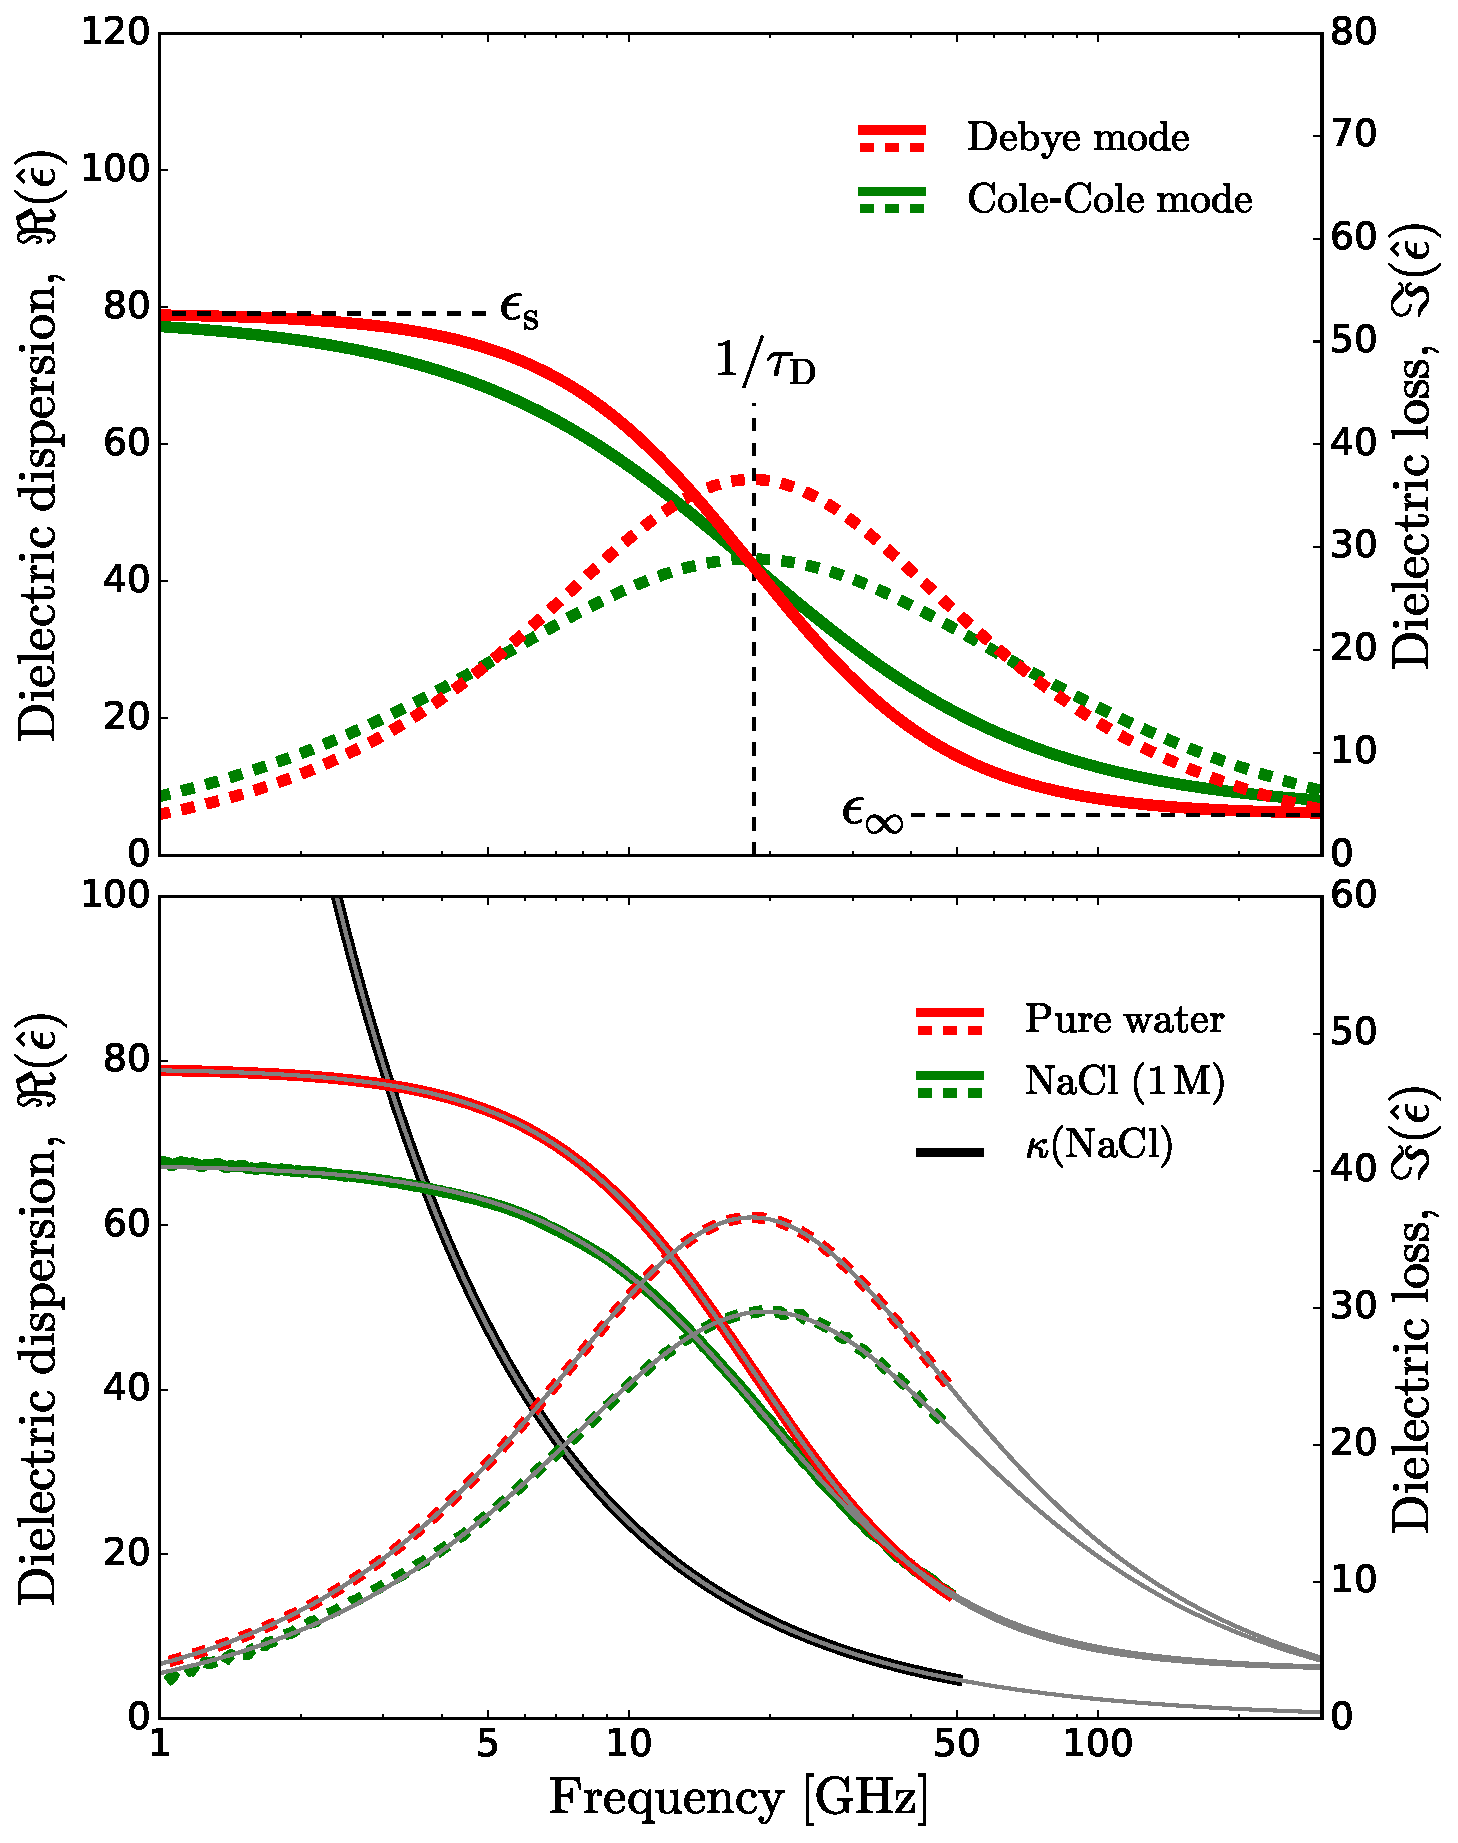
\includegraphics[width=0.85\figwidth]{chapters/Chapter2_Methods/Graphics/DebyeCole_Modes.pdf}
	\caption{The \textbf{upper panel} shows the band shapes of the Debye relaxation mode and the Cole-Cole relaxation mode. In both cases $A_\text{D} = 80$, $\epsilon_\infty = 6$ and $\tau_\text{D} = 8.7$ ps which corresponds to the dielectric properties of pure water at 23$^o$C,\!\cite{Buchner1999b,Ellison1996} while the Cole-Cole deviates from the Debye band by $\alpha = 0.15$. Solid lines represent the dielectric dispersion, and dashed lines the dielectric loss. The \textbf{lower panel} displays dielectric spectra for pure water and a 1 M \ce{NaCl}:\ce{H2O} solution. The corresponding dielectric loss of the alkaline solution has been corrected for the ionic conductivity, which is shown in black. From the dielectric constant at low frequencies, it is clear that the amplitude of the polarization is reduced in the presence of ions, an effect called depolarization. The solid grey curves result from fits using the Debye and the Cole-Cole modes for pure water and the alkaline solution, respectively.}
	\label{RelaxationModes}
\end{figure}


\newpage




For a conducting material, such as electrolyte solutions, the macroscopic dielectric response is modeled with the following generalized permittivity
\begin{eqnarray}
\hat{\eta} (\omega) = \epsilon_\infty + \frac{\epsilon_\text{s} - \epsilon_\infty }{1 + (i \omega \tau_\text{D})^{1-\alpha}} - \frac{i \sigma}{\epsilon_0 \omega},
\label{ColeConRelaxation}
\end{eqnarray}
\noindent which has shown to be sufficient to model the dielectric spectra reported in this thesis. The lower panel in Figure \ref{RelaxationModes} displays dielectric spectra for pure water and a 1 M \ce{NaCl}:\ce{H2O} solution both at 23$^o$C. The Debye mode is well suited to fit the spectra of pure water, while the electrolyte solution is fitted using a Cole-Cole mode showing a broadening of $\alpha = 0.02$. Therefore, the presence of ions induce a relaxation distribution that differs from the single exponential decays.





Moreover, in many systems the dielectric response rises from the contribution of multiple dipolar species, as in aqueous taurine solutions where taurine molecules also align with the electric field,\!\cite{Smit2019} or the discrete dynamics of water in tetramethylurea solutions.\!\cite{Tielrooij2010a} In these cases the dielectric spectrum can be model as the sum of $n$ independent relaxation processes.




\section{Depolarization}\label{SectionDepola}


In electrolyte solutions, ion generate strong local electric fields, orienting the dipoles of neighbouring water molecules. These interactions induce local ordering and reduce (locally) the degrees of orientational freedom of the water, an effect generally called depolarization. This effect reduces the absolute magnitude of the dielectric constant (static permittivity), as is shown in the lower panel of Figure \ref{RelaxationModes}. This depolarization can be described by the sum of three contributions: 

\begin{figure}[t!]
	\centering
	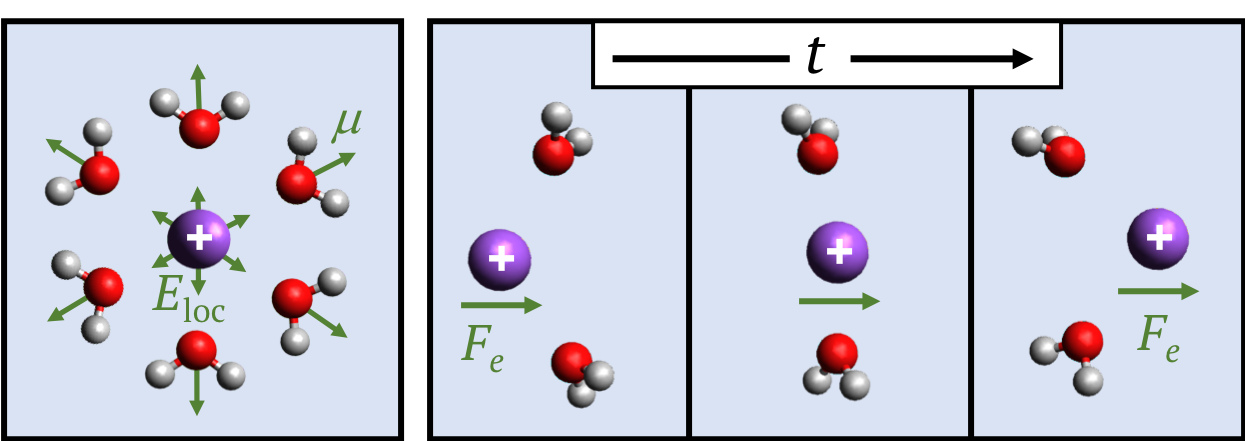
\includegraphics[width=1\figwidth]{chapters/Chapter2_Methods/Graphics/IonicDepolarization.png}
	\caption{\textbf{Left panel:} Static depolarization induces strong binding of water molecules leading to hydration shells. \textbf{Right panel:} Kinetic depolarization rises due to the rotational response of water molecules to the translational motion of ions. Here, $\mu$ is the permanent dipole moment of a water molecule, $E_\text{loc}$ the ionic electric field, and $F_e$ is the driving force that an ion experiences in the presence of a external electric field. The figures are exaggerated representations for conceptual purposes.}
	\label{IonicDepolarization}
\end{figure}

\begin{itemize}
	\setlength{\itemsep}{0pt}%
%	\setlength{\parskip}{2pt}}%
	\item{Dilution of the solvent: having a finite size, the excluded volume of ions leads to reduction in the density of water molecules with respect to the pure solvent.\!\cite{Onsager1936,BOTTCHER1973,Liszi1988} The amplitude of this effect is given by
	\begin{eqnarray}
	A_{\text{D},n} (c) = \frac{c_\text{w} (c)}{c_\text{w,0}} A_\text{D,0} 
	\label{dilutioneffect}
	\end{eqnarray}
	where $c_\text{w,0}$ and $A_\text{D,0}$ are the molecular concentration and the amplitude of the Debye relaxation mode of pure water, and $c$ is the ion concentration. The amplitude of the Debye relaxation mode $A_{\text{D},n} (c)$ scales linearly with the density of water molecules, which is consistent with the Onsager model of Eq.~\ref{KirkFroConstant} since the dielectric response of water is dominated by the reorientation of the dipoles, leading to the approximation that $2 \epsilon_\text{s} + \epsilon_\infty \approx 2 \epsilon_\text{s}$. As a result, the dielectric response $\epsilon_\text{s} - \epsilon_\infty$ of Eq.~\ref{KirkFroConstant} is directly proportional to the density. Eq.~\ref{dilutioneffect} assumes that the dilution does not lead to a change of the Kirkwood correlation factor $g_\text{K}$ of the remaining water in the solution.}
	





	\item{Static depolarization: the strong ionic field induces local ordering in solvation shells, locking the orientational motion of solvating water molecules\!\cite{Impey1983,Barthel1992} (see Figure \ref{IonicDepolarization}). Static depolarization $\Delta A_{\text{D,sta}}$ is linked to ionic hydration numbers\!\cite{Buchner2008} as follows
	\begin{eqnarray}
	Z_\text{hyd} = \frac{c_{w,0}}{A_{\text{D},0}} \frac{\Delta A_{\text{D,sta}} (c) }{c}.
	\end{eqnarray}
	One should take the nature of hydration around cations and anions into account. Static depolarization is generally attributed to cations because they constrain the degrees of orientational freedom of water much more than anions (see Figure \ref{BindingIons}). As such, the relative contribution of the anions to the static depolarization is negligible.\!\cite{Barthel1992,Buchner1999,Impey1983,Guardia1990,Ohtaki1993,Smith1994,Wachter2007}}

	\item{Kinetic depolarization: the long-range orientational response of water molecules to moving ions. An ion moving along the direction of the external electric field causes an opposite orientation of the solvent dipoles as compared to that caused by the external electric field.\!\cite{Hubbard1977a,Hubbard1977,Hubbard1978c,Hubbard1979a,VanderZwan1982,VanderZwan1983a}}
\end{itemize}



\begin{figure}[t!]
	\centering
	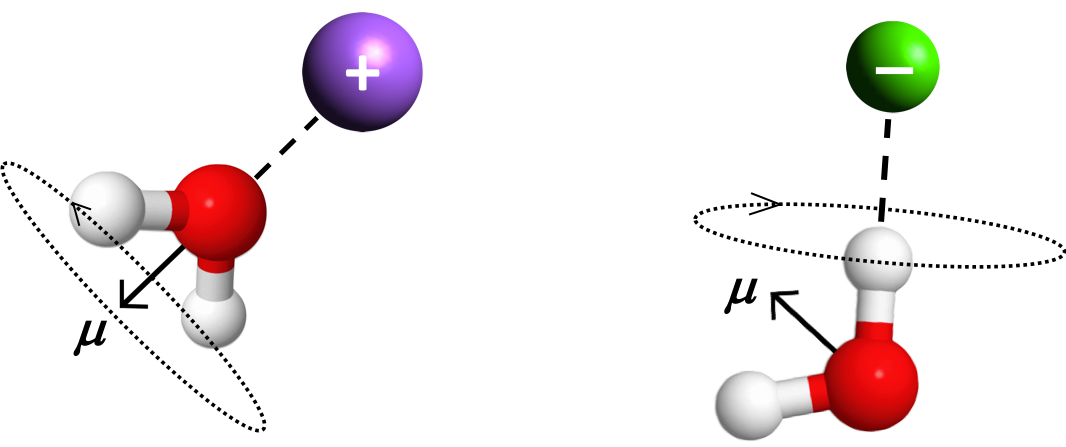
\includegraphics[width=0.7\figwidth]{chapters/Chapter2_Methods/Graphics/BindingIons.png}
	\caption{Static binding in the ionic vicinity. Water molecules hydrating cations are bounded along their dipole symmetrical axis, leading to a negligible orientation motion of the dipole. Hence, water molecules hydrating cations are assumed frozen with respect to the macroscopic dielectric response. On the other hand, water molecules in the anionic vicinity bond along the direction of one of their hydroxyl groups, providing still degrees of rotational motion to the permanent dipole moments.}
	\label{BindingIons}
\end{figure}



The amplitude of depolarization has been widely used to investigate local structuring in solvation shells. However, the static and kinetic contributions are difficult to separate experimentally.\!\cite{Cota2018} Over the last five decades the common approach was to compute the amplitude of kinetic depolarization from theoretical predictions. Hence, the difference between the experimentally obtained depolarization (corrected for dilution) and the value obtained theoretically was assigned to static depolarization, which was used to estimate hydration numbers.\!\cite{Buchner1999,Buchner1999c,Chen2003,Tielrooij2009,Buchner2008,Ensing2013,Sega2014,Ottosson2014c}




The Hubbard-Onsager continuum model for dielectric deficiency\!\cite{Hubbard1977a,Hubbard1977,Hubbard1978c} has been widely used to estimate the magnitude of kinetic depolarization.\!\cite{Hall1981,Nortemann1997,Kaatze1997,Buchner1999,Buchner1999c,Chen2003,Tielrooij2009,Buchner2008,Ensing2013,Sega2014,Ottosson2014c} This model assumes that the ions are immersed in a continuum environment with uniform dielectric behavior as that in pure water. Within this model, it is also assumed that the viscous friction is much larger than the dielectric drag that the orientating dipoles could cause on the ions. Based on these assumptions, the following expression for kinetic depolarization is obtained:
\begin{eqnarray}
\Delta A_{\text{D,kin}} (c) = p \sigma (c)  \left(  \frac{\tau_\text{D}}{\epsilon_0} \cdot    \frac{\epsilon_\text{s} - \epsilon_\infty}{\epsilon_\text{s}}     \right),
\label{HubOnsaKin}
\end{eqnarray}
\noindent where the values between the parenthesis are the dielectric properties of the pure solvent. This equation implies that twater molecules would react to the field of moving ions via a dielectric relaxation mechanism that is the same as the macroscopic dielectric relaxation. 



Hence, changes in the amplitude of kinetic depolarization depend only on the concentration-dependent ionic conductivity $\sigma (c)$, and the factor $p$ that characterizes the frictional forces at the ionic surface. Hubbard and Onsager also derived the values for the $p$-factor, with limiting cases of $p=1$ for a infinite frictional force at the ionic surface (stick) and $p=2/3$ for a negligible friction on the ionic surface (slip). 



It is clear that this model does not account for the ion specificity. In fact, the model implicitly assumes that water preserves the same local structure and ordering regardless the presence of ions, meaning that the cooperative molecular behavior is unperturbed in solvation shells (see Section \ref{KirkFrohSection}).  However, this assumption is contradictory to the notion of ions as structure breakers and structure makers, which have been determined from experiments and simulations.\!\cite{Marcus2009,Shattuck2016} This discrepancy is addressed in Chapter \ref{ChapterPRL}.



\section{Experiment realization}\label{ExperimentalDRS}


Dielectric relaxation spectroscopy enables us to measure the induced complex polarization of a sample in the frequency domain, which in consequence provides the characteristic complex permittivity $\hat{\epsilon} (\omega)$. Vector network analyzers (VNA) are a novel tool to study dielectric properties due to their capacity to measure simultaneously the phase and amplitude of electromagnetic waves in a wide range of frequencies. The used experimental setup is based on a vector network analyzer (Rhode-Schwartz ZVA67) operating at frequencies up to 67 GHz in combination with a open-ended coaxial probe cell. The VNA and the probe cell are connected with a phase-stable coaxial cable (Rhode-Schwartz ZV-Z96). The reflectrometric sample cell is held between two metal blocks that can be set at a desired temperature with a water-flow loop using a thermoelectric chiller (ThermoTek T257P-20) with a temperature stability of 0.1$^o$C.



We perform one-port reflection measurements in which the liquid sample is in contact with the probe head. The reflectrometric disc cell is built based on the probe geometry previously proposed by Blackham et al.\!\cite{Blackham1997} The data are recorded in the frequency range of 1--50 GHz, which encompasses the main relaxation mode of water centered at 18 GHz.\!\cite{Ellison1996}


In this one-port experimental configuration, we applied an initial signal $\hat{a} (\omega)$ to the sample and detect the reflected signal $\hat{b} (\omega)$. These signals are linked via the complex scattering parameter $\hat{S}_{r} (\omega)$ with the following relation
\begin{eqnarray}
\hat{b} (\omega) = \hat{S}_{r} (\omega) \cdot \hat{a} (\omega).
\end{eqnarray}
\noindent where $\hat{S}_{r}$ is related to the dielectric properties of the sample.



In the open-ended probe geometry, the signal is determined by the transition from the impedance of the coaxial probe $\hat{Z}_{c}$ to the impedance of the sample $\hat{Z}_{p}$. The complex scattering parameter is related to the normalized impedance $\hat{Y} = \hat{Z}_p/\hat{Z_{c}}$ via
\begin{eqnarray}
\hat{S}_{r} (\omega) = \frac{1 - \hat{Y} (\omega) }{1 + \hat{Y} (\omega)}.
\end{eqnarray}



\begin{figure}[t!]
	\centering
	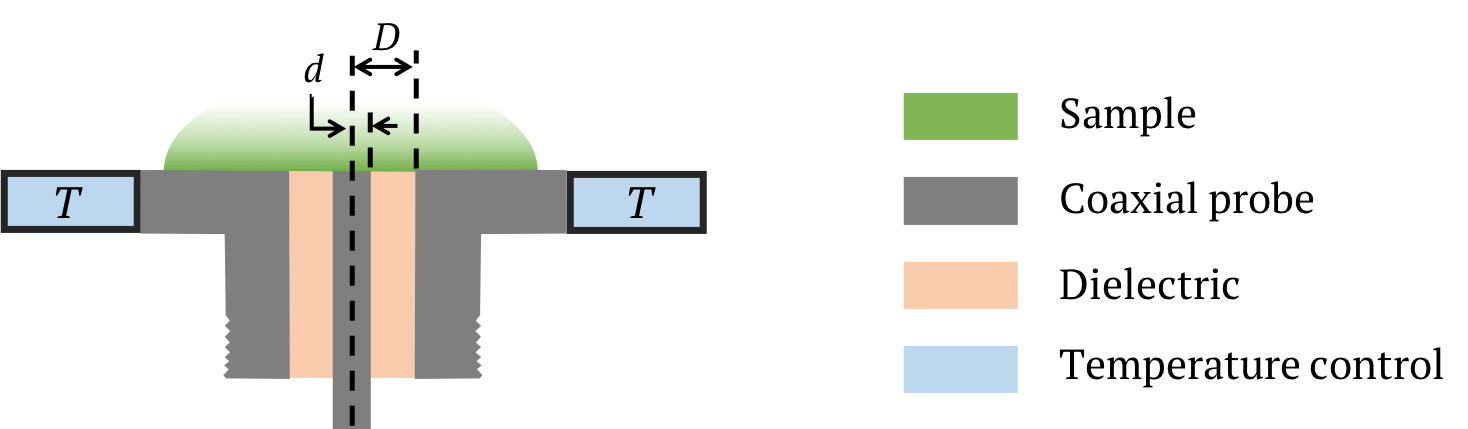
\includegraphics[width=0.8\figwidth]{chapters/Chapter2_Methods/Graphics/SampleCell.png}
	\caption{Transversal cut of the open-ended probe head. The ratio of the incident and the reflected signals at the sample-probe head determines the complex scattering parameter $\hat{S}_r$. The coaxial cable, mentioned in the main text, connects underneath the probe sample cell.}
	\label{SampleCell}
\end{figure}




%Under the knowledge of the probe geometry, a mathematical relation between the complex impedance $\hat{Y}$ and the complex permittivity $\hat{\epsilon}$ can, in principle, be established. Provided with 
For the geometry of the open-ended reflectrometric sample cell, the permittivity-to-impedance relation is given by\!\cite{Blackham1997}
\begin{eqnarray}
\hat{Y} = \frac{ - \hat{k}_s^2}{\pi \hat{k}_c^2 \ln (D/d)} \sum_{n=0}^{\infty} \frac{ (-i)^n \hat{k}_s^{n} I_{n+1}}{n !}
\label{OpenEndedCell}
\end{eqnarray}
\noindent where $D$ and $d$ are the radii of the inner and outer conductors of the coaxial probe, $\hat{k}_c (\omega) = \omega \sqrt{\epsilon_c \epsilon_0 \mu_0}$ is the wavevector of the electric field within the coaxial probe, and $\hat{k}_s (\omega) = \omega \sqrt{\hat{\epsilon}_s \epsilon_0 \mu_0}$ is the wavevector of the electric field in the sample with complex permittivity $\hat{\epsilon} (\omega)$. The coefficients $I_n$ are given by
\begin{eqnarray}
I_n = \int_d^D \int_d^D \int_0^\pi R^{n-2} \cos (\phi) d\phi d r d r' \qquad \text{with} \qquad R^2 = r^2 + r'^2 - 2 r r' \cos (\phi).
\end{eqnarray}



As has been discussed in the original literature for the open-ended sample cell,\!\cite{Blackham1997} the $I_n$ coefficients can be calculated theoretically, but they must be optimized empirically due to the presence of higher order modes of the electric field, which are not included in the derivation of Eq.\ \ref{OpenEndedCell}. The first 40 optimized coefficients $I_n$ have been taken from Johannes Hunger's PhD dissertation,\!\cite{HungerThesis} as have been used for the study of multiple aqueous samples.\!\cite{Hunger2009,Tielrooij2010a,Ensing2013,Ottosson2014c,Cota2018,Smit2019}



Since the sample is located at a certain distance away from the instrument and the setup consist of multiple components, the setup has to be calibrated prior to the measurements. To avoid systematic errors due to imperfections in the electrical network (non-ideal coaxial line), the measured scattering parameter $\hat{S}_{r,m}$ must be corrected to the actual scattering parameter $\hat{S}_{r,a}$ at the probe head according to
\begin{eqnarray}
\hat{S}_{r,m} = \hat{\epsilon}_\lambda + \frac{\hat{\epsilon}_\nu \hat{S}_{r,a}}{1 - \hat{\epsilon}_\sigma \hat{S}_{r,a}},
\label{calibration}
\end{eqnarray}
where $\hat{\epsilon}_\lambda$ accounts for the directional imperfections of the coupling elements, the frequency response $\hat{\epsilon}_\nu$ accounts for changes in the phase that may occur along the finite length of the network, and source match $\hat{\epsilon}_\sigma$ accounts for an impedance mismatch between the the VNA port and the coaxial cable that would lead to re-reflections back to the probe head.



The setup is calibrated by a two-consecutive calibration procedure using three standard references in each step, according to Eq.\ \ref{calibration}. First, the VNA-coaxial cable interface is calibrated via the built-in full-one-port calibration routine using the open, short and match plugs from the ZV-Z218 calibration kit. Second, the interface between the coaxial cable and the sample cell head is calibrated using air (open), conductive silver paint (short) and pure water (match). In all the dielectric relaxation measurements reported in this thesis we employed this calibration routine.



\section{Data analysis and modeling}


Since Eq.\ \ref{OpenEndedCell} has no analytical solution, the complex permittivity is computed numerically via a minimization routine using ``Python'' and the libraries ``Numpy'' and ``Scipy''. These scripts are very extensive to be shown in this thesis, but available at \href{https://github.com/RobertoCota/Dielectric-relaxation-spectroscopy}{https://github.com/RobertoCota/Dielectric-relaxation-spectroscopy}.



The dielectric properties of the solutions studied in this thesis are obtained by means of least-square minimization routines by which the the models discussed in Section \ref{DRTheory} are fitted to the measured dielectric spectra. While the dielectric responses of pure solvents were fitted using a single Debye relaxation mode, the spectra of electrolyte solutions are well described by the sum of a Cole-Cole relaxation mode and a ionic-conductivity term, as expressed in Eq.\ \ref{ColeConRelaxation}. In the lower panel of Figure \ref{RelaxationModes}, the superposed grey lines display the results that best reproduce the experimental data. 



The minimization routine used to determine dielectric properties of electrolyte solutions (as the 1 M \ce{NaCl}:\ce{H2O} in Figure \ref{RelaxationModes}) is shown in Listing \ref{Listing1}.


\newpage


\lstinputlisting[language=Python,caption={Generalized Python script for global analysis in which the real and imaginary components of the complex permittivity are optimized simultaneously.},label={Listing1}]{chapters/Chapter2_Methods/Graphics/OptimizationRoutine.py}







% Add an empty page if needed to accomodate properly the chapter image
%%!TEX root = ../thesis.tex

\chapter*{}
%!TEX root = ../thesis.tex

\thispagestyle{empty}

\begin{tikzpicture}[remember picture,overlay]
\node at (current page.center) {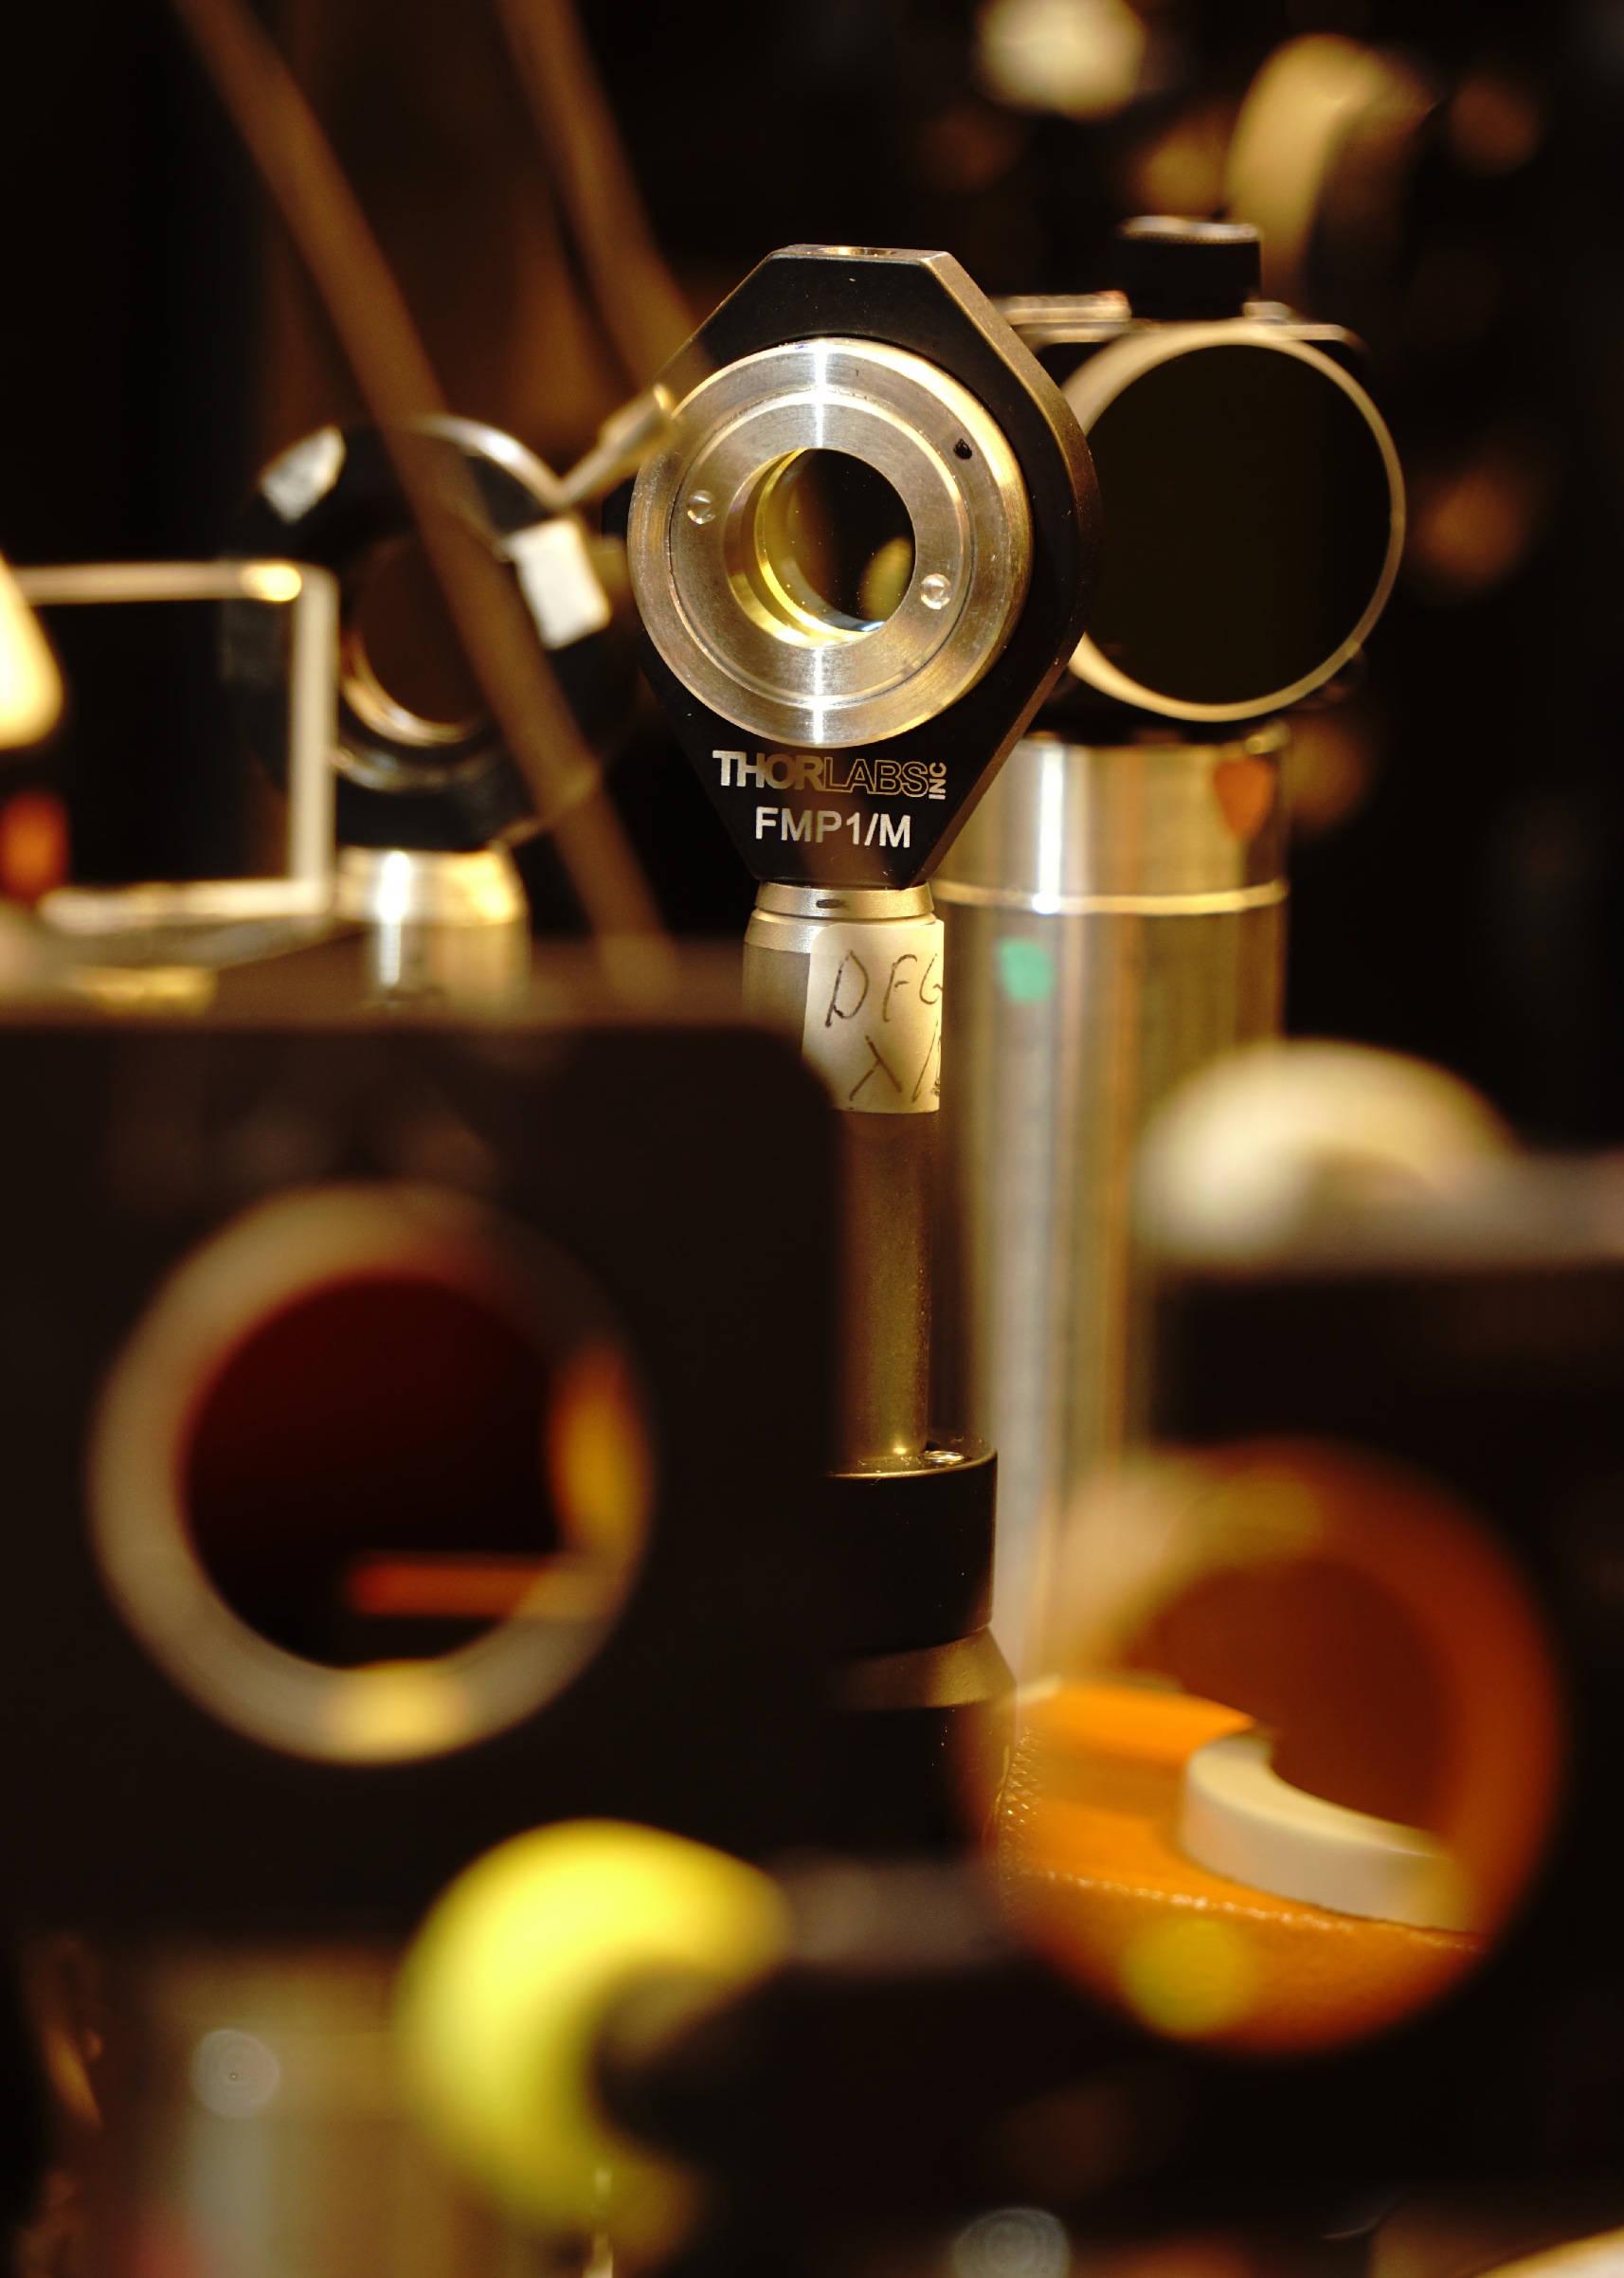
\includegraphics[width=\pdfpagewidth,height=\pdfpageheight]{fullpage_images/OpticsFig.pdf}};
%{\includegraphics[width=\pdfpagewidth,height=\pdfpageheight]{/Users/Cota/Documents/PhD/Thesis/ThesisRoberto/IMG/Chap3.pdf}};
\end{tikzpicture}

\clearpage



\begin{savequote}[75mm]
$\blacktriangleleft$ A \ce{ZnSe} window (the close field orange element in the bottom right) splits our laser pulses into a pump and a probe beam. A halfwave plate (at the focus of the image) enables us to change the polarization of our pump pulses. These two elements set the basis of polarization-resolved pump-probe spectroscopy, leading to a suitable method to observe molecular reorientation.
\end{savequote}




\chapter[Methods II: Vibrational spectroscopy]{Methods II\\Vibrational spectroscopy}
\label{chap:TRVS}
\label{ChapterTRVS}
\label{Chapter3}

\vspace{30pt}
	
	
In this chapter we discuss the theoretical background and experimental methodology used to study aqueous solutions by means of vibrational spectroscopy. In particular, we discuss the aspects that allow light to couple with molecular oscillators and to induce vibrational transitions. By targeting specific vibrational modes, we can then determine the connection between the observable macroscopic properties, such as absorption, and the underlying microscopic structure and dynamics.


\newpage	
	
\section{The classical harmonic oscillator}
	
%Rather than static structures, molecules are regarded as interconnected atoms that are constantly oscillating (small periodical displacements) around the positions that would minimize the internal energy. 
The simplest description of molecular vibrations starts from the classical approach of a diatomic molecule with masses $m$ and $M$ (with $M \gg m$). The two atoms are connected by a covalent chemical bond that acts as a spring, as shown in Figure~\ref{OscillatorsGen1}A. If $m$ experiences a small displacement with respect to its equilibrium position $x_0$ (i.e.\ the equilibrium bond length), the spring exerts a restoring force that follows Hooke's law with a spring constant $k$. Newton's second law states
\begin{eqnarray}
m \frac{d^2 x}{d t^2} + k x = 0,
\end{eqnarray}
with the solution 
\begin{eqnarray}
x (t) = x_0 \cos (\omega_0 t),
\end{eqnarray}
where $\omega_0 = \sqrt{k/m}$ is the frequency at which $m$ oscillates harmonically around its equilibrium position. The preceding equation describes the periodic displacement of $m$ bound to a much heavier atom.

Most molecules consist of more than two atoms. The intramolecular interactions are described as springs pairing all the atoms within the molecule (Fig.\ \ref{OscillatorsGen1}B). This means that the position of a given atom can be affected by multiple bonds, leading to more complex dynamics as compared to the previous example. For a molecule composed of $N$ atoms the equations of motion can be written as
\begin{eqnarray}
M \frac{d^2 X}{d t^2} +  K X = 0,
\label{GeneralizedVibration}
\end{eqnarray}
with $X$ a $3N$-element vector that describes the position of all masses in the three-dimensional space, and $M$ and $K$ matrices ($3N \times 3N$) that contain the corresponding masses $m_i$ and spring constants $k_{ji}$. 

Equation \ref{GeneralizedVibration} constitutes a set of coupled differential equations, which can be solved by a linear transformation to compute the eigenfrequencies of each oscillator in the molecule. We define a unitary matrix $U$ such that
\begin{eqnarray}
(M^{-1} K) U = U \Omega,
\label{EigenFunction1}
\end{eqnarray}
where $\Omega$ is a diagonal matrix that contains the eigenfrequencies $\omega_i$. The unitary matrix can also operate on $X$ to define a new vector as $Q = U^{-1} X$. Hence, Eq.\ \ref{GeneralizedVibration} can be diagonalized, and leads to the equation
\begin{eqnarray}
\frac{d^2 Q}{d t^2} +  \Omega Q = 0,
\label{Diagonalsolution}
\end{eqnarray}
that provides a set of $3N$ uncoupled differential equations. Hence, the oscillating dynamics of atoms within the molecule are described by superposition of independent harmonic oscillators $q_i$, conventionally called ``normal modes''.



\begin{figure}[t!]
	\centering
	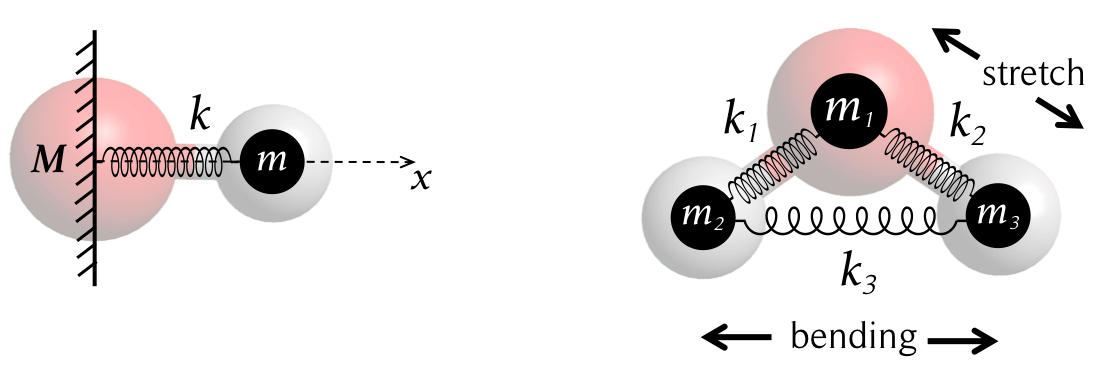
\includegraphics[width=0.85\figwidth]{chapters/Chapter3_Methods2/Graphs/Oscillators.png} %The local modes are calculated on the XXX level, and reproduced with permission from ref. XXX. 
	\caption{\textbf{Left:} Covalent chemical bonds can be modeled as harmonic oscillators. \textbf{Right:} Representation of a polyatomic molecule (water) with respect of its different degrees of vibrational freedom.}
	\label{OscillatorsGen1}
\end{figure}




Water molecules are formed by three atoms with two non-parallel covalent bonds, so water has three normal modes (see Fig.\ \ref{OscillatorsGen1}B): a bending mode, and two \ce{OH} stretches that combine to give the symmetric and antisymmetric stretch modes.\!\cite{Wang2004,Bakker2010,Perakis2016}



\section{Quantum description and vibrational transitions}


In the quantum mechanical description of molecular vibrations, we again describe chemical bonds as harmonic oscillators, leading to the following Hamiltonian:
\begin{eqnarray}
\hat{H}_0 = \frac{\hat{p}^2}{2m} + \frac{1}{2} k \hat{x}^2,
\label{SchodringerStatic}
\end{eqnarray} 
where $\hat{p}$ ($= -i \hslash \partial_x$) and $\hat{x}$ are the momentum and position operators. The first term represents the kinetic energy of the system, while the second corresponds to the potential energy of a particle in a Hooke's law-type potential. 

Solving the time-independent Schr\"odinger equation $\hat{H}_0 \ket{\Psi} = E \ket{\Psi}$ yields a family of solutions defined by the following orthogonal eigenstates 
\begin{eqnarray}
\ket{\psi_n (x)}=\frac{1}{\sqrt{2^{n} n !}} \cdot \left(\frac{m \omega_0}{\pi \hslash}\right)^{1 / 4} \cdot \exp \left(  {-\frac{ m \omega_0 x^{2}}{2 \hslash}}  \right) \cdot H_{n}\left(\sqrt{\frac{m \omega_0}{\hslash}} x \right),
\label{wavefunctions}
\end{eqnarray} 
with $\ket{\psi_{n}}$ the stationary wavefunctions that obey the relation $\braket{\psi_n}{\psi_m} = \delta_{nm}$, with $\delta_{nm}$ the Kronecker delta, and $H_n$ the Hermite polynomials. The corresponding eigenenergies are given by
\begin{eqnarray}
E_n = \hslash \omega_0 \left( n + \frac{1}{2}   \right), \qquad \text{with} \qquad n \in \mathbb{N}_0.
\label{eigenenergy}
\end{eqnarray}
\begin{figure}[t!]
	\centering
	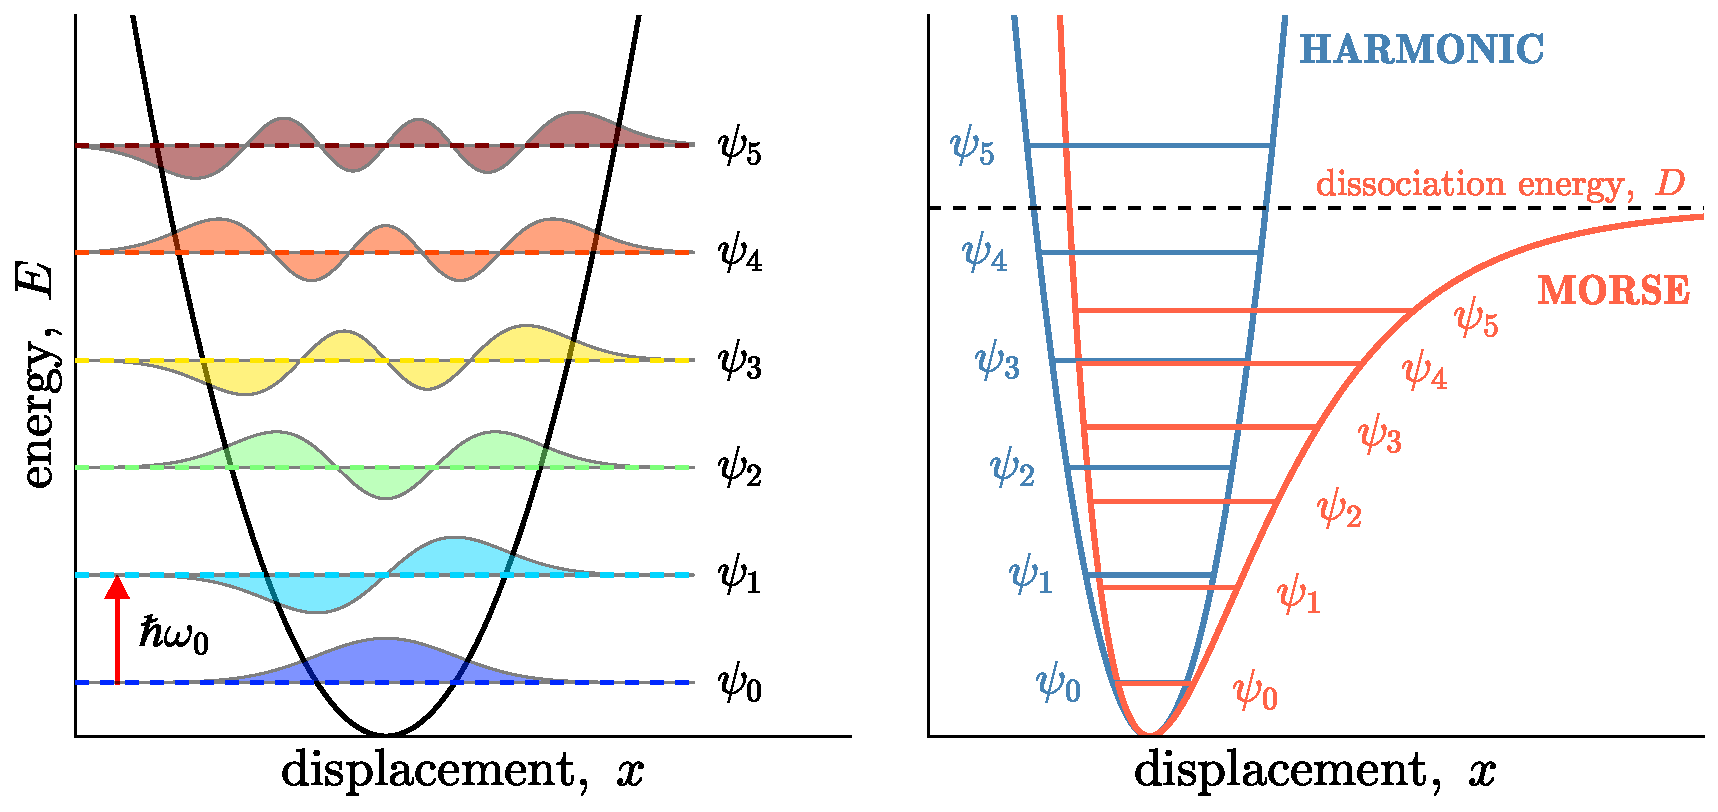
\includegraphics[width=1\figwidth]{chapters/Chapter3_Methods2/Graphs/PotentialHarmonicMorse.pdf} %The local modes are calculated on the XXX level, and reproduced with permission from ref. XXX. 
	\caption{\textbf{Left:} Wavefunctions described in a harmonic oscillator potential. Each wavefunction is drawn at its corresponding energy level. Consecutive level are equidistant by a quanta of energy $\hslash \omega_0$. \textbf{Right:} Comparison between the harmonic oscillator potential and anharmonic vibrations described by the Morse potential. Notice that the latter has a asymptotic behavior at large distances, which corresponds to the dissociation energy level. In the Morse potential, the space between consecutive energy levels decreases with increasing the quantum number $n$.}
	\label{PotentialsWaveFunctions}
\end{figure}

The value $n$ corresponds to the vibrational quantum number, and $\omega_0 = \sqrt{k/m}$. Eqs.\ \ref{wavefunctions} and \ref{eigenenergy} state that the energy is quantized and the system can only be in discrete states, referred to as zeroth, first, second and higher order vibrational states, shown in the left panel of Fig. \ref{PotentialsWaveFunctions}. From Eq.\ \ref{eigenenergy}, it is clear that the energy of the ground state ($n=0$) is not zero, but $E_0 = \hslash \omega_0 /2$ which is called the zero-point energy. Subsequent states are equidistantly separated by a quantum of energy $\hslash \omega_0$. 


%The discrete character of  contrast with the classical oscillator in which the ground state coincides with the static non-oscillating dynamics.





In the quantum description, transitions between levels can occur as the result of a time-dependent perturbation, such as light (electromagnetic waves). As shown in Eq.\ \ref{PotentialPolarization}, an electromagnetic wave interacts with the charges in the system, adding a new term to the Hamiltonian:
\begin{eqnarray}
\hat{H} = \hat{H}_0 + \hat{V}_\text{int}(t), \qquad \text{with} \qquad \hat{V}_\text{int}(t) = \hat{\vec{\mu}} \cdot \vec{E}(t),
\label{PerturbedHamiltonian}
\end{eqnarray} 
where $\vec{E}(t)$ refers to the electric field of the light and the dipole moment operator $\hat{\vec{\mu}}$ defines the distribution of charges $q$ in the system following $\hat{\vec{\mu}} = \sum_i q_i \hat{\vec{x}}_i$.


A transition from a vibrational level to another can be described using the time-dependent Schr\"odinger equation
\begin{eqnarray}
\hat{H} (t) \ket{\Psi} = i \hslash \frac{\partial}{\partial t} \ket{\Psi},
\label{TimeScrodinger}
\end{eqnarray} 
which can be solved by separation of variables. Using the expressions given by Eqs.\ \ref{wavefunctions} and \ref{eigenenergy}, the general solution to Eq.\ \ref{TimeScrodinger} is written as
\begin{eqnarray}
\ket{\Psi} = \sum_n c_n (t)  e^{  -i E_n t / \hslash  } \ket{\psi_n}
\label{GenSolTimeSchrodinger}
\end{eqnarray}
where $c_n (t)$ is the corresponding amplitude of each energy level at time $t$.


% and the probability of finding the system in any state $\ket{\psi_n}$ is found by evaluating
%the superposition of the different vibrational states given in Eq.\  and the different eigenenergies from Eq. , thus


Using Eqs.\ \ref{PerturbedHamiltonian}, \ref{TimeScrodinger} and \ref{GenSolTimeSchrodinger}, the time-dependent amplitude of a given $\ket{\psi_m}$ state can be computed as follows
\begin{eqnarray}
\frac{d }{d t} c_m (t) = \frac{1}{i \hslash} \sum_n c_n (t) \bra{\psi_m} \hat{V}_\text{int} \ket{\psi_n} e^{-i \omega_{nm} t},
\label{TransitionPsi}
\end{eqnarray}
where $\omega_{nm} = (E_n - E_m) / \hslash = - \omega_{mn}$ is the energy difference between the states $n$ and $m$. The preceding equation provides a full description of the population of the state $m$, although not practical because each unknown coefficient $c_m$ is determined by the whole set of $c_n$ coefficients. Assuming that the system is entirely in a single state $k$ at $t = 0$ and the initial state is negligibly perturbed over the time, meaning $c_k(0) = 1$ and $c_k(t) \simeq 1$, Eq.\ \ref{TransitionPsi} reduces to\!\cite{Sakurai1994}
\begin{eqnarray}
c_m (t) \simeq \frac{1}{i \hslash} \int_0^t \bra{\psi_m} \hat{V}_\text{int} (t') \ket{\psi_k} e^{-i \omega_{km} t'}.
\label{TransitionPsi2}
\end{eqnarray}

The simplest description of such perturbation is to assume a harmonically oscillating electric field (harmonic perturbation) as $\vec{E} = \vec{E}_0 [\exp(i \omega t) + \exp(-i \omega t)]$. In that case, the transition rate $\Gamma_{k \to m}$, that is defined as the time derivative of the square modulus of $c_m$, is given by 
\begin{eqnarray}
\Gamma_{k \to m} \simeq \frac{d}{d t} | c_m |^2 &=& \frac{2 \pi}{ \hslash^2} |   \bra{\psi_m} \hat{\vec{\mu}} \cdot \vec{E}_0 \ket{\psi_k}   |^2 \delta(  \omega \pm \omega_{km}), \nonumber \\
&=& \frac{2 \pi}{ \hslash^2} E_0^2 \cos^2 (\theta) |   \bra{\psi_m} \hat{\mu}  \ket{\psi_k}   |^2  \delta(\omega \pm \omega_{km} ),
\label{TransRate}
\end{eqnarray}
which is the so-called Fermi's golden rule, where $\theta$ defines the angle between the dipole moment and the polarization of the perturbing electric field. The expression $ \mu_{mk} = \bra{\psi_m} \hat{\mu}  \ket{\psi_k}$ is generally called transition dipole moment. In the last expression, the dipole operator $\hat{\mu}$ refers to the entire distribution of charges, which encompasses transition dipoles of any kind. In the case of vibrational transitions, the transition dipole operator can be written in terms of the oscillation coordinate $x$ and the equilibrium position $x_0$ by the following expansion
\begin{eqnarray}
\hat{\mu} = {\mu}_0 + \frac{d {\mu}}{ d x} (\hat{x} - {x}_0) + \cdots
\end{eqnarray}
which leads to 
\begin{eqnarray}
\Gamma_{k \to m} = \frac{2 \pi}{ \hslash^2} E_0^2 \cos^2 (\theta) \left( \frac{d \mu}{d x}   \right)^2 |   \bra{\psi_m} \hat{x}  \ket{\psi_k}   |^2  \delta(\omega \pm \omega_{km} ).
\label{TransRateFinal}
\end{eqnarray}

This equation has the following physical interpretation: 

\begin{itemize}
	\item {The $\delta(\omega \pm \omega_{km})$ term represents the conservation of energy in the transition $\ket{\psi_k} \to \ket{\psi_m}$. We see that such condition can only be satisfied either by energy taken away from the external electric field (absorption if $E_m \simeq E_k + \hslash \omega$) or by energy given out to the external electric field (stimulated emission if $E_m \simeq E_k - \hslash \omega$). In both cases, such transition takes place when $\omega$ matches the energy difference between the states $m$ and $k$ (see Fig.\ \ref{dia2})}.
	\item {The $\bra{\psi_m} \hat{x}  \ket{\psi_k} $ term establishes the transition selection rule since it is zero unless $m = k \pm 1$, meaning that transitions only occur between consecutive states.\!\cite{Sakurai1994}}
\end{itemize}
	\begin{figure}[t!]%* is used because without it the figure does not appear
		\centering	
		\begin{tikzpicture}[>=stealth,thick,photon/.style={decorate,decoration={snake,post length=1.3mm}}]	
		
	
		\draw[->, line width=0.6mm, ForestGreens] (4.4-4,2.4) -- (4.4-4,4.0);		
		
		\draw[black,line width=0.7mm](3.8-4,4.0) -- (5-4,4.0) node[right] {$\ket{\psi_{n+1}}$};
		\draw[black,line width=0.7mm](3.8-4,2.4) -- (5-4,2.4) node[right] {$\ket{\psi_{n}}$};
				
		\draw[->,photon, line width=0.4mm, red] (2.9-4,3.2) -- (4.3-4,3.2) node[pos=0.2, above] {$\hslash \omega_0$};

		
		
		
		
		\draw[->, line width=0.6mm, blue] (4.4,4.0) -- (4.4,2.4);		
		
		\draw[black,line width=0.7mm](3.8,4.0) -- (5,4.0) node[right] {$\ket{\psi_{n+1}}$};
		\draw[black,line width=0.7mm](3.8,2.4) -- (5,2.4) node[right] {$\ket{\psi_{n}}$};
		
		\draw[->,photon, line width=0.4mm, red] (2.9,3.2) -- (4.3,3.2) node[pos=0.2, above] {$\hslash \omega_0$};
		
		\draw[->,photon, line width=0.4mm, red] (4.6,3.4) -- (6.0,3.4) node[pos=0.2, above] {$\hslash \omega_0$};	
		
		\draw[->,photon, line width=0.4mm, red] (4.6,3.0) -- (6.0,3.0) node[pos=0.2, below] {$\hslash \omega_0$};
		
			
			
			
		\draw[->, photon, line width=0.5mm, MyYellow] (4.4+4,4.0) -- (4.4+4,2.4);			
			
		\draw[black,line width=0.7mm](3.8+4,4.0) -- (5+4,4.0) node[right] {$\ket{\psi_{n+1}}$};
		\draw[black,line width=0.7mm](3.8+4,2.4) -- (5+4,2.4) node[right] {$\ket{\psi_{n}}$};
		
		%\draw[->,photon, line width=0.4mm, red] (4.6+4,3.2) -- (6.0+4,3.2) node[pos=0.2, above] {$\hslash \omega_0$};	
		
%		\draw[black,line width=1.2mm](3.5,1.0) -- (5.0,1.0) node[pos=0.5,below] {hot ground state};
		
%		\draw[black,line width=1.2mm] (1,0.2) -- (7,0.2) node[pos=0.15,above] {ground state};
		
		
		\node[right,fill=white,opacity=.2,text opacity=1,align=left] at (3.5-4,1.625) {$\text{absorption}$};
		
		\node[right,fill=white,opacity=.2,text opacity=1,align=left] at (3.5,1.8) {$\text{stimulated}$};
		\node[right,fill=white,opacity=.2,text opacity=1,align=left] at (3.65,1.45) {$\text{emission}$};
		
		\node[right,fill=white,opacity=.2,text opacity=1,align=left] at (3.4+4,1.8) {$\text{spontaneous}$};
		\node[right,fill=white,opacity=.2,text opacity=1,align=left] at (3.8+4,1.45) {$\text{decay}$};

		
%		\draw[white,line width=0.05mm](1,-0.1) -- (7,-0.1);
		
		
		\end{tikzpicture}		
		\caption{Illustration for three different transition processes: absorption, stimulated emission and spontaneous decay. The illustration pictures the ideal case in which the energy of the photon matches the energy difference between two consecutive states.}
		\label{dia2}			
	\end{figure}
\begin{itemize}
	\item {The $d \mu / d x$ term implies that the external electric field only couples to those vibrations that induce changes in the dipole moment.}
	\item {From the term $\cos^2 (\theta)$, we observe that the probability of a $\ket{\psi_k} \to \ket{\psi_m}$ transition to occur depends on the angle between the transition dipole moment and the polarization of the external electric field. This probability is maximal at $\theta = 0$, which means $ \vec{\mu} \parallel \vec{E}_0$. This is the basis of polarization-resolved spectroscopy which we will discuss later.}
\end{itemize}


In real molecules, the potential cannot be quadratic due to molecular dissociation at large interatomic distances.\!\cite{Maksyutenko2012} A more adequate potential to include the effect of molecular dissociation is given by
\begin{eqnarray}
V_\text{M} (x) = D \left( 1 - e^{-a x}   \right)^2,
\label{MorsePotential}
\end{eqnarray}
the so-called Morse potential,\!\cite{Morse1929} shown in the right panel of Figure~\ref{PotentialsWaveFunctions}. The energy at which the bond dissociates is represented by $D$, and $a = \sqrt{k/2D}$ the width of the potential. By introducing Eq.\ \ref{MorsePotential} in Eq.\ \ref{SchodringerStatic} instead of the harmonic oscillator potential, the corresponding eigenenergies related to the Morse potential are expressed as follows
\begin{eqnarray}
E_n = \hslash \omega_0 \left( n + \frac{1}{2}   \right) - \frac{\hslash^2 \omega_0^2}{4 D} \left( n + \frac{1}{2}   \right)^2,
\label{MorseEnergies}
\end{eqnarray}
where $n$ again is the vibrational quantum number and the angular frequency $\omega_0$ ($= \sqrt{k/m}$) satisfies also the relation $ \omega_0 = a \sqrt{2 D/ m}$. In contrast to the description of an harmonic oscillator, the energy separation between consecutive states becomes smaller with increasing the quantum number $n$. At low $n$, Eq.\ \ref{MorseEnergies} can be well represented by Eq.\ \ref{eigenenergy}. Further potentials have been explored to overcome some limitations of the Morse potential, such as the long-range Morse potential that captures the attractive long-range behavior in real systems.\!\cite{LeRoy2009}





\section{Linear absorption spectroscopy}


The way in which light interacts with an absorbing medium can give information at the molecular level. As in the previous chapter, to describe the vibrational experiments we need to construct models based on the changes that an incident field (light) experiences as it propagates through a medium. 

Assume a system of molecular oscillators of the same species in thermal equilibrium, meaning that the system is isotropic and in the ground state $\ket{0}$, so absorption is the most likely process to occur in the presence of light. This process will lead to attenuation of the incident field and non-zero, but relatively small, population of the first excited state $\ket{1}$.

For monochromatic light with intensity of $I_0 = c \epsilon_0 |E_0|^2 /2$ and frequency $\omega$, the absorbed power associated with the $\ket{0} \to \ket{1}$ transition is written as $P_\text{01} = \hslash \omega \Gamma_{0 \to 1}$. The absorption cross section $\sigma_\text{10}$ is defined as the ratio between the latter expressions, and using Eq.\ \ref{TransRateFinal}, is given by
\begin{eqnarray}
\sigma_\text{10} (\omega) = \frac{P_\text{10} (\omega) }{I_0} =  \frac{\pi \omega }{3 c \epsilon_0 \hslash } \mu_{10} \delta(\omega \pm \omega_{10})
\label{crosssection}
\end{eqnarray}
in which $\langle cos^2 \theta \rangle = 1/3 $ since the material is assumed isotropic. The cross section can be understood as an effective transverse area (not necessarily linked to the dimensions of the molecule) that the incident field must hit in order for the given transition to occur.

Assume now that a field propagates in the $z$ direction through a material with thickness $L$ and density of oscillators in the ground state $\rho$ (Fig.\ \ref{AbsorptionLambertBeer}), the Lambert-Beer law
\begin{eqnarray}
d I = - \sigma_\text{10} (\omega) \rho I {d z}
\label{lambertbeerlaw}
\end{eqnarray}
states that the variation of intensity $d I$ through propagation in a segment $dz$ is equal to the product between the intensity and the cross section of the material. Integrating this expression gives
\begin{eqnarray}
I = I_0 \exp [- \beta (\omega) L ],
\label{lambertbeerlaw2}
\end{eqnarray}
\begin{figure}[t!]
	\centering
	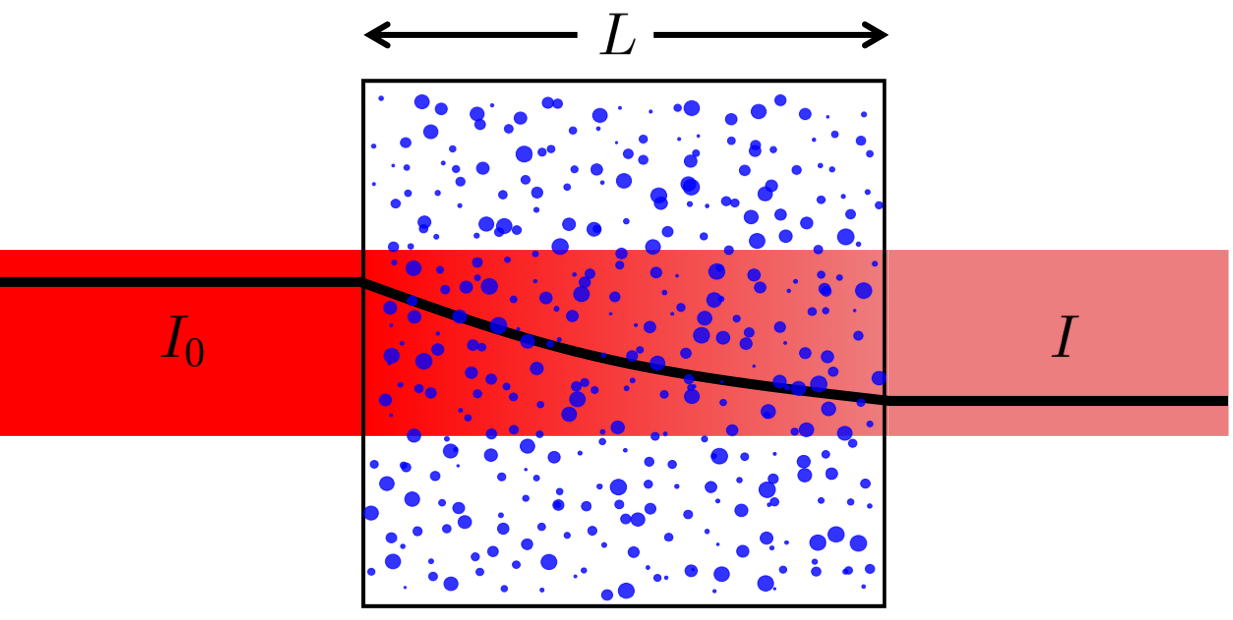
\includegraphics[width=0.6\figwidth]{chapters/Chapter3_Methods2/Graphs/LambertBeerAbs.png} %The local modes are calculated on the XXX level, and reproduced with permission from ref. XXX. 
	\caption{In linear absorption spectroscopy, one studies the decrement on the intensity of light as it propagates through a material. The initial and the final intensities are linked by the spectroscopic properties of the sample as described by Eqs.\ \ref{crosssection} and \ref{lambertbeerlaw2}.}
	\label{AbsorptionLambertBeer}
\end{figure}
\noindent with $\beta (\omega) = \rho \sigma_\text{10} (\omega)$ the attenuation coefficient. This equation provides a link between the macroscopic transmission of the material, $T = I/I_o$, with the microscopic molecular property $\sigma_{10}$. The absorbance, which provides a more convenient and linear relation between the relevant parameters, is given by
\begin{eqnarray}
\alpha (\omega) = - \ln \frac{I}{I_0} = \sigma_{10} (\omega) \rho L.
\label{absorbance}
\end{eqnarray}




As can be observed from Eq.\ \ref{crosssection}, a vibrational transition will only occur when the frequency of the electric field matches the energy difference between the excited and ground states. 


In condensed-phase systems, the absorption spectrum $\alpha(\omega)$ is not a delta function as it would result from Eqs.\ \ref{crosssection} and \ref{absorbance}, but has a finite width. This is due to two effects. First, the finite excited-state lifetime and fast fluctuations in the resonance frequency (due to interaction of the oscillator with its surroundings) give rise to so-called homogeneous broadening. This broadening occurs for each individual oscillator, and if all oscillators have the same resonance frequency $\omega_{10}$, it typically gives rise to a Lorentzian line shape:
\begin{eqnarray}
I (\omega ) \propto \frac{1}{\pi} \frac{\gamma/2}{ (\omega - \omega_{10})^2 + (\gamma/2)^2},
\label{Lorentzian}
\end{eqnarray}
where $\gamma$ is the homogeneous line width (see Fig.\ \ref{BroadeningFigure1}-left). In addition, there may exist a distribution of resonance frequencies $\omega_{10}$ in the sample, so that the absorption spectrum becomes the convolution of Eq.\ \ref{Lorentzian} with this distribution of resonance frequencies (see Fig.\ \ref{BroadeningFigure1}-right). This so-called inhomogeneous broadening occurs very often in hydrogen-bonded systems, where local differences in hydrogen-bond strength give rise to a broad distribution of \ce{OH}- or \ce{OD}-stretch frequencies (see Chapters \ref{ChapterHydroxide}, \ref{ChapterForster} and \ref{ChapterPhenolate}).



\begin{figure}[t!]
	\centering
	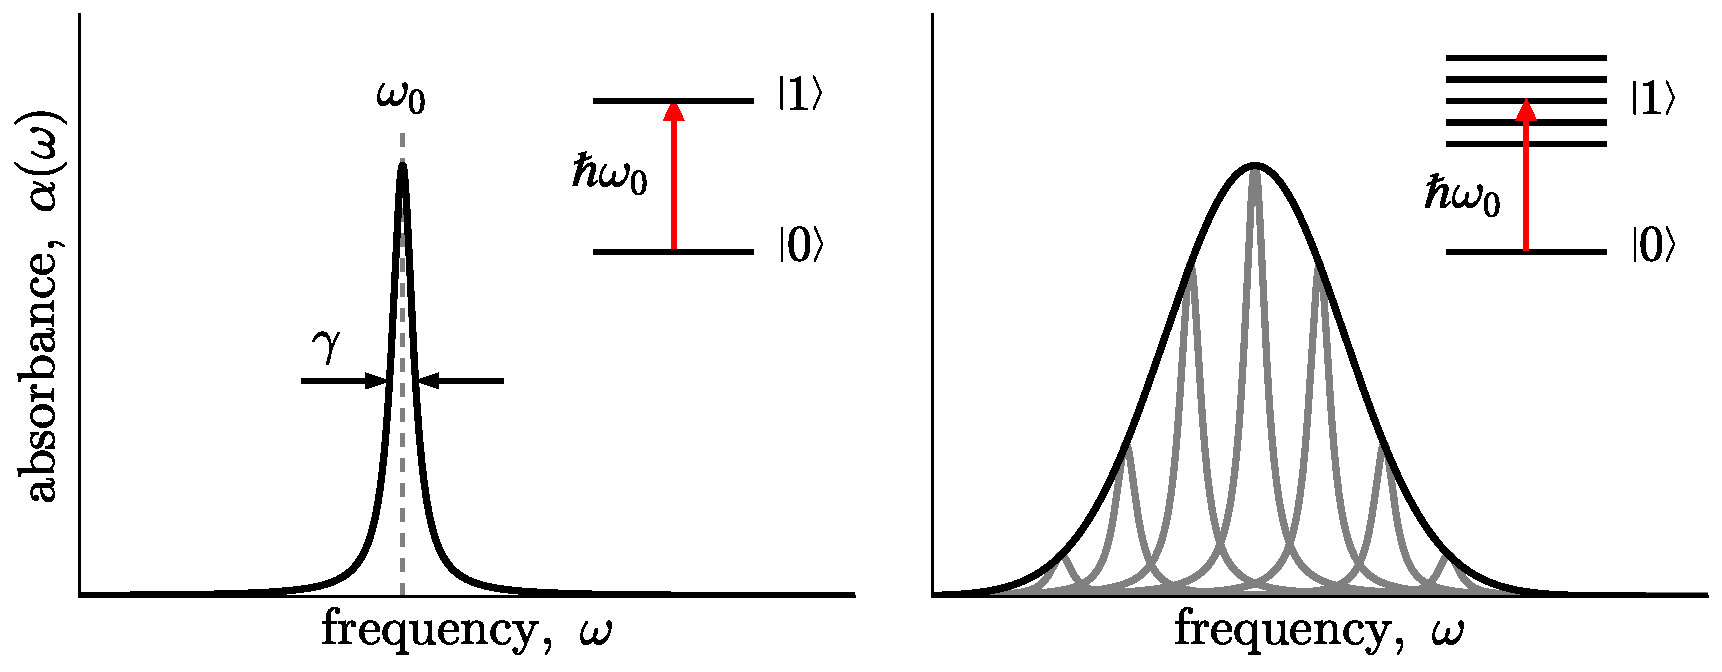
\includegraphics[width=0.95\figwidth]{chapters/Chapter3_Methods2/Graphs/LineShape.pdf} %The local modes are calculated on the XXX level, and reproduced with permission from ref. XXX. 
	\caption{\textbf{Left:} homogeneous broadening due to the finite lifetime of the excited state and fast fluctuations of the resonance frequency. This effect follows a Lorentzian functional form.  \textbf{Right:} the absorption lineshape is further broadened due to intermolecular interactions such as hydrogen bonding, leading to a statistical distribution of the resonance frequency.}
	\label{BroadeningFigure1}
\end{figure}





\section{Time-resolved vibrational spectroscopy}\label{TRVSExp}

Pump-probe spectroscopy is a useful tool to study dynamical aspects of molecular systems. This technique is based on an intense pulse that excites a significant fraction of the oscillators contained in a sample to the excited state (pump), while a second time-delayed weak pulse monitors the equilibration mechanism of the excited oscillators (probe). The pump and probe processes are shown in Figure~\ref{excitationscheme}.


\begin{figure}[t!]%* is used because without it the figure does not appear
	\centering	
	\begin{tikzpicture}[>=stealth,thick,photon/.style={decorate,decoration={snake,post length=1.3mm}}]	
	
	
	\draw[black,line width=0.6mm](3-6,5.0) -- (4.9-6,5.0) node[right] {$\ket{2}$};
	\draw[black,line width=0.6mm](3-6,4.0) -- (4.9-6,4.0) node[right] {$\ket{1}$};
	\draw[black,line width=0.6mm](3-6,2.7) -- (4.9-6,2.7) node[right] {$\ket{0}$};
	
	
	\draw[->, line width=0.6mm, ForestGreens] (3.7-6,2.7) -- (3.7-6,4.0);
	\draw[->, line width=0.6mm, ForestGreens] (4.2-6,2.7) -- (4.2-6,4.0);
	\draw[->, line width=0.6mm, ForestGreens] (4.45-6,2.7) -- (4.45-6,4.0);	
	
	
	\filldraw[gray] (3.2-6,2.7) circle (3pt);
	\filldraw[gray] (3.45-6,2.7) circle (3pt);	
	\filldraw[gray] (3.7-6,2.7) circle (3pt);	
	\filldraw[gray] (3.95-6,2.7) circle (3pt);	
	\filldraw[gray] (4.2-6,2.7) circle (3pt);	
	\filldraw[gray] (4.45-6,2.7) circle (3pt);	
	\filldraw[gray] (4.7-6,2.7) circle (3pt);	
	
	
	\draw[->,photon, line width=0.4mm, red] (1.2-6,4.7) -- (2.6-6,4.2);
	
	\draw[->,photon, line width=0.4mm, red] (1.2-6,4.4) -- (2.6-6,3.9);	
	
	\draw[->,photon, line width=0.4mm, red] (1.2-6,4.1) -- (2.6-6,3.6);
	
	\node[right,fill=white,opacity=.2,text opacity=1,align=left] at (1.3-6,3.3) {$\text{pump}$};
	
	
	
	
	
	\draw[black,line width=0.6mm](3,5.0) -- (4.9,5.0) node[right] {$\ket{2}$};
	\draw[black,line width=0.6mm](3,4.0) -- (4.9,4.0) node[right] {$\ket{1}$};
	\draw[black,line width=0.6mm](3,2.7) -- (4.9,2.7) node[right] {$\ket{0}$};
	
	\draw[->, line width=0.6mm, ForestGreens] (3.45,2.7) -- (3.45,4.0);
	\draw[->, line width=0.6mm, ForestGreens] (3.7,4.0) -- (3.7,5.0);
	\draw[->, line width=0.6mm, blue] (4.2,4.0) -- (4.2,2.71);	
	
	
	\filldraw[gray] (3.2,2.7) circle (3pt);
	\filldraw[gray] (3.45,2.7) circle (3pt);	
	\filldraw[gray] (3.7,4.0) circle (3pt);	
	\filldraw[gray] (3.95,2.7) circle (3pt);	
	\filldraw[gray] (4.2,4.0) circle (3pt);	
	\filldraw[gray] (4.45,4.0) circle (3pt);	
	\filldraw[gray] (4.7,2.7) circle (3pt);	
	
	%	\draw[->,photon, line width=0.4mm, red] (1.2,4.7) -- (2.6,4.2);
	
	\draw[->,photon, line width=0.4mm, red] (1.2,4.4) -- (2.6,3.9);	
	
	%	\draw[->,photon, line width=0.4mm, red] (1.2,4.1) -- (2.6,3.6);
	
	\node[right,fill=white,opacity=.2,text opacity=1,align=left] at (1.3,3.6) {$\text{probe}$};
	
	\end{tikzpicture}		
	\caption{Illustration of pump-probe spectroscopy in which the first three vibrational states are considered. The gray circles represent population. \textbf{Left:} at $t = 0$, an intense pump beam promotes vibrations to the first excited state (green arrows), which are after monitored by a second beam called probe. \textbf{Right:} the probe induces three different effects: excitation from ground to the first excited state, excitation from the first to the second excited state, and stimulated emission from the first to the ground state.}
	\label{excitationscheme}			
\end{figure}


Here, we aim to provide a phenomenological understanding behind pump-probe spectroscopy. To this purpose, we start with the notion of transient absorption which arises from the difference between the absorption of the perturbed sample and of the unperturbed sample. The system is perturbed out of its equilibrium due to te intense pump pulse. The transient absorption is defined as
\begin{eqnarray}
\Delta \alpha (\omega,t) = \alpha_\text{p} (\omega,t) - \alpha_\text{u}(\omega),
\label{transientspectra1}
\end{eqnarray} 
where the subindices $p$ and $u$ refer to the pumped and the unpumped sample. As shown in Eq.\ \ref{absorbance}, the absorbance of the unpumped sample is given by
\begin{eqnarray}
\alpha_\text{u} (\omega) = \sigma_{01} (\omega) N_0
\end{eqnarray}
with $N_0 = \rho L$ the number of vibrational absorbers per area unit in the ground state. After excitation by the pump pulse, the prope pulse will experience a change in the absorption as the result of three different processes. First, the density of absorbers in the ground state is reduced, such that the $\ket{0} \to \ket{1}$ absorption is reduced by a factor of $(N_0-N_1(t))/N_0$, with $N_1(t)$ the density of molecules in the excited state at any time. A second effect is stimulated emission that also manifests itself as an increase in the transmission of the sample, in other words, a reduced absorbance according to Eq.\ \ref{absorbance}. Third, the probe pulse can promote molecules from the first to the second excited state which induces an absorption matching the $\ket{1} \to \ket{2}$ transition. These effects can be represented as follows
\begin{eqnarray}
\alpha_\text{p} (\omega,t) = \underbrace{\sigma_{10} (\omega) [N_0 - N_1(t)]}_{\text{ground state} \atop \text{depletion}}  - \underbrace{\sigma_{01} (\omega) N_1(t)}_{\text{stimulated} \atop \text{emission}} + \underbrace{\sigma_{21} (\omega) N_1 (t)}_{\text{induced} \atop \text{absorption}}.
\end{eqnarray}
Since $\sigma_{10} = \sigma_{01}$, the transient absorption change defined in Eq.\ \ref{transientspectra1} reduces to
\begin{eqnarray}
\Delta \alpha (\omega,t) = - \underbrace{ 2 \sigma_{10} (\omega) N_1(t)}_{\text{bleaching} \atop \text{band}} + \underbrace{\sigma_{21} (\omega) N_1 (t)}_{\text{induced} \atop \text{absorption}}, 
\label{transientabs2}
\end{eqnarray}
with features that are represented in the left side of Figure~\ref{TRVSAspects1} (for short time delays).


\begin{figure}[t!]
	\centering
	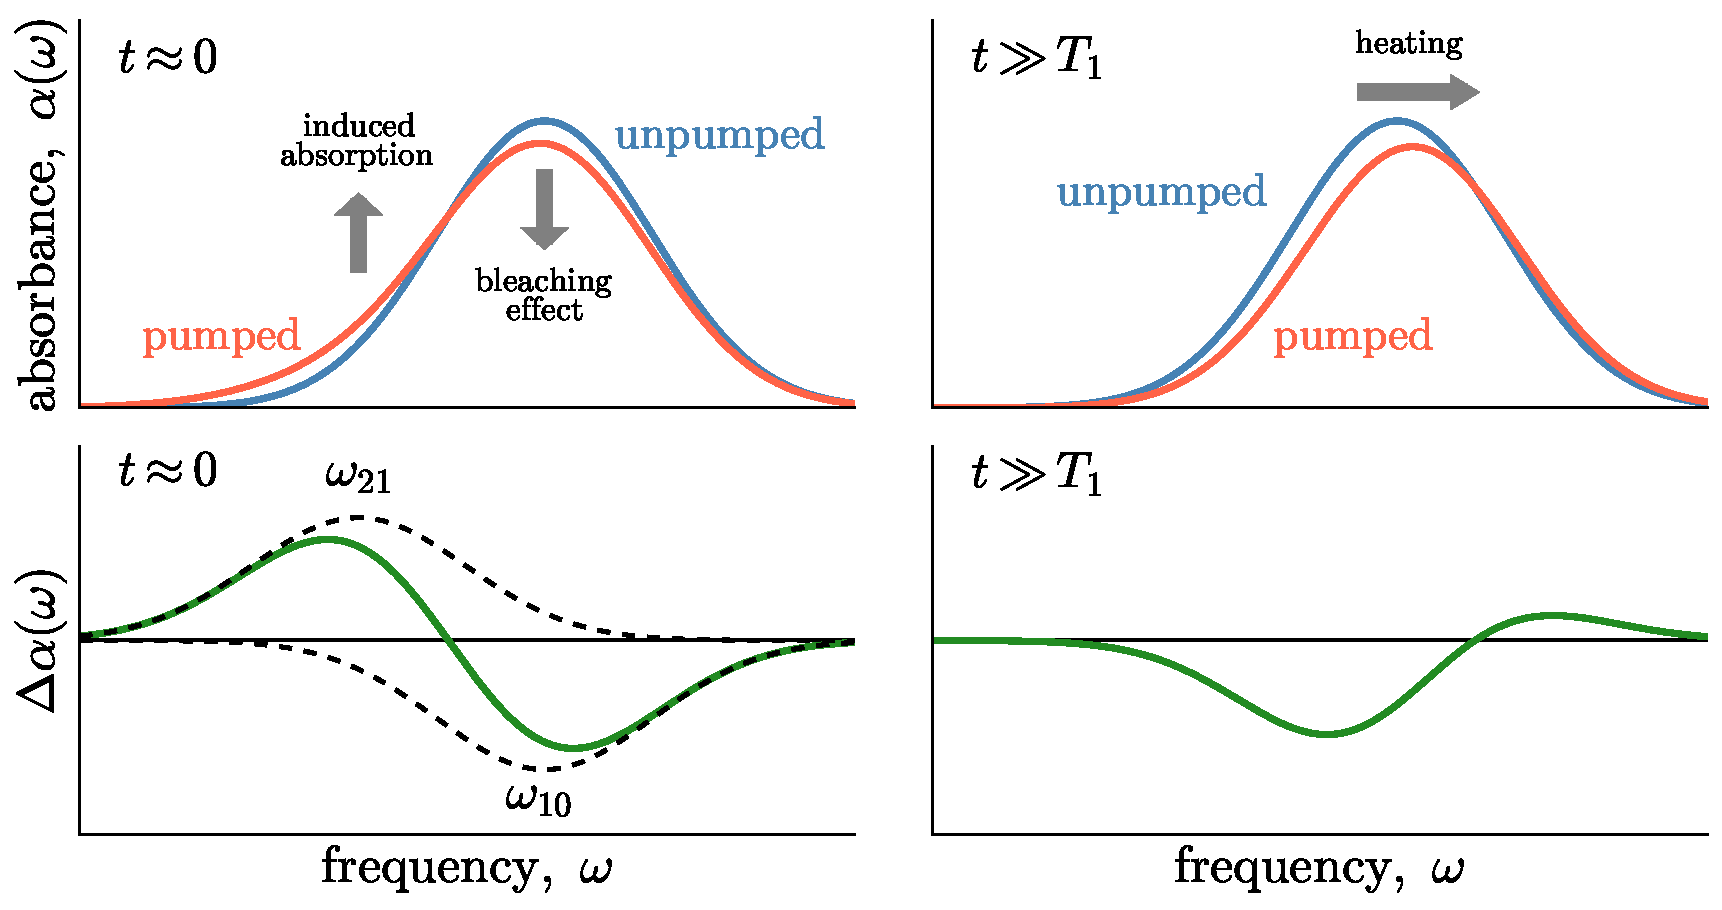
\includegraphics[width=0.95\figwidth]{chapters/Chapter3_Methods2/Graphs/TRVSAspects.pdf} %The local modes are calculated on the XXX level, and reproduced with permission from ref. XXX. 
	\caption{Illustration of pump-probe spectra that resemble the response of the \ce{OD} stretch vibration of \ce{HDO} molecules isotopically diluted in \ce{H2O}. \textbf{Left:} at short time delays the absorption is reduced around $\omega_{10}$ (bleaching), while absorption around $\omega_{21}$ is accessible. \textbf{Right:} at long time delays the absorption spectrum shifts to the blue and reduces in amplitude due to temperature increase upon vibrational relaxation.}
	\label{TRVSAspects1}
\end{figure}



In the simplest scenario, the excited molecules decay directly to the ground state, so that the bleaching and induced absorption vanish exponentially in the same fashion, such that
\begin{eqnarray}
\Delta \alpha (\omega,t) = [ -  2 \sigma_{10} (\omega) + \sigma_{21}(\omega)] N_1 (0) e^{-t/T_1},
\label{transientabs3}
\end{eqnarray}
with $T_1$ the lifetime of the vibrationally excited state. In general, the lifetime represents the equilibration rate of the excited vibration with respect to its surroundings. 









In Chapter \ref{ChapterHydroxide}, we show that \ce{OD} stretches hydrating hydroxide ions relax much faster ($\sim$0.3 ps) than those in neat water with vibrational lifetime of 1.7 ps. The accelerated equilibration rate is associated to the strong hydrogen bonds in the immediate ionic vicinity. This type of dynamical variations, along with spectral differences, allow us to disentangle different spectral contributions in a way that is not possible with linear absorption spectroscopy. This separation has been widely used to interrogate the behavior of molecules in different environments, as shown in Chapters \ref{ChapterHydroxide}, \ref{ChapterForster} and \ref{ChapterPhenolate}.

In aqueous solutions, vibrational energy relaxation may follow more complicated relaxation pathways that involve intermediate states, and in the presence of solutes, different modes that overlap spectrally may be excited simultaneously, as we will see in Chapters \ref{ChapterHydroxide} and \ref{ChapterForster}.


  

\section{Polarization-resolved pump-probe spectroscopy}\label{Eqs_PR-TRVS}


The assumption of having an isotropic system in thermal equilibrium holds valid, until the pumped pulse, which in our case is linearly polarized, interacts with the system. As has been discussed before, Eq.\ \ref{TransRateFinal} shows that light couples primarily with transition dipole moments aligned parallel to the polarization of the electric field. In fact, this polarization-dependent absorption will induce an anisotropy in the distribution of excited oscillators that can be used to explore molecular reorientation, which is intimately linked to structural properties. 


Once again, let us assume a system of molecules that show an isotropic distribution. Immediately after excitation, the normalized distribution of excited vibrations is given by
\begin{eqnarray}
p(\theta,\phi,t=0) = \frac{3}{4 \pi} \cos^2 (\theta)
\label{distributionexcitestate}
\end{eqnarray}
with $\theta$ the polar and $\phi$ the azimuthal angles with respect of the pump polarization. Hence, probing the sample in polarization parallel or perpendicular to that of the pump will delivers a polarization-dependent transient absorption. 


If we define our coordinate system with the pump light propagating along the $x$ axis with its polarization along the $z$ axis, it follows to the parallel (z-polarization) and perpendicular (y-polarization) transient signals described by
\begin{eqnarray}
\Delta \alpha_\parallel (\omega, t) &=& 3 \Delta\sigma (\omega) N_1 (t) \int_S p(\theta,\phi,t) \cos^2 (\theta) dS \\
\Delta \alpha_\perp (\omega, t) &=& 3 \Delta\sigma (\omega) N_1(t) \int_S p(\theta,\phi,t) \sin^2 (\theta) \sin^2 (\phi) dS
\end{eqnarray}
where the integral runs over the surface of the unit sphere. The term $\Delta\sigma (\omega) = -2 \sigma_{10}(\omega) + \sigma_{21}(\omega) $ is the (theoretical) isotropic cross section which encompasses the bleaching band and induced absorption, see Eq.\ \ref{transientabs2}. By explicitly solving the integrals using Eq.\ \ref{distributionexcitestate}, we find the initial parallel and perpendicular signals in terms of the isotropic response as
\begin{eqnarray}
\Delta \alpha_\parallel (\omega, 0) = \frac{9}{5} \Delta\sigma (\omega) N_1 (0) \qquad \text{and} \qquad \Delta \alpha_\perp (\omega, 0) = \frac{3}{5} \Delta\sigma (\omega) N_1 (0),
\end{eqnarray}
which shows that the parallel transient response is three times larger than that in perpendicular configuration. Over time, the preceding quantities will vanish due to molecular randomization and vibrational relaxation. The relative difference between the parallel and perpendicular signals will reduce over the time due to orientational diffusion of the excited oscillators.
%.~\footnote{In general, the ensemble of molecules in the hot ground state exhibits an isotropic distribution. However, samples where vibration relaxation is significantly faster than reorientation diffusion have shown a remaining anisotropy in the hot ground state, as shown in \textcolor{red}{CHAPTER 4} and in reference \citenum{Rezus2006}.} 

If we are interested only in vibrational relaxation, the free-of-rotation transient signal corresponding to the isotropic transient absorption is constructed as follows
\begin{eqnarray}
\Delta \alpha_\text{iso} (\omega, t) = \frac{\Delta \alpha_\parallel (\omega, t) + 2 \Delta \alpha_\perp (\omega, t)}{3},
\label{isotropicsignal}
\end{eqnarray}
where one can prove that $\Delta \alpha_\text{iso} (\omega, t) = \Delta\sigma (\omega) N_1 (t)$, which resembles Eq.\ \ref{transientabs2}.

On the other hand, if we are interested in molecular orientation, we measure the difference between parallel and perpendicular signals as a function of time. The anisotropy, which depends exclusively on molecular reorientation dynamics, is given by
\begin{eqnarray}
R (\omega,t) = \frac{\Delta \alpha_\parallel (\omega, t) -  \Delta \alpha_\perp (\omega, t)}{\Delta \alpha_\parallel (\omega, t) + 2 \Delta \alpha_\perp (\omega, t)}.
\label{anisotropysignal}
\end{eqnarray}

Whilst it is easy to derive $R (t=0) = 2/5$, the time-dependent anisotropy is related to the time-dependent orientational distribution of the excited oscillators by\!\cite{Lipari1980}
%\begin{eqnarray}
%R (t) = \frac{2}{5} \langle  \text{P}_2 [\vec{\mu}(0) \cdot \vec{\mu}(t)]   \rangle \qquad \Longrightarrow \qquad R (t) = \frac{3}{5} \langle \cos^2 \theta_r(t)   \rangle - \frac{1}{5}
%\end{eqnarray}
\begin{eqnarray}
R (t) = \frac{3}{5} \langle \cos^2 \theta_r(t)   \rangle - \frac{1}{5},
\end{eqnarray}
where $\theta_r (t)$ is the angular displacement of a given transition dipole moment over the time and $\langle\cdots\rangle$ indicates the ensemble average. The anisotropy of \ce{OD}/\ce{OH} stretch oscillators isotopically diluted in \ce{H2O}/\ce{D2O} follows a single exponential decay, such that
%where $\text{P}_2$ is the second-order Legendre polynomial, $\theta_r (t)$ is the angular displacement of a given transition dipole moment over the time and $\langle\cdots\rangle$ indicates the ensemble average. The anisotropy of \ce{OD}/\ce{OH} stretch oscillators isotopically diluted in \ce{H2O}/\ce{D2O} follows a single exponential decay, such that
\begin{eqnarray}
R (t) = \frac{2}{5} \exp(-t / \tau_r),
\end{eqnarray}
with a reorientation time constant of $\tau_r$$\sim$2.5 ps for both vibrations at room temperature.\!\cite{Rezus2005,Rezus2006} In general, the orientational dynamics of a vibration is strongly dependent on the interactions with its surroundings, as we will see in subsequent chapters.



\section{Experimental realization}\label{ExperimentTRVS}



The results described in Chapters \ref{ChapterHydroxide}--\ref{ChapterPhenolate} consist of the study of the effects on water structure and dynamics using the \ce{OD} and \ce{OH} stretch vibrations as a probe. We perform experiments in a concentration dependent manner to address the extent to which the presence of ions affects the structural dynamics of water. We also discuss the local ordering of water in solvation shells--an effect caused by the strong local electric fields of ions. While the preparation of every sample is discussed separately in each experimental chapter, the two setups used for vibrational spectroscopy will be described here:

\begin{enumerate}
	
	\item {Linear infrared spectroscopy: Fourier-transform infrared (FT-IR) spectrometers are widely used to extract IR spectra in a rapid way over wide spectral ranges, in contrast to dispersive spectrometers limited to narrow spectral steps at the time.\!\cite{Griffiths2006} In general, a FT-IR spectrometer starts with broadband collimated light source. Based on a Michelson interferometer, the light passes through a beam splitter that generates a reference beam and a second beam that must interact with the sample. The two beams are then reflected by two mirrors back and recombine in the same beam splitter, forming a third propagation arm that contains an interference pattern. Since this pattern is sensitive to the difference between the two optical path lengths, one could measure the interferogram as a function of the retardation between the two beams. This function is linked to the absorption spectrum by a Fourier transformation.\!\cite{Griffiths2006}
	
	Using FT-IR spectrometers, one can extract the IR spectrum of a given sample at once, and average over multiple scans in a reliable and easy manner. All FT-IR-based linear spectra presented in this thesis were measured in transmission mode on two comparable spectrometers: Bruker Vertex 70 and Bruker Vertex 80v. In both cases, we measured in the spectral range of 1000--4000 cm$^{-1}$ with a resolution of 2 cm$^{-1}$.}
	
	\item{One-color mid-IR pump-probe spectroscopy: this technique offers a tool to track the dynamics of vibrations in real time, as has been described in the previous sections. For a reliable determination of vibrational and reorientation dynamics these experiments rely on having pulses with a duration significantly shorter than the lifetime of the vibration under study. Studies based on \ce{OH}/\ce{OD} stretch vibrations require the use of sub-ps IR pulses. Measurements were performed on a setup that integrates a commercially available femtosecond IR pulse generator and an in-house built optical setup to generate different beams and to modulate the pump-to-probe delay time.}
\end{enumerate}




\subsection{Ultrafast pulse generation}

As displayed in Figure~\ref{UltraFastPulses}, the required femtosecond mid-IR pulses are generated by a multiple frequency conversion process from a near-IR pulsed laser with a repetition rate up to 50 kHz (Yb:KGW, Light Conversion Pharos). Each pulse from the laser has an energy of 400 $\mu$J and is centered at 1030 nm. All pump-probe experiments presented in this thesis where set to a repetition rate of 1 kHz, using the built-in pulse picker of the laser.

These pulses interact with multiple non-linear crystals inside an optical parametric amplifier (OPA, Light Conversion Orpheus-ONE-HP) to generate pulses at the desired IR frequency. Briefly, in the first stage, the beam is split in two beams. The first beam is frequency doubled (515 nm) in a BBO crystal (barium borate), while the second beam is focused into a white light generation substrate to produce a tunable beam in the frequency range of 630--1030 nm. These two resulting beams interact in a second BBO crystal that leads to a signal beam S1 (680--840 nm), and an idler beam ID1 (1350--2060) which will be used as seed in a subsequent interaction. Ultimately, a KTA crystal (potassium titanyle arsenate) is used to combine the ID1 seed with the residual fraction of the fundamental after the second harmonic generation process. These processes lead to a strong signal beam S2 (1350--2060 nm), and an idler beam ID2 (2060--4500 nm).

For the pump-probe experiments described in this thesis, the laser was set to the resonance frequency of the \ce{OH} and the \ce{OD} stretch vibrations. For the former vibration that peaks at 2510 cm$^{-1}$ ($\sim$4000 nm), the pulses have an energy of 12$\mu$J, a bandwidth of 120 cm$^{-1}$ and a duration of 200 fs. For the latter vibration the laser was set at 3390 cm$^{-1}$, where the energy of the pulses is 25$\mu$J, the bandwidth 90 cm$^{-1}$ and the duration 280 fs.


\begin{figure}[t!]
	\centering
	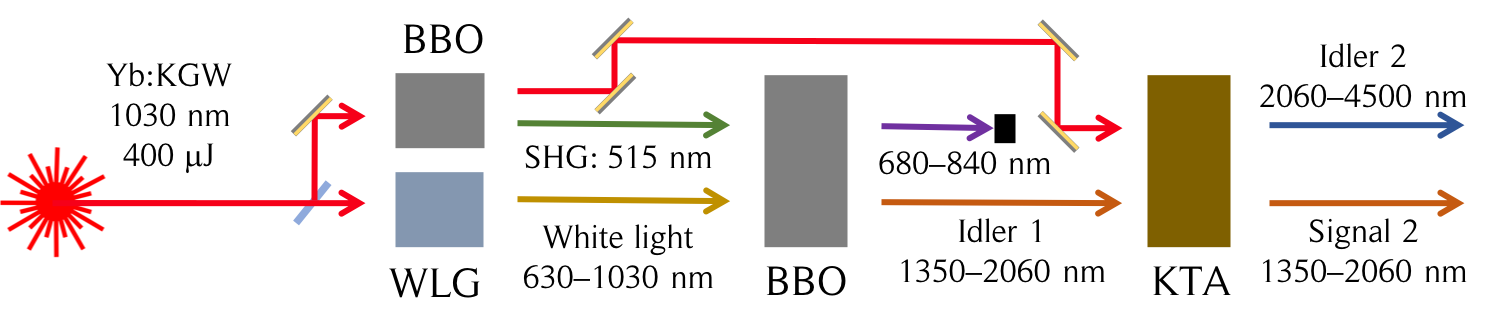
\includegraphics[width=1.0\figwidth]{chapters/Chapter3_Methods2/Graphs/PulsesScheme.png} %The local modes are calculated on the XXX level, and reproduced with permission from ref. XXX. 
	\caption{Schematic of the frequency conversion process to generate ultrafast IR pulses. BBO: barium borate crystal. WLG: white light generation substrate, sapphire. SHG: second harmonic generation. KTA: potassium titanyle arsenate crystal.}
	\label{UltraFastPulses}
\end{figure}






\subsection{Pump-probe optical setup}

As discussed previously in Section \ref{TRVSExp} and expressed in Eq.\ \ref{transientspectra1}, the aim of pump-probe spectroscopy is to measure the time-dependent changes in absorption as a given sample is perturbed by an intense pump pulse. The experimental setup consists of the following elements: pump pulses, probe pulses, a time-modulation translational stage and an IR sensitive detector. A schematic of the setup is shown in Figure~\ref{PumpProbeSetup}.

After setting the laser at the desired frequency, the beam (p-polarized) is directed to a \ce{ZnSe} beam splitter at an incident angle of 45$^o$, which transmits most of the light ($\sim$90\%) to generate the pump beam. The reflected light is directed to a second \ce{ZnSe} beam splitter to form the probe and the reference beam. The pump beam is sent to a computer-controllable translational stage to modulate the pump-to-probe time delay. Using a zero-order $\lambda /$2 plate, the polarization of the pump beam is set to 45$^\circ$ with respect of that polarization of the probe and reference beams. To determine pumped and unpumped transient signals, a chopper blade at a frequency of 500 Hz is placed in the pump optical path. Two wire-grid linear polarizers are used, one for the reference and one for the probe, to filter out undesired perpendicular or elliptical components. 


At this point, pump and probe are focused into the sample at the same spot, while the reference passes through the sample but does not overlap with the other beams. Directly after the sample, a rotating lineal polarizer is used to selectively filter out either the parallel or perpendicular components of the probe and the reference. This enables measurements to be taken in a polarization-resolved manner. After this selective step, the pump beam is blocked, while probe and reference are directed into a grating-based spectrometer that disperses the light onto a 3$\times$32-pixel array MCT (mercury-cadmium-telluride) detector.


\begin{figure}[t!]
	\centering
	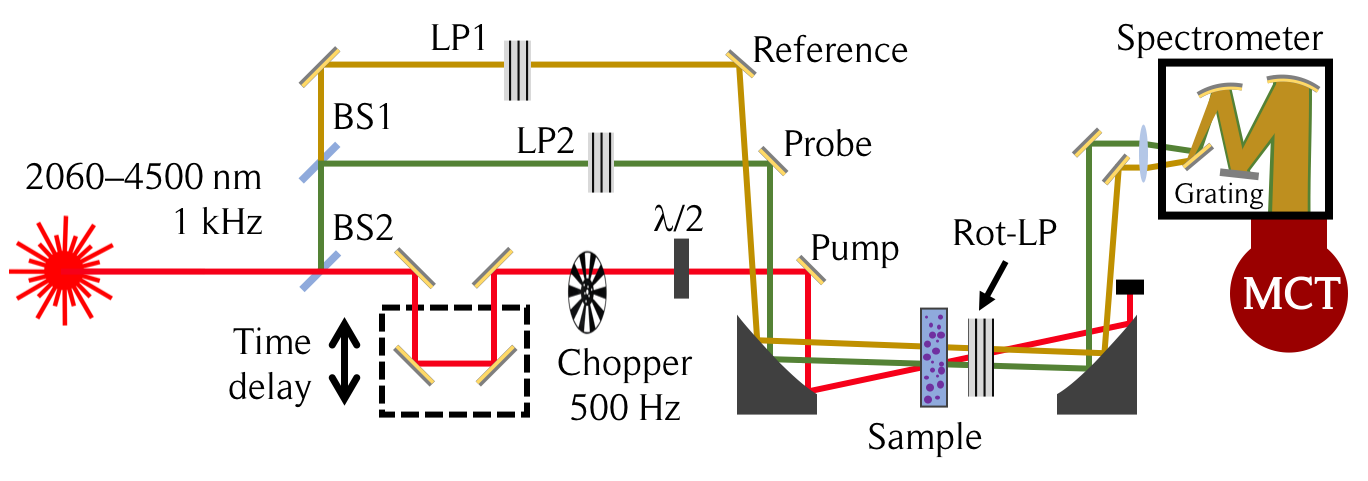
\includegraphics[width=1.0\figwidth]{chapters/Chapter3_Methods2/Graphs/PumpProbeSetup.png} %The local modes are calculated on the XXX level, and reproduced with permission from ref. XXX. 
	\caption{Schematic of the pump-probe optical setup. BS: \ce{ZnSe} beam splitter, LP: wire-grid linear polarizer, $\lambda/2$: zero-order half-wave plate, Rot-LP: rotational wire-grid linear polarizer, MCT: mercury-cadmium-telluride detector.}
	\label{PumpProbeSetup}
\end{figure}



The intensity of the probe is normalized with the intensity of the reference, and the transient absorption change is given by
\begin{eqnarray}
\Delta \alpha (\omega, t ) = - \ln   \underbrace{   \left[  \frac{I_\text{probe} (\omega,t)}{I_\text{ref} (\omega, t)}  \right] }_{\text{pumped}}  +  \ln  \underbrace{ \left[  \frac{I_\text{probe,0} (\omega,t)}{I_\text{ref,0} (\omega, t)}   \right] }_{\text{unpumped}} ,
\end{eqnarray}
which leads to 
\begin{eqnarray}
\nonumber \\
\Delta \alpha (\omega, t ) = - \ln \left[   \frac{I_\text{probe} (\omega,t)}{I_\text{ref} (\omega, t)}        \frac{I_\text{ref,0} (\omega, t)}{I_\text{probe,0} (\omega,t)}         \right] .
\end{eqnarray}

The preceding equation enables us to correct for shot-to-shot intensity fluctuations of the probe. This relation holds valid for both parallel and perpendicular transient absorption.


\section{Data analysis and modeling}\label{TRVSModel}


In this section we describe the the procedures used to extract information from our pump-probe experimental data. The transient signal is characterized by an excited state that decays ultimately into a hot ground state. However, the relaxation mechanism can be quite complicated, since the relaxation process may involve intermediate states. In aqueous solutions, additional excitation may appear due to the inhomogeneities caused by the solutes. One can often distinguish hydration water molecules from those which are far from any ion and behave in a bulk-like manner. In general, ions generate strong local electric field that change the spectra and relaxation rates of vibrations in their immediate vicinity. Therefore, the pump pulse might excite different vibrations at the same time, leading to a complicated spectral response.


We build up the analysis starting with the isotropic signal $\Delta \alpha_{\text{iso}}$, which is insensitive to molecular reorientation. We assume that the relaxation process consists of a linear combination of discrete relaxation steps, where each level is associated to a different spectral component with different population dynamics. As such, we can write
\begin{eqnarray}
\Delta \alpha_{\text{iso}} (\omega, t) = \sum_{i=1}^n \Delta\sigma_i({\omega}) N_i (t),
\label{linearcombiso}
\end{eqnarray}
with $\Delta\sigma_i$ the spectral signature of each constituent component and $N_i$ its corresponding population dynamics. The factor $n$ represents the number of energy levels that the relaxation mechanism possesses.

For the simplest relaxation mechanism, a two-level system, the population dynamics can be represented by the following set of differential equations
\begin{eqnarray}
\frac{d}{d t} \left( \begin{array}{c} N_1 (t) \\ N' (t) \end{array} \right) = \left( \begin{array}{cc} -k_1 & 0 \\ +k_1 & 0 \end{array} \right)  \left( \begin{array}{c} N_1 (t) \\ N' (t) \end{array} \right) \qquad \text{with} \qquad N_i(0) = \left( \begin{array}{c} N_1(0) \\ 0 \end{array} \right),
\label{simplestmodel}
\end{eqnarray}
where $N_1$ and $N'$ refer to the population dynamics of the excited and a final state that is not necessarily the ground state, and the relaxation rate $k_1$ is the reciprocal of the vibrational lifetime $T_1$. Solving these equation leads to the following description
\begin{eqnarray}
\Delta \alpha_{\text{iso}} (\omega, t) = \Delta\sigma_1 (\omega) N_1(0) e^{-k_1 t}  + \Delta\sigma' (\omega) N_1 (0)\left( 1 - e^{-k_1 t} \right),
\end{eqnarray}
where $\Delta \sigma_1 (\omega) = -2 \sigma_{10} (\omega) + \sigma_{21} (\omega)$ is the transient spectral response of the excited state, and $\Delta\sigma' = \sigma'_{10}(\omega) - \sigma_{10} (\omega)$ associated with the final state, as described in Eqs.\ \ref{transientspectra1} and \ref{transientabs2}. This relaxation mechanism is represented in the left side of Figure~\ref{simplestschem}.



\begin{figure}[t!]%* is used because without it the figure does not appear
	\centering	
	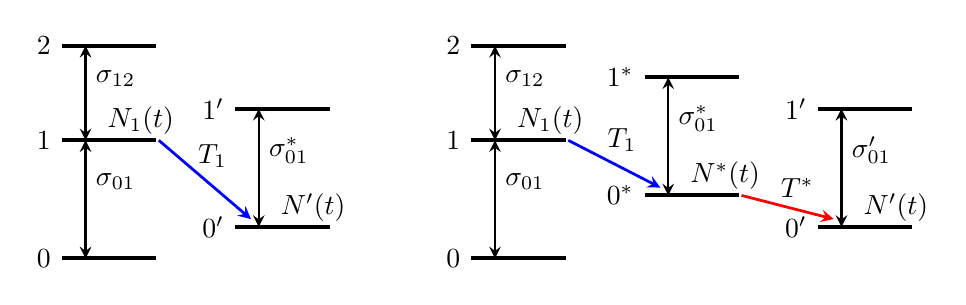
\begin{tikzpicture}[>=stealth,thick]	
	
	%\draw[white,line width=0.05mm](6,4) -- (7.5,4);
	
	\draw[->, line width=0.35mm, blue] (5.03,2.5) -- (6.2,1.9) ;
	\draw[->, line width=0.35mm, red] (7.23,1.8) -- (8.4,1.5);
	
	\draw[<->, line width=0.3mm, black] (4.1,1) -- (4.1,2.5) node[pos=0.65,right] {$\sigma_{01}$};
	\draw[<->, line width=0.3mm, black] (4.1,2.5) -- (4.1,3.7) node[pos=0.65,right] {$\sigma_{12}$};
	
	\draw[<->, line width=0.3mm, black] (6.3,1.8) -- (6.3,3.3) node[pos=0.65,right] {$\sigma_{01}^*$};
	
	\draw[<->, line width=0.3mm, black] (8.5,1.4) -- (8.5,2.9) node[pos=0.65,right] {$\sigma'_{01}$};
	
	\draw[black,line width=0.5mm](3.8,3.7) -- (5,3.7) node[pos=0.0,left] {$\ket{2}$};
	\draw[black,line width=0.5mm](3.8,2.5) -- (5,2.5) node[pos=0.0,left] {$\ket{1}$};
	\draw[black,line width=0.5mm](3.8,1.0) -- (5,1.0) node[pos=0.0,left] {$\ket{0}$};
	
	\draw[black,line width=0.5mm](6,3.3) -- (7.2,3.3) node[pos=0.0,left] {$\ket{1^*}$};
	\draw[black,line width=0.5mm](6,1.8) -- (7.2,1.8) node[pos=0.0,left] {$\ket{0^*}$};
	
	\draw[black,line width=0.5mm](8.2,2.9) -- (9.4,2.9) node[pos=0.0,left] {$\ket{1'}$};
	\draw[black,line width=0.5mm](8.2,1.4) -- (9.4,1.4) node[pos=0.0,left] {$\ket{0'}$};
	
	\node[right,align=left] at (5.4,2.5) {$T_1$};
	\node[right,align=left] at (7.6,1.9) {$T^*$};
	
	
	\node[right,align=left] at (4.25,2.75) {$N_1 (t)$};
	\node[right,align=left] at (6.45,2.05) {$N^* (t)$};
	\node[right,align=left] at (8.65,1.65) {$N' (t)$};
	
	
	
	
	\draw[->, line width=0.35mm, blue] (5.03-5.2,2.5) -- (6.2-5.2,1.5) ;	
	
	
	\draw[black,line width=0.5mm](3.8-5.2,3.7) -- (5-5.2,3.7) node[pos=0.0,left] {$\ket{2}$};
	\draw[black,line width=0.5mm](3.8-5.2,2.5) -- (5-5.2,2.5) node[pos=0.0,left] {$\ket{1}$};
	\draw[black,line width=0.5mm](3.8-5.2,1.0) -- (5-5.2,1.0) node[pos=0.0,left] {$\ket{0}$};
	
	\draw[black,line width=0.5mm](6-5.2,2.9) -- (7.2-5.2,2.9) node[pos=0.0,left] {$\ket{1'}$};
	\draw[black,line width=0.5mm](6-5.2,1.4) -- (7.2-5.2,1.4) node[pos=0.0,left] {$\ket{0'}$};
	
	
	\draw[<->, line width=0.3mm, black] (4.1-5.2,1) -- (4.1-5.2,2.5) node[pos=0.65,right] {$\sigma_{01}$};
	
	\draw[<->, line width=0.3mm, black] (4.1-5.2,2.5) -- (4.1-5.2,3.7) node[pos=0.65,right] {$\sigma_{12}$};
		
	\draw[<->, line width=0.3mm, black] (6.3-5.2,1.4) -- (6.3-5.2,2.9) node[pos=0.65,right] {$\sigma_{01}^*$};
	
	
	\node[right,align=left] at (4.25-5.2,2.75) {$N_1 (t)$};
	\node[right,align=left] at (6.45-5.2,1.65) {$N' (t)$};
%	\node[right,align=left] at (8.65,1.65) {$N' (t)$};
	
	\node[right,align=left] at (5.4-5.2,2.3) {$T_1$};
	
	%\draw[white,line width=0.05mm](1,-0.1) -- (7,-0.1);
	
	\end{tikzpicture}		
	\caption{\textbf{Left:} One-step relaxation mechanism in which the excited oscillators relax directly to a final state (not necessarily the original ground state). \textbf{Right:} Two-step relaxation mechanism in which the excited oscillators decay first to an intermediate state, before attaining the final equilibrium state. The difference between the final state and the original ground state accounts for irreversible changes or heating in the sample due to the intense pump pulse.}
	\label{simplestschem}			
\end{figure}



Unfortunately, the vibrational relaxation process in aqueous systems is never this simple. It has been demonstrated that the vibrational relaxation dynamics of \ce{OD}/\ce{OH} stretch vibrations in isotopically diluted \ce{H2O}/\ce{D2O} is well described by a two-step consecutive model as shown in the right side of Figure~\ref{simplestschem},\!\cite{Rezus2005,Rezus2006} in which the population dynamics are represented with the following differential equations
\begin{eqnarray}
\frac{d}{d t} \left( \begin{array}{c} N_1 (t)\\ N^* (t) \\ N' (t) \end{array} \right) = \left( \begin{array}{ccc} -k_1 & 0 & 0 \\ +k_1 & -k^* & 0 \\ 0 & +k^* & 0 \end{array} \right)  \left( \begin{array}{c} N_1 (t) \\ N^* (t) \\ N' (t) \end{array} \right),
\label{cascademodel}
\end{eqnarray}
where the initial conditions are $N_i (0) = \left(  N_1 (0), 0 , 0   \right)$. In this model, the system relaxes via an intermediate state $\ket{0^*}$ to the hot ground state $\ket{0'}$. 
%In this case, the intermediate state is associated only with a retarded response of the thermal state, with respect to the fast vibrational relaxation. In other words, the coordinates of the hydrogen-bond network take a finite time $T_* = 1/k_*$ to equilibrate with the resulting vibrations from the relaxation process. As such, 
It has been found previously that the intermediate state has the same spectrum as the ground ground state ($\sigma_{01}^* = \sigma_{01}$), meaning that the intermediate state has no associated transient spectrum. In this case, the isotropic transient signal can be model as
\begin{eqnarray}
\Delta \alpha_{\text{iso}} (\omega, t) &=& \Delta\sigma_1 (\omega) N_1(0) e^{-k_1 t} \nonumber \\ &+& \Delta\sigma' (\omega) N_1(0)\left( 1 + \frac{k_1}{k^* - k_1} e^{-k^* t} - \frac{k^*}{k^* - k_1} e^{-k_1 t} \right),
\label{Solutioncascademodel}
\end{eqnarray}
with $\Delta\sigma_1 (\omega) = -2 \sigma_{10} (\omega) + \sigma_{21} (\omega)$ the transient signal of the excited state, and $\Delta\sigma' = \sigma'_{10}(\omega) - \sigma_{10} (\omega)$ the transient signal associated with the hot ground state.


For more complex models, providing a solution to the set of differential equations becomes complicated and tedious for numerical analyses. A easier solution consists of diagonalizing the rate matrix $K$ of the Eqs.\ \ref{simplestmodel} and \ref{cascademodel} written in matrix form as
\begin{eqnarray}
\frac{d}{d t} \vec{N} = K \vec{N}.
\label{differentialK}
\end{eqnarray}

We aim to find a unitary matrix $U$ such that $K U = U \lambda$,
%\begin{eqnarray}
%K U = U \lambda,
%\label{eigenEq2}
%\end{eqnarray}
where $\lambda$ is a diagonal matrix that contains the eigenvalues and $U$ contains the vectors that form the eigenbasis. %In line with this description, the vector $\vec{N}$ corresponds to another as
%\begin{eqnarray}
%\vec{N} (t) = U \vec{M} (t), \qquad \text{where} \qquad \vec{N} (0) = U \vec{M} (0)
%\label{transVector}
%\end{eqnarray}
%holds valid. By using 
%Combining Eqs.\ \ref{differentialK} and \ref{eigenEq2}, we obtain 
As such, the population dynamics are given by
\begin{eqnarray}
\vec{N} (t) = U \exp(\lambda t) U^{-1} \vec{N} (0),
\label{PopuEigen}
\end{eqnarray}
which offers a general solution as a linear combination of exponential decays in terms of the eigenvalues of the rate matrix $K$.



To extract meaningful information from the experimental data $\Delta\alpha_\text{iso}^\text{exp} (\omega,t)$ with standard deviation $\xi (\omega, t)$, we perform least-squares fits to minimize the following weighted $\chi^2$ function
\begin{eqnarray}
\chi^2 = \int \int \left( \frac{\Delta \alpha_\text{iso}^\text{exp} (\omega,t) - \sum_i \Delta\sigma_i(\omega)N_i(t)}{\xi (\omega, t)}\right)^2 dt d\omega,
\label{ChiSquare}
\end{eqnarray}
in which the spectral components $\Delta\sigma_i$ and the decay rate constants \textbf{k} are treated as fit parameters.
%in general, we need a large amount of fitting parameters. However, we aim to find information that allow us to reduce the number of fitting parameters. 


If one knows the relaxation mechanism $K(\text{\textbf{k}})$, the time traces $\vec{N}$ are determined by the \textbf{k} parameters, and we can find the spectral components that minimize the $\chi^2$ function at all times. This method is usually called spectral decomposition. This approach starts out with an estimate for the decay rates \textbf{k}, from which a subsequent minimization process finds the spectral signatures that best fit the experimental data following the expression
\begin{eqnarray}
\frac{d}{d \tilde{\sigma}_i (\omega)} \int \left( \frac{\Delta \alpha_\text{iso}^\text{exp} (\omega,t) - \sum_i \Delta\tilde{\sigma}_i(\omega)N_i(\textbf{k},t)}{\xi (\omega, t)}\right)^2 dt = 0
\label{SpectralDecomp}
\end{eqnarray}
to find the optimal decay rates \textbf{k}. A minimization routine following this approach is shown in Listing \ref{Listing2} using the kinetic model from Eq.\ \ref{cascademodel}.


Analogously, if one knows the spectral components $\Delta\sigma_i$, one can run a minimization process to extract the time traces that best fit the experimental data. This approach is called temporal decomposition, and from
\begin{eqnarray}
\frac{d}{d \tilde{N}_i (t)} \int \left( \frac{\Delta \alpha_\text{iso}^\text{exp} (\omega,t) - \sum_i \Delta\sigma_i(\omega) \tilde{N}_i(t)}{\xi (\omega, t)}\right)^2 d\omega = 0,
\label{TemporalDecomp}
\end{eqnarray}
we obtain the population dynamics. This approach is more convenient for the study of samples in which unconventional processes, such as F\"orster resonance energy transfer,\!\cite{Forster1948} play an important role in the relaxation dynamics. A complete analysis of experimental data that show a F\"orster-like relaxation process is available at \href{https://github.com/RobertoCota/Forster-energy-transfer}{https://github.com/RobertoCota/Forster-energy-transfer}

To extract information on the molecular reorientation dynamics, we use Eqs.\ \ref{isotropicsignal}, \ref{anisotropysignal} and \ref{linearcombiso} to define the following equations
\begin{eqnarray}
\Delta \alpha_\parallel (\omega, t) &=& \sum_{i=i}^n [1 + 2 R_i(t)] N_i (t) \Delta\sigma_i(\omega) = \sum_{i=1}^n N_{i,\parallel} (t) \Delta\sigma_i (\omega) \\
\Delta \alpha_\perp (\omega, t) &=& \sum_{i=i}^n [1 -  R_i(t)] N_i (t) \Delta\sigma_i(\omega) = \sum_{i=1}^n N_{i,\perp} (t) \Delta\sigma_i (\omega),
\end{eqnarray}
in which we associate an anisotropy $R_i (t)$ with each spectral component. To this purpose, we can perform a temporal decomposition minimization on both parallel and perpendicular signals. Having retrieved $N_{i,\parallel} (t)$ and $N_{i,\perp} (t)$, we can calculate the anisotropy of each constituent component as
\begin{eqnarray}
R_i(t) = \frac{N_{i,\parallel} (t) - N_{i,\perp} (t)}{ N_{i,\parallel} (t) + 2 N_{i,\perp} (t)}.
\end{eqnarray}

A global minimization is possible by performing a least-square routine to minimize the following $\chi^2$ function
\begin{eqnarray}
\begin{split}
\chi^2 = \int \int   dt d\omega \left[    \left( \frac{\Delta \alpha_\parallel^\text{exp} (\omega,t) - \sum_i [1 + 2 R_i(t)]N_i(t) \Delta\sigma_i(\omega)}{\xi_\parallel (\omega, t)}\right)^2 \right. \\ \left. +     \left( \frac{\Delta \alpha_\perp^\text{exp} (\omega,t) - \sum_i [1 - R_i(t)]N_i(t) \Delta\sigma_i(\omega)}{\xi_\perp (\omega, t)}\right)^2  \right]  
\label{ChiSquareGlobal}
\end{split}
\end{eqnarray}
where parallel and perpendicular signals are minimized simultaneously. As shown in Chapter \ref{ChapterHydroxide}, this equation can be used to perform spectral decomposition if one defines the relaxation pathway and assign functional forms to each $R_i$ component. An example of this type of analysis is available at \href{https://github.com/RobertoCota/Time-resolved-vibrational-spectroscopy}{https://github.com/RobertoCota/Time-resolved-vibrational-spectroscopy}.


%\newpage
\bigskip
\bigskip

\lstinputlisting[language=Python,caption={Python script for the analysis of isotropic transient absorption in which a two-step consecutive model, represented by Eqs.~\ref{cascademodel} and \ref{Solutioncascademodel}, is used.},label={Listing2}]{chapters/Chapter3_Methods2/Graphs/SpectralDecomposition.py}




% Add an empty page if needed to accomodate properly the chapter image
%%!TEX root = ../thesis.tex

\chapter*{}
%!TEX root = ../thesis.tex


\chapter[Reduced hydrogen-bond cooperativity in ionic solvation shells]{Evidence for reduced hydrogen-bond cooperativity in ionic solvation shells from isotope-dependent dielectric relaxation\myfnt{{\it This chapter is based on:} Roberto Cota, Niklas Ottosson, Huib J. Bakker and Sander Woutersen, \textit{Evidence for reduced hydrogen-bond cooperativity in ionic solvation shells from isotope-dependent dielectric relaxation}, Phys. Rev. Lett. \textbf{2018}, 120, 216001.}}
\label{ChapterPRL}


\vspace{30pt}

We find that the reduction in dielectric response (depolarization) of water caused by solvated ions is different for H$_2$O and D$_2$O. This isotope dependence allows us to reliably determine the kinetic contribution to the depolarization, which is found to be significantly smaller than predicted by existing theory. The discrepancy can be explained from a reduced hydrogen-bond cooperativity in the solvation shell: we obtain quantitative agreement between theory and experiment by reducing the Kirkwood correlation factor of the solvating water from 2.7 (the bulk value) to $\sim$1.6 for NaCl and $\sim$1 (corresponding to completely uncorrelated motion of water molecules) for CsCl.

\newpage

\section{Introduction}


The solvation of ions in water plays a crucial role in numerous physical, chemical and biological processes, ranging from ion transport in fuel cells to the electrostatic screening of DNA. As such, ion hydration is a subject of intense and active experimental and theoretical physical research.\!\cite{LyndenBell1996,Chakraborty2008,Zwolak2009,French2011,Yin2014,Fahrenberger2015}
Dielectric relaxation spectroscopy (DRS, Chapter \ref{ChapterDRS}), is widely used to investigate water and aqueous solutions. With this method crucial information on the structure and dynamics of aqueous solutions can be obtained,\!\cite{Kaatze1993,Buchner1999,Minoguchi2004,Buchner2008,Nakanishi2012,Rahman2012,Perticaroli2013,Ottosson2014c,Balos2015a,Popov2015,Balos2017a} in particular on the effect of ions on the hydrogen-bond network of water.
Ions generate strong local electric fields, orienting the dipole moments of the neighbouring water molecules in solution, and thus causing a reduction in the dielectric response of the water, an effect referred to as depolarization. As has been discussed previously in Section \ref{SectionDepola}, this depolarization is the sum of three contributions: (i)~the dilution of the water solvent,\!\cite{Onsager1936a,Kirkwood1939a,BOTTCHER1973} (ii)~the strongly reduced mobility of water molecules solvating the ions (static depolarization)\!\cite{Barthel1992} and (iii)~the reaction of water molecules to the moving ions (kinetic depolarization): an ion moving in the direction of an externally applied electrical field causes a reorientation of the surrounding water molecules such that their dipoles are directed opposite to the applied field.\!\cite{Hubbard1977a,Hubbard1977,Hubbard1978c,Hubbard1979a,VanderZwan1982,VanderZwan1983a}

To investigate the structure and dynamics of water in electrolyte solutions using DRS, one must separate the different contributions to the depolarization. For the dilution contribution this is trivial, but the static and kinetic depolarization are difficult to separate. A common approach to address this problem is to subtract a theoretical prediction for the kinetic-depolarization contribution from the observed depolarization (corrected for dilution), thus obtaining an estimate for the static depolarization. 
The amplitude of the static depolarization can then be used to estimate the number of water molecules immobilized per solvated cation, the so-called hydration number (the contribution of the anions to the static depolarization is negligible).\!\cite{Impey1983,Guardia1990,Barthel1992,Ohtaki1993,Smith1994,Buchner1999,Wachter2007,Buchner2008,Tielrooij2009,Ottosson2014c} To this purpose, the most commonly used models for kinetic depolarization (originally developed by Onsager and Hubbard,\!\cite{Hubbard1977a,Hubbard1977,Hubbard1978c} and later extended by others\!\cite{VanderZwan1982,VanderZwan1983a,Robinson2002}) integrate the local electromagnetic interactions in the framework of the Navier-Stokes equations of motion for the water. These models provide a closed expression of the kinetic depolarization in terms of the DC conductivity and the Debye relaxation time of the water. As yet, experimental tests of these models for kinetic depolarization are largely lacking. The above-mentioned subtraction procedure sometimes leads to unphysical results, such as negative values for the static depolarization\!\cite{Chen2003} (which would imply negative hydration numbers), which indicates the need for an experimental investigation of kinetic depolarization.



Here, we use the isotope dependence of the depolarization to investigate the kinetic contribution for a series of NaCl and CsCl solutions. We find that the experimentally determined kinetic depolarization is much smaller than the kinetic depolarization that follows from commonly used models. This discrepancy is due to the assumption that the solvating water has the same dielectric response as bulk water, which is incorrect since the ions locally disrupt the hydrogen-bond structure of water.\!\cite{Kay1966,Hertz1974,Hertz1976,Harris1978,Marcus2009,Bakker2009,Lin2009,Jungwirth2014a,Schienbein2017a} 


\section{Experimental}


We record dielectric spectra of NaCl and CsCl solutions in H$_2$O and D$_2$O in the frequency range of 1--50~GHz, which fully covers the main relaxation mode of water at $\sim$$18$~GHz.\!\cite{Ellison1996} The experimental setup used for these experiments is described in Section \ref{ExperimentalDRS}. The complex permittivity of the solutions is recorded for a range of concentrations (0.0--1.0~mol/l). These experiments were carried out at 23$^\circ$C.




The total dielectric permittivity of the solutions is well described by the sum of a Cole-Cole relaxation term for water and an ionic-conductivity term (see Section \ref{DRTheory}):
\begin{eqnarray}
\hat{\epsilon}(\nu) = \epsilon_{\infty} + \frac{\epsilon_{\rm s} - \epsilon_{\infty}}{1 + (i 2 \pi \nu \tau_{\rm D})^{1-\alpha}} - \frac{i \sigma}{2 \pi \nu \epsilon_0},
\label{epsilon}
\end{eqnarray}
where $\epsilon_{\rm s}$ is the static permittivity at low frequencies, $\epsilon_{\infty}$ is the asymptotic permittivity at high frequencies, $\epsilon_0$ is the vacuum permittivity, $\tau_{\rm D}$ the Debye relaxation time, $\alpha$ a parameter characterizing the width of the distribution of relaxation times, $\sigma$ the DC ionic conductivity, and $A_\text{D} = \epsilon_{\rm s} - \epsilon_{\infty}$ the amplitude of the Debye relaxation mode. We determine these parameters by performing a least-squares fit of Eq.\ \ref{epsilon} to the data displayed in Figure~\ref{fig1_Chap4}. The dielectric response at high frequencies is independent of concentration (as has been observed previously\!\cite{Hall1981,Lileev2007,Ottosson2014c}), so in the fit we keep $\epsilon_{\infty}$ fixed to its zero-concentration value. 






\section{Results}


%\begin{figure*}[ht]
\begin{figure}[t!]
	\centering
	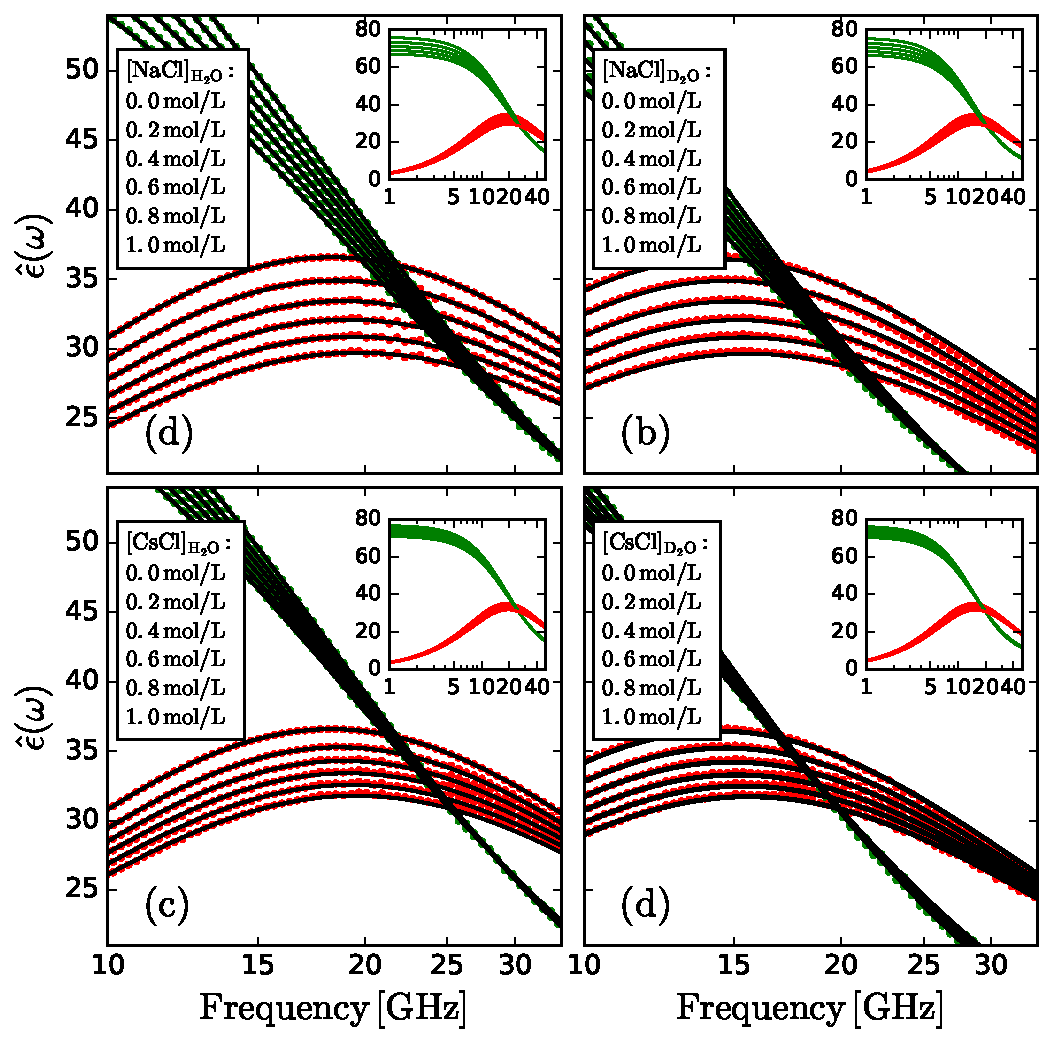
\includegraphics[width=0.9\figwidth]{chapters/Chapter4_PRL/Graphs/RawPermittivity_AllSolutions.pdf}
	\caption{Complex dielectric permittivity spectra of aqueous solutions of NaCl in H$_2$O (a), NaCl in D$_2$O (b), CsCl in H$_2$O (c) and CsCl in D$_2$O ranging from the neat solvent to 1.0 mol/L at 23$^o$C. The red and green dots indicate the data measured by DRS for the dielectric diffusion $\epsilon'(\omega)$ and dielectric losses $\epsilon''(\omega)$, respectively. The solid lines are fits to Eq.~\ref{epsilon}. All data is tabulated in the Appendix.}
	\label{fig1_Chap4}
\end{figure}
%\end{figure*}



Figure~\ref{fig1_Chap4} shows the complex permittivity of the investigated solutions, after subtraction of the ionic-conductivity contribution. Both the addition of NaCl and CsCl leads to a significant reduction of the dielectric response. 
The curves in Figure~\ref{fig1_Chap4} are the result of the least-squares fits, and Figure~\ref{fig2_Chap4}a shows the concentration-dependent conductivity $\sigma$ obtained from the fits. The values in H$_2$O agree well with previous results (see Appendix).\!\cite{Buchner1999,Bianchi1989} The conductivities of all the solutions are well described by the empirical function $\sigma (c) = D c - E c^{3/2}$, which has the same functional form as Kohlrausch's law that applies to dilute solutions. To correct the $A_\text{D}$ obtained from the fit for the trivial dilution effect, we define the concentration-dependent quantity
\begin{eqnarray}
A_\text{D,n}(c) = \frac{c_\text{w}(c)}{c_{\text{w},0}} A_{\text{D},0},
\label{eq4}
\end{eqnarray}
with $A_{\text{D},0}$ and $c_{\text{w},0}$ the amplitude of the Debye relaxation and the molecular concentration of undiluted neat water, and $c_\text{w}(c)$ is the water concentration of the electrolyte solution.
$A_\text{D,n}$ is the (hypothetical) dielectric strength if the only effect of ions in water would be a reduction in water concentration. The dilution-corrected depolarization
\begin{equation}
\Delta A_\text{D} = A_{\text{D,n}} - A_\text{D},
\end{equation}
is the depolarization caused by the interaction of the ions and the water. In the following, the term depolarization will refer to this dilution-corrected quantity $\Delta A_\text{D}$.





Figure~\ref{fig2_Chap4}b shows that the depolarization $\Delta A_\text{D}$ increases with concentration. In addition, there is a small but significant isotope effect: the depolarization is larger for D$_2$O than for H$_2$O solutions. This can be seen more clearly in Figure~\ref{fig3_Chap4}, where we present the isotope-difference $\Delta A_{\rm D}^{\rm H_2O}-\Delta A_{\rm D}^{\rm D_2O}$ as a function of concentration.  Dividing this difference by the value of $\Delta A_{\rm D}$ itself (Fig.~\ref{fig2_Chap4}b), we find that the isotope-effect is $\sim$1.5\% for NaCl and $\sim$3\% for CsCl solution.  The depolarization consists of a static and kinetic contribution:\!\cite{Hubbard1977,Hubbard1977a,Hubbard1979a,VanderZwan1982,VanderZwan1983a,Barthel1992} $\Delta A_{\rm D} = \Delta A_{\text{D,st.}} + \Delta A_{\text{D,kin.}}$ The dipole moments of H$_2$O and D$_2$O differ by only 0.06\%,\!\cite{Clough1973} which is negligible compared to the observed isotope effect, and to the uncertainty in our data. Hence, the static contributions to the depolarization can be assumed equal for H$_2$O and D$_2$O, so that 
\begin{equation}
\Delta A_{\rm D}^{\rm H_2O}-\Delta A_{\rm D}^{\rm D_2O} = \Delta A_{\rm D,kin.}^{\rm H_2O}-\Delta A_{\rm D,kin.}^{\rm D_2O}
\label{Skin} 
\end{equation}

The preceding result enables us to determine the kinetic depolarization independently from the static depolarization. In particular, we can directly compare the experimentally observed $\Delta A_{\rm D,kin.}^{\rm H_2O}-\Delta A_{\rm D,kin.}^{\rm D_2O}$ to theoretical predictions.  




%\begin{figure*}[ht]
\begin{figure}[t!]
	\centering
	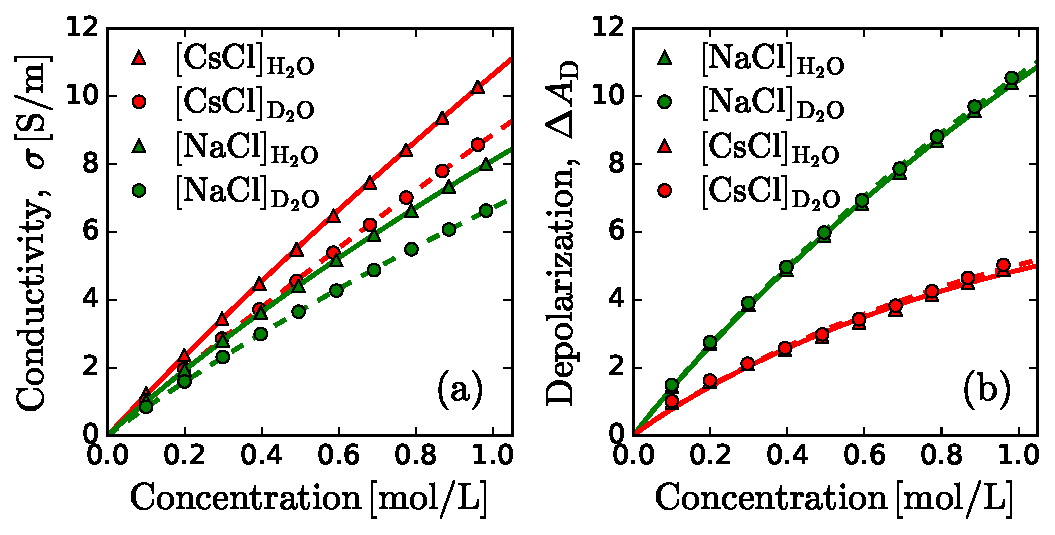
\includegraphics[width=0.85\figwidth]{chapters/Chapter4_PRL/Graphs/Conductivity_and_Depolarization.pdf}
	\caption{(a)~Conductivity $\sigma$ as a function of the salt concentration for four salt solutions. (b)~Depolarization as a function of concentration for the same solutions as in the left panel. The triangles and circles represent ions dissolved  in H$_2$O and D$_2$O, respectively; red and green refer to solutions with Na$^+$ and Cs$^+$ ions, respectively.}
	\label{fig2_Chap4}
\end{figure}
%\end{figure*}

\section{Determining the reduced cooperativity of water near ions}




The most commonly used model for kinetic depolarization is the continuum model derived by Hubbard and Onsager\!\cite{Hubbard1977,Hubbard1979a} (see Section \ref{SectionDepola}). In this model, the response of the water surrounding the moving ions is described as a continuum exhibiting the same Debye-relaxation behaviour as bulk neat water. Provided that the viscous frictional forces are much larger than 
the dielectric drag, the predicted kinetic depolarization is then given by
\begin{eqnarray}
\Delta A_{\text{D,kin.}}^{\rm HO} = p \sigma(c)  \left( \frac{ \tau_{\rm D} }{  \epsilon_0} \cdot \frac{\epsilon_s -\epsilon_{\infty}}{\epsilon_s }   \right),
\label{HOeq}
\end{eqnarray}
where $\sigma(c)$ is the concentration-dependent specific conductivity, $\tau_{\rm D}$ the Debye-relaxation time, and $p$ a factor which characterizes the tangential contact forces between the water molecules and ion surface, the limiting cases being perfect slip (no tangential force, $p = 2/3$), and perfect stick (infinite tangential force, $p=1$). This equation has no explicit dependence on the size of the ions. 
Since we measure all the parameters entering Eq.\ \ref{HOeq} for both H$_2$O and D$_2$O, we can directly test the validity of the Hubbard-Onsager model for the kinetic depolarization using Eq.~\ref{Skin}. The red lines in Figure~\ref{fig3_Chap4} are the theoretical predictions  for perfect slip (solid lines) and perfect stick (dashed lines). Clearly, the Hubbard-Onsager model predicts a much larger H$_2$O/D$_2$O difference in kinetic depolarization than is observed experimentally.

In a later, more rigorous theory for the kinetic depolarization, Hubbard, Colonomos and Wolynes describe the system as ionic spheres immersed in a solution of rotating dipoles, which are again assumed to exhibit Debye relaxation identical to that of bulk water. In this model the finite size of the solvent molecules is taken into account (as opposed to the earlier continuum model). They obtained an expression for the depolarization in which the radius of the ion occurs explicitly:\!\cite{Hubbard1979a} 
\begin{eqnarray}
\Delta A_{\text{D,kin.}}^{\rm HCW} = \frac{p \sigma(c) \tau_{\rm D}}{ \epsilon_0} \left[ \frac{N R_i}{e} \left\langle \frac{ \vec{\mu} \cdot \hat{r}}{r^2} \right\rangle \right], 
\label{HCWeq}
\end{eqnarray}
where $N$ is the number of water dipoles per volume unit, $R_i$ the ionic radius, $\mu$ the water molecule dipole moment, $r$ the distance between the water molecule and the ion and $e$ the ionic charge. In Ref.~\citenum{Hubbard1979a} the authors numerically evaluated the number in square brackets in Eq.~\ref{HCWeq}, in particular for Na$^+$, Cs$^+$ and Cl$^-$. 
The $\Delta A_{\text{D,kin.}}^{\text{H}_2\text{O}} - \Delta A_{\text{D,kin.}}^{\text{D}_2\text{O}}$ predicted by this theory is shown as the green lines in Figure~\ref{fig3_Chap4}, again for both limiting values of $p$. Again, the theory predicts a much larger difference in kinetic depolarization than is observed experimentally.


%\begin{figure*}[ht]
\begin{figure}[t!]
	\centering
	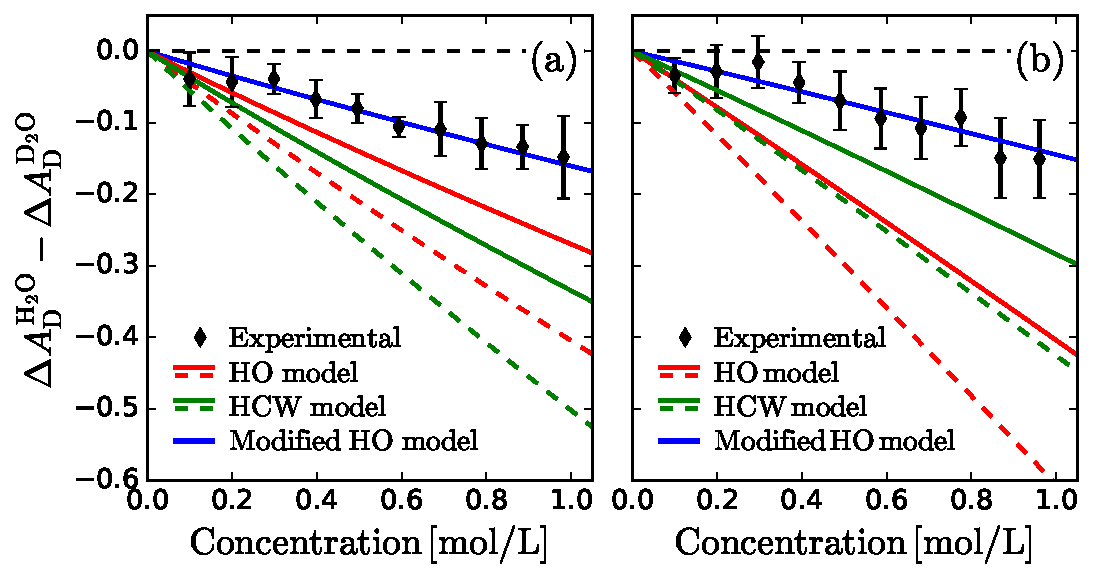
\includegraphics[width=0.85\figwidth]{chapters/Chapter4_PRL/Graphs/Onsager_Sodium_Caesium_EffectiveKirkwood_with_Fitting.pdf}
	\caption{(a)~Difference between the depolarization of NaCl in H$_2$O and the depolarization of NaCl in D$_2$O as a function of concentration. (b)~Difference between the depolarization of CsCl in H$_2$O and the depolarization of CsCl in D$_2$O as a function of concentration. The experimental results are represented by the diamonds. The solid lines represent calculations of the depolarization difference with different models for the kinetic depolarization using $p=2/3$ (solid lines) and $p=1$ (dashed lines). The solid blue line represents a fit to the data with the modified Hubbard-Onsager model of Eq.~\ref{eq:HOM}.}
	\label{fig3_Chap4}
\end{figure}
%\end{figure*}


The discrepancy between the theoretically predicted and experimentally observed kinetic depolarization can be explained if the water surrounding the ions exhibits a smaller dielectric response than bulk water. In neat water, the highly organized hydrogen-bond structure leads to highly cooperative reorientational motion of water molecules. As a consequence, the theory for the dielectric response of a liquid consisting of randomly moving dipoles (originally derived by Onsager\!\cite{Onsager1936a}) predicts a dielectric constant that is much smaller than observed. This is phenomenologically corrected in the Kirkwood-Fr\"ohlich equation:
\begin{equation}
\frac{(\epsilon_{\rm s}-\epsilon_\infty)(2\epsilon_{\rm s}+\epsilon_\infty)}
{\epsilon_{\rm s}(\epsilon_\infty+2)^2}=\frac{\rho \mu^2 g_\text{K}}{9 \epsilon_0 k_{\rm B}T} \qquad
\Rightarrow \qquad
\epsilon_{\rm s} \approx \frac{\rho \mu^2 g_\text{K}}{18 \epsilon_0 k_{\rm B} T}{(\epsilon_\infty + 2)^2},
\label{kirkwoodfroelich}
\end{equation}
where $\rho$ is the density of water molecules, $k_{\rm B}$ Boltzmann's constant, $\mu$ the molecular dipole moment, and $g_\text{K}$ the Kirkwood correlation factor  (see Section~\ref{KirkFrohSection}). The limit $g_\text{K}=1$ corresponds to completely uncorrelated motion of the molecules, and $g_\text{K}>1$ to correlated motion. For bulk liquid water, the experimentally determined value is $g_\text{K,bulk}= 2.7$. As can be seen in Eq.~\ref{kirkwoodfroelich}, the Kirkwood factor effectively scales up the dielectric response with respect to its theoretical value in the case of completely uncorrelated orientational motion.

The Hubbard-Onsager expression for the kinetic depolarization assumes that the dielectric response of water surrounding ions is the same as that of bulk water, i.e.\ that it has a Kirkwood factor of 2.7. However, ions tend to disrupt the hydrogen-bond structure of liquid water, and thus the reorientation of the water molecules surrounding the ions will be less correlated than that of the molecules in bulk water. To account for this effect, we modify the Hubbard-Onsager expression as follows:
\begin{equation}
%\Delta S_{\rm kin.}^{\rm eff.} = \left(\frac{g_{\rm ion}}{g_{\rm bulk}}\right) \Delta S_{\rm kin.}^{\rm HO}
\Delta A_{\text{D,kin.}}^{\rm HO,mod.} = \frac{p \sigma(c) \tau_{\rm D} }{ \epsilon_0 }\frac{g_\text{K,ion}}{g_\text{K,bulk}} \left[ \frac{\epsilon_s -\epsilon_{\infty}}{\epsilon_s } \right],
\label{eq:HOM}
\end{equation}
%\begin{figure*}[ht]
\begin{figure}[t!]
	\centering
	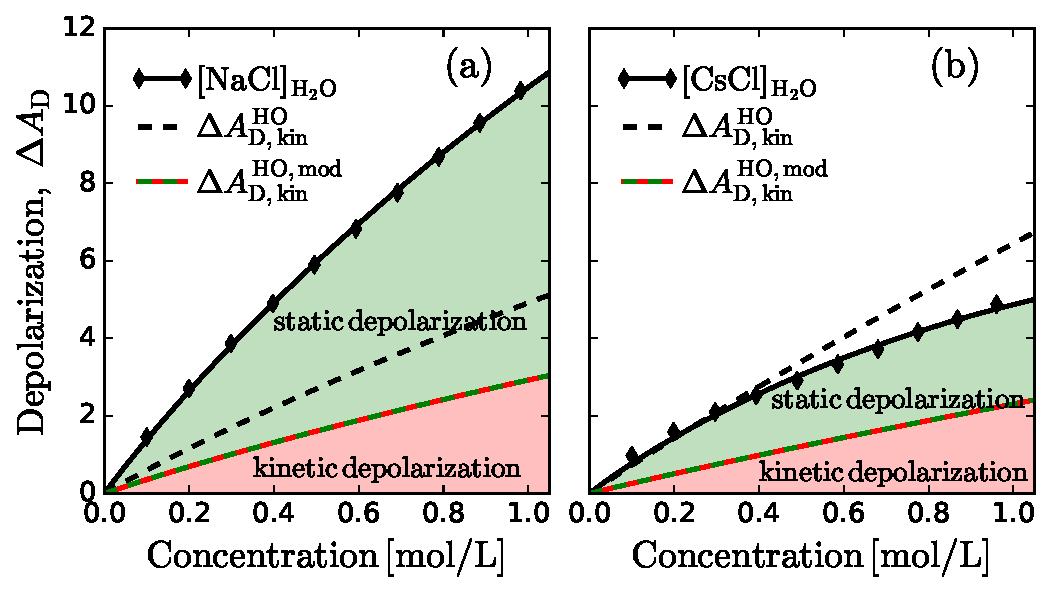
\includegraphics[width=0.85\figwidth]{chapters/Chapter4_PRL/Graphs/DepolarizationSeparation2.pdf}
	\caption{Experimentally observed total depolarization (corrected for dilution) of NaCl (a) and CsCl (b) in H$_2$O, and its decomposition into the static and the kinetic depolarization using the modified Onsager-Hubbard model~(Eq.\ \ref{eq:HOM}). The dashed black curve shows the kinetic depolarization predicted by the conventional Hubbard-Onsager equation. In the case of CsCl the conventional Hubbard-Onsager equation predicts a kinetic depolarization that is larger than the observed total depolarization, which would imply a negative static depolarization, and thus a negative hydration number.}
	\label{fig:HOM}
\end{figure}
%\end{figure*}
where we have introduced an effective Kirkwood factor $g_\text{K,ion}$ for the water surrounding the ions. The value of $g_\text{K,ion}$ can be determined by fitting the above equation to the experimental data (and using the known value of $g_\text{K,bulk}$), see the blue lines in Figure~\ref{fig3_Chap4}. We find $g_\text{K,ion}$ values of 1.6$\pm$0.1 and 1.0$\pm$0.2 for Na$^+$ and Cs$^+$, respectively. The smaller value for Cs$^+$ compared to Na$^+$ is due to a stronger propensity to break up the hydrogen-bond structure of water. This result is in line with previous investigations of the relation between water structure and ionic mobility,\!\cite{Kay1966,Hertz1974,Hertz1976,Harris1978} which showed faster ionic diffusion in less structured hydrogen-bond environments. At high concentrations, the Hubbard-Onsager theory will also overestimate the amplitude of the kinetic depolarization because this theory does not include the Debye screening of the potential of the moving charge due to the dynamic repositioning of the other ions in the medium. We will not consider this effect here, but we hope that our experiments will stimulate further experimental and theoretical work in this direction.






Using the modified Hubbard-Onsager equation, we can now decompose the observed (dilution-corrected) depolarization into its static and kinetic contributions in a well-defined manner. The result is shown in Figure~\ref{fig:HOM}, which also displays the kinetic depolarization predicted by the conventional Hubbard-Onsager equation (Eq.~\ref{HOeq}). Note that by subtracting the latter from the total depolarization one obtains a negative static depolarization for CsCl, which is not physically meaningful. Using the modified Hubbard-Onsager equation we obtain a positive (physically meaningful) static depolarization.




\section{Discussion and conclusion}


From the amplitude of the static depolarization we can directly estimate the number of water molecules that are rotationally immobilized per ion, i.e.\ the hydration number.\!\cite{Barthel1992} We obtain hydration numbers of 8.1$\pm$0.9 for Na$^+$ and 3.1$\pm$1.0 for Cs$^+$. These numbers agree well with previous estimates obtained using more indirect measurements.\!\cite{Richens1997} Both for Na$^+$ and Cs$^+$ the hydration number (the number of rotationally immobilized water molecules) is different from the coordination number (the number of water molecules that in the first solvation shell: 6 and 8 for Na$^+$ and Cs$^+$ respectively).\!\cite{Ohtaki1993,White2000,Varma2006,Mason2006,Rowley2012} This difference is a general phenomenon\!\cite{Barthel1992} which illustrates the importance of experimentally determining the hydration number.

To conclude, the observed isotope effect in the depolarization of ionic solutions indicates that water molecules surrounding ions reorient in a much less cooperative manner than in neat bulk water, with Kirkwood factors close to unity. Based on our observations we propose a modified Hubbard-Onsager equation that takes the locally reduced Kirkwoord factor into account, and that makes it possible to analyze the depolarization of ionic solutions in an unambiguous manner.  This modified Hubbard-Onsager equation provides meaningful hydration numbers, which the conventional Hubbard-Onsager equation fails to do (in some cases even leading to unphysical results) because this expression overestimates the collective nature of water reorientation near ions. Our results thus provide new insights into the effect of ions on water cooperativity. The approach presented here enables a reliable determination of hydration numbers, which is of broad physical relevance, since hydration numbers are widely used to quantify the physical and chemical properties of aqueous solutions.




% Add an empty page if needed to accomodate properly the chapter image
%%!TEX root = ../thesis.tex

\chapter*{}
%\include{chapters/Chapter5...}

% Add an empty page if needed to accomodate properly the chapter image
%%!TEX root = ../thesis.tex

\chapter*{}
%\include{chapters/Chapter6...}

% Add an empty page if needed to accomodate properly the chapter image
%%!TEX root = ../thesis.tex

\chapter*{}
%\include{chapters/Chapter7...}

\end{spacing}
%%%%%%%%%%%%%%%%%%%%%%%%%%%%%%%%%%%%%%%%%%%%%%


%%%%%%%%%%%%%%%%%%%%%%%%%%%%%%%%%%%%%%%%%%%%%%
\begin{spacing}{\dcompressedspacing}
	\small
			
	\renewcommand\refname{} 
	\addcontentsline{toc}{chapter}{References}%{Epilogue references}
	\renewcommand\bibname{References}
	\bibliographystyle{achemso}
	
	% Import bibtex files
	\bibliography{bibliography/library,bibliography/CP2K}
	

\end{spacing}
\normalsize
%\lhead[\fancyplain{}]{{}}
%\rhead[\fancyplain{}]{{}}


%%%%%%%   ADDITIONAL TO THE CHAPTERS   %%%%%%%%%%
\begin{spacing}{\dcompressedspacing}
	

%!TEX root = ../thesis.tex

\chapter*{Appendix}
\markboth{Appendix}{Appendix}
\vspace*{20pt}

% Add label in the list of contents
\addcontentsline{toc}{chapter}{Appendix}

\begin{center}
	\textcolor{SchoolColor}{\Titulosize\bfseries Dielectric properties of electrolyte solutions} \normalsize \\
	\vspace*{20pt}
\end{center}

\setcounter{table}{0}
\renewcommand\thetable{A.\arabic{table}}

Complex dielectric spectra were measured for a series of metal-alkali chloride (MCl with M $=$ Na$^+$, K$^+$, Rb$^+$ and Cs$^+$) solutions both in H$_2$O and D$_2$O. For the study of protons (\ce{H+}) and hydroxide (\ce{OH-}) ion, we recorded complex dielectric spectra for the following solutions: \ce{HCl} and \ce{NaOH} dissolved in \ce{H2O} and \ce{DCl} and \ce{NaOD} dissolved in \ce{D2O}. Calibration of the setup was made prior measurements using air (open circuit), deionized water (5.5 $\mu$S/m) at 23$^\circ$C and silver paint (short circuit). The dielectric properties of pure H$_2$O were extracted from previously reported values by Buchner and co-workers.\!\cite{Buchner1999}

%Complex dielectric spectra were measured for a series of metal-alkali chloride (MCl with M $=$ Na$^+$, K$^+$, Rb$^+$ and Cs$^+$) solutions both in H$_2$O and D$_2$O. For the study of protons (\ce{H+}) and hydroxide (\ce{OH-}) ion, we recorded complex dielectric spectra for the following solutions: \ce{HCl} and \ce{NaOH} dissolved in \ce{H2O} and \ce{DCl} and \ce{NaOD} dissolved in \ce{D2O}. Calibration of the setup was made prior measurements using air (open circuit), deionized water (5.5 $\mu$S/m) at 23$^\circ$C and silver paint (short circuit). The dielectric properties of pure H$_2$O were extracted from previously reported values by Buchner and co-workers.\!\cite{Buchner1999}

To systematically study solvation properties, we perform concentration-dependent measurements in steps of 0.1 molal (or 0.1 molar for the study of protons and hydroxide ions), and determine the amplitude of the Debye dipole relaxation, $A_\text{D}$. The densities of all the samples were measured to estimate the solute molarity, $c$, and to account for the reduction of $A_\text{D}$ due to dilution of the solvent, referred to as $A_\text{D,n}$.


As discussed in previous chapters, the dielectric permittivity of aqueous electrolytes is well described using the Cole--Cole relaxation model, with an additional contribution assigned to the translational motion of ions through the solution, i.e. ionic conductivity. The total permittivity is determined by performing a least-square fit of the following equation: 
\begin{eqnarray}
\hat{\epsilon}(\nu) = \epsilon_{\infty} + \frac{\epsilon_{\rm s} - \epsilon_{\infty}}{1 + (i 2 \pi \nu \tau_{\rm D})^{1-\alpha}} - \frac{i \sigma}{2 \pi \nu \epsilon_0}, \nonumber
\label{Permittivity}
\end{eqnarray}
with $A_\text{D} (c) = \epsilon_s (c) - \epsilon_\infty$, $\tau_D$ the average dipole relaxation time, $\alpha$ accounts for the spectral broadening due to inhomogeneities upon adding ions to the solvent, $\sigma$ the DC ionic conductivity and $\epsilon_0$ the vacuum permittivity. Based on previous results,\!\cite{Lileev2007} the dielectric response of the solvent in the high frequency range, $\epsilon_\infty$, is independent of ion concentration. Therefore, to reduce the number of fitting parameters and to achieve better agreement in our values, we fixed $\epsilon_\infty$ to the value for pure solvent. However, since experimental values for the dielectric properties of D$_2$O are largely lacking, we first performed measurements of pure D$_2$O at 23$^\circ$C, and determined its dielectric properties using equation (\ref{Permittivity}) with $\alpha = 0$ and $\sigma = 0$, leading to $\epsilon_\infty = 5.803$, $A_\text{D} (0) = 72.783$ and $\tau_\text{D} (0) = 11.07$ ps.

Apart from the dilution of the solvent, dissolved ions also exert a strong influence on the orientational motion of the surrounding water molecules, an effect conventionally referred as depolarization. To unambiguously account for this effect, we defined $\Delta A_\text{D} (c) = A_\text{D,n} (c) - A_\text{D} (c)$. Tables \ref{my-label}--\ref{my-label12} summarize all the experimental values extracted for dielectric properties of the studied solutions.




\begin{table}[!ht]
	\centering
	\caption{Molality, m [mol/kg], density, $\rho$, ionic concentration, $c$ [mol/dm$^3$], reduced dielectric response due to dilution of the solvent, $A_\text{D,n}$, depolarization, $\Delta A_\text{D}$, dielectric relaxation parameters $\tau_\text{D}$, $\alpha$ and specific conductivity, $\sigma$, of NaCl in H$_2$O at 23$^\circ$C.}
	\label{my-label}
	\begin{tabular}{cccccccc}
		\hline
		m & $\rho$ [g/dm$^3$] & $c$ & $A_\text{D,n}$ & $\Delta A_\text{D}$ & $\tau_\text{D}$ [ps] & $\alpha$ & $\sigma$ [S/m] \\
		\hline
		0.1 & 1000.65   & 0.0996 & 73.043   & 1.452(33)      & 8.598    & 0.0006 & 1.025(4)  \\
		0.2 & 1004.75   & 0.1993 & 72.916   & 2.706(15)      & 8.538    & 0.0031 & 1.938(7)  \\
		0.3 & 1008.77   & 0.2984 & 72.786   & 3.870(20)      & 8.455    & 0.0050 & 2.806(9)  \\
		0.4 & 1012.70   & 0.3973 & 72.650   & 4.901(23)      & 8.398    & 0.0075 & 3.623(8)  \\
		0.5 & 1016.67   & 0.4954 & 72.521   & 5.904(20)      & 8.342    & 0.0098 & 4.410(5)  \\
		0.6 & 1020.57   & 0.5933 & 72.387   & 6.827(7)       & 8.299    & 0.0121 & 5.175(6)  \\
		0.7 & 1024.50   & 0.6913 & 72.255   & 7.761(33)      & 8.240    & 0.0142 & 5.914(5)  \\
		0.8 & 1028.40   & 0.7886 & 72.124   & 8.684(18)      & 8.190    & 0.0164 & 6.639(10) \\
		0.9 & 1032.25   & 0.8854 & 71.991   & 9.565(17)      & 8.137    & 0.0186 & 7.338(6)  \\
		1.0 & 1036.00   & 0.9819 & 71.853   & 10.396(52)     & 8.099    & 0.0212 & 8.003(28) \\
		\hline
	\end{tabular}
\end{table}


\begin{table}[!ht]
	\centering
	\caption{Molality, m [mol/kg], density, $\rho$, ionic concentration, $c$ [mol/dm$^3$], reduced dielectric response due to dilution of the solvent, $A_\text{D,n}$, depolarization, $\Delta A_\text{D}$, dielectric relaxation parameters $\tau_\text{D}$, $\alpha$ and specific conductivity, $\sigma$, of NaCl in D$_2$O at 23$^\circ$C.}
	\label{my-label2}
	\begin{tabular}{cccccccc}
		\hline
		m & $\rho$ [g/dm$^3$] & $c$   & $A_\text{D,n}$ & $\Delta A_\text{D}$ & $\tau_\text{D}$ [ps] & $\alpha$ & $\sigma$ [S/m] \\
		\hline
		0.1 & 1108.00 & 0.0997 & 72.756 & 1.491(17)  & 10.931 & 0.0019 & 0.845(3)  \\
		0.2 & 1111.92 & 0.1992 & 72.631 & 2.749(32)  & 10.830  & 0.0006 & 1.592(6)  \\
		0.3 & 1115.93 & 0.2984 & 72.513 & 3.909(9)   & 10.732 & 0.0033 & 2.314(7)  \\
		0.4 & 1119.82 & 0.3971 & 72.389 & 4.969(13)  & 10.651 & 0.0055 & 2.991(6)  \\
		0.5 & 1123.63 & 0.4956 & 72.260 & 5.984(5)   & 10.575 & 0.0080 & 3.650(9) \\
		0.6 & 1127.35 & 0.5935 & 72.129 & 6.933(12)  & 10.500 & 0.0103 & 4.273(9) \\
		0.7 & 1131.10 & 0.6913 & 71.999 & 7.870(18)  & 10.432 & 0.0127 & 4.878(3)  \\
		0.8 & 1134.95 & 0.7886 & 71.877 & 8.813(31)  & 10.336 & 0.0148 & 5.491(17) \\
		0.9 & 1138.57 & 0.8860 & 71.741 & 9.699(26)  & 10.258 & 0.0169 & 6.073(17) \\
		1.0 & 1142.20 & 0.9825 & 71.608 & 10.545(26) & 10.191 & 0.0190 & 6.631(16) \\
		\hline
	\end{tabular}
\end{table}





%!TEX root = ../thesis.tex

\chapter*{Summary}
\markboth{Summary}{Summary}

% Add label in the list of contents
\addcontentsline{toc}{chapter}{Summary}

\begin{center}
	\textcolor{SchoolColor}{\Titulosize\bfseries Unraveling the elusive solvation structure of aqueous ions using advanced spectroscopic techniques} \normalsize \\
	\vspace*{9pt}
\end{center}


In this thesis, we investigate the solvation of ions in water using state-of-the-art spectroscopic techniques: GHz dielectric relaxation spectroscopy (DRS) and femtosecond time-resolved vibrational spectroscopy (TRVS), which are introduced in \textbf{Chapters 2} and \textbf{3}. In \textbf{Chapters 4}, \textbf{5}, and \textbf{6}, we demonstrate how DRS can be used to investigate solvation properties and the structure of water around ions. In \textbf{Chapters 7}, \textbf{8} and \textbf{9}, we apply TRVS to observe how the negatively charged oxygen atom of hydroxide and phenolate ions, which act as strong hydrogen-bond acceptors, affects the structural dynamics of the hydrogen-bond network of water.


In the experiments presented in \textbf{Chapter 4}, we study the extent to which the cooperative dynamics of water are affected by the presence of ions. Isotope-dependent measurements enable us to observe the dielectric response of water molecules surrounding ions. Our results indicate that these water molecules reorient in a much less cooperative manner than bulk water, as a consequence of the local disruption of the hydrogen-bond network by the ions. Our observations allow us to test for the first time and to empirically modify the Hubbard-Onsager model that quantifies the ion-induced dielectric deficiency of water. In contrast to the original model, the modified Hubbard-Onsager equation takes the disruption of the hydrogen-bond network by the ions into account, making it possible to determine hydration numbers in an unambiguous manner. These numbers are of paramount importance since they characterize the chemical and physical properties of aqueous solutions. 


In \textbf{Chapter 5}, the isotope effect is again used to determine hydration numbers of alkali-metal ions. Based on our observations, \ce{Na+} forms solvation shells of $\sim$7 water molecules, a hydration number slightly larger than the packing capacity of water in the first solvation shell. Upon increasing the size of the ion, the hydration number reduces to 4, 3 and 3 for \ce{K+}, \ce{Rb+} and \ce{Cs+}, respectively. In these three cases, the hydration number is smaller than the packing capacity, meaning that the first solvation shell is weakly hydrated. Our results are in line with the Hofmeister series which establishes the relative hydration ability of water depending on electrostatic ion--water interactions. 


Protons (\ce{H+}) and hydroxide ions (\ce{OH-}) are cases of special interest since they have the ability to form hydration complexes in which the excess charge is delocalized. In \textbf{Chapter~6}, we measure the isotope-dependent dielectric response to study the solvation of \ce{H+} and \ce{OH-} ions. From its hydration number, \ce{H+} is found to mostly exist in water as an Eigen H$_9$O$_4^+$ complex. From the study of the kinetic effects, we estimate the number of water molecules that are involved in the \ce{H+} and \ce{OH-} charge diffusion. This number is at least three times higher for \ce{H+} than for \ce{OH-}, meaning that the proton transfer mechanism is significantly different in acidic and alkaline solutions. 


In \textbf{Chapter 7}, we explore the extent to which \ce{OH-} ions affect the reorientation dynamics of water molecules. We examine whether \ce{OH-} can have an influence on the molecular dynamics of the solvent (water molecules beyond the first solvation shell). For solutions with \ce{OH-} concentration up to 4 molar, the reorientation dynamics of water are slightly slowed down. At higher \ce{OH-} concentrations, the remaining bulk-like solvent is cooperatively locked between neighboring \ce{OH-} ions due to a crowding effect. In this regime, the solution can be regarded as a semi-rigid hydrogen-bond network.


In \textbf{Chapter 8}, we continue our study of the structural properties of \ce{OH-} ions, but with a focus on the role that they could play in equilibrating vibrational excess energy of surrounding water molecules. We observe that hydroxide ions accelerate the relaxation of OD-stretch excitations of nearby HDO molecules. This effect is well-described through resonance energy transfer from HDO to \ce{OH-} with a F\"orster radius of 3~\AA, a value that matches the intermolecular distance in liquid water. Hence, \ce{OH-} ions act as a sink for excess vibrational energy of neighbouring excited water molecules. Our results suggest that \ce{OH-} ions may also participate in equilibrating excess energy in chemical reactions in alkaline environments.


Finally, in \textbf{Chapter 9}, we study how phenolate ions affect the reorientation dynamics of surrounding water molecules. Our results show that phenolate slows down the dynamics of the surrounding water molecules, an effect that extends even beyond the first solvation shell. This effect is due to the propensity of the negatively charged oxygen to form strong hydrogen bonds, which ``lock'' the hydrogen-bond structure.


The results presented in this thesis provide new information on the solvation properties of several commonly occupied ions. We hope that this thesis will inspire further experimental and theoretical studies, and may help to improve our understanding of the solvation structure and dynamics of ions in water.





%!TEX root = ../thesis.tex

\chapter*{Samenvatting}
\markboth{Samenvatting}{Samenvatting}

% Add label in the list of contents
\addcontentsline{toc}{chapter}{Samenvatting}


\begin{center}
	\textcolor{SchoolColor}{\Titulosize\bfseries Het ontrafelen van de raadselachtige structuur van water rondom ionen met behulp van geavanceerde spectroscopische technieken} \normalsize \\
	\vspace*{9pt}
\end{center}


In dit proefschrift onderzoeken we hoe ionen oplossen in water, waarbij we gebruik maken van \textit{state-of-the-art} spectroscopische technieken: gigahertz di\"{e}lektrische relaxatiespectroscopie (DRS) en femtoseconde tijdsopgeloste vibrationele spectroscopie (TRVS). Deze technieken worden ge\"{i}ntroduceerd in \textbf{Hoofdstukken 2} en \textbf{3}. In \textbf {Hoofdstukken 4}, \textbf{5} en \textbf{6} laten we zien hoe DRS kan worden gebruikt om de eigenschappen van water rond ionen te onderzoeken. In \textbf{Hoofdstukken 7}, \textbf{8} en \textbf{9} passen we TRVS toe om de invloed van het negatief geladen zuurstofatoom in hydroxide- en fenolaat-ionen---beide sterke waterstofbrug-acceptoren---op de structuur en dynamica van het waterstofbrug-netwerk van water te bekijken.


In \textbf{Hoofdstuk 4} onderzoeken we de mate waarin de co\"{o}peratieve dynamica van water wordt be\"{i}nvloed door de aanwezigheid van ionen. Door isotoop-afhankelijke metingen uit te voeren kunnen we de di\"{e}lektrische respons van watermoleculen rondom ionen waarnemen. Uit onze resultaten blijkt dat deze watermoleculen op een veel minder co\"{o}peratieve manier reori\"{e}nteren dan bulkwater, als gevolg van de lokale verstoring van het waterstofbrug-netwerk door de ionen. Onze waarnemingen stellen ons in staat om het Hubbard-Onsager model voor het eerst experimenteel te testen. Dit model beschrijft de door ionen veroorzaakte vermindering van de di\"{e}lektrische respons van water. Uit de experimenten blijkt dat het Hubbard-Onsager model moet worden aangepast om een goede beschrijving te geven van water rondom ionen. In tegenstelling tot het oorspronkelijke model, houdt de aangepaste Hubbard-Onsager-vergelijking rekening met de verstoring van het waterstofbrug-netwerk door ionen. Hierdoor wordt het mogelijk om op een ondubbelzinnige manier het aantal hydraterende watermoleculen (kortweg, het ``hydratiegetal'') te bepalen. Dit aantal is van groot belang omdat het de chemische en fysische eigenschappen van waterige oplossingen karakteriseert.


In \textbf {Hoofdstuk 5} wordt het isotoop-effect opnieuw gebruikt om het hydratatiegetal van alkalimetaal-ionen te bepalen. Op basis van onze waarnemingen vormt \ce{Na+} solvatatieschillen van $\sim$7 watermoleculen, een aantal dat iets groter is dan de pakkingscapaciteit van water in de eerste solvatatieschil. Met toenemende ion-straal vermindert het aantal hydraterende watermoleculen tot respectievelijk 4, 3 en 3 voor \ce{K+}, \ce{Rb+} en \ce{Cs+}. In deze drie gevallen is het hydratatiegetal kleiner dan de pakkingscapaciteit, wat betekent dat de eerste solvatatieschil zwak gehydrateerd is. Onze resultaten komen overeen met de Hofmeister-reeks die de sterkte van de interactie tussen ionen en water voor verschillende ionen weergeeft.


Protonen (\ce{H+}) en hydroxide-ionen (\ce{OH-}) zijn bijzondere ionen, omdat ze het vermogen hebben om hydratatiecomplexen te vormen waarin de lading wordt gedelokaliseerd. In \textbf{Hoofdstuk~6} meten we de isotoopafhankelijke di\"{e}lektrische respons om de solvatatie van \ce{H+} en \ce{OH-} ionen te bestuderen. Uit het hydratatiegetal \mbox{blijkt} dat \ce{H+} meestal als een Eigen (H$_9$O$_4^+$) complex voorkomt in water. Door de di\"{e}lektrische respons in gewoon en zwaar water te vergelijken, kunnen we een schatting maken van het aantal watermoleculen dat betrokken is bij de ladingsdiffusie van \ce{H+} en \ce{OH-}. Dit aantal is minstens drie keer hoger voor \ce{H+} dan voor \ce{OH-}, wat betekent dat het transportmechanisme van protonen en hydroxide ionen aanzienlijk verschilt. Dit is verrassend omdat ook vaak is voorgesteld dat de transportmechanismes van deze twee ionen elkaars spiegelbeeld zouden zijn.


In \textbf{Hoofdstuk 7} onderzoeken we de mate waarin \ce{OH-} ionen de reori\"{e}ntatie van watermoleculen be\"{i}nvloeden. We onderzoeken of \ce{OH-} invloed heeft op de moleculaire dynamica van de watermoleculen buiten de eerste solvatatieschil. Voor oplossingen met een \ce{OH-} concentratie tot 4 molair wordt de reori\"{e}ntatiedynamica van water buiten de eerste solvatatieschil enigszins vertraagd, maar het effect is gering. Als de \ce{OH-} concentratie verder wordt verhoogd neemt dit effect aanzienlijk toe, het resterende water zit dan als het ware klem tussen de solvatatieschillen van naburige \ce{OH-}-ionen. In dit regime kan de oplossing worden beschouwd als een semi-rigide waterstofbrug-netwerk.


In \textbf{Hoofdstuk 8} bestuderen we de rol die \ce{OH-} ionen spelen bij het in evenwicht brengen van de overtollige vibrationele energie van omringende watermoleculen. We zien dat hydroxide-ionen de energierelaxatie van OD-strek excitaties van nabijgelegen HDO-moleculen versnellen. Dit effect wordt goed beschreven door resonante energieoverdracht van HDO naar de solvatatieschil van \ce{OH-}. Deze resonante energieoverdracht wordt gekarakteriseerd door een zogenaamde F\"{o}rsterradius van 3~\AA, een lengte die overeenkomt met de intermoleculaire afstand in vloeibaar water. Dit duidt er op dat de solvatatieschillen van \ce{OH-} ionen kunnen fungeren als een afvoer voor overtollige vibrationele energie van aangrenzende ge\"{e}xciteerde watermoleculen.


Ten slotte bestuderen we in \textbf{Hoofdstuk 9} hoe fenolaat-ionen de reori\"{e}ntatiedynamica van omringende watermoleculen be\"{i}nvloeden. Onze resultaten tonen aan dat fenolaat de dynamica van de omringende watermoleculen vertraagt, een effect dat zich zelfs tot voorbij de eerste solvatatieschil uitstrekt. Dit effect is een gevolg van de sterke waterstofbindingen die het negatief geladen zuurstof-atoom van fenolaat kan vormen, en waardoor de waterstofbrugstructuur als het ware ``vergrendeld'' wordt.


De resultaten in dit proefschrift geven nieuwe informatie over de solvatatie-eigenschappen van verschillende veel voorkomende ionen. We hopen dat dit proefschrift tot verdere experimentele en theoretische studies zal leiden, en ons begrip van de solvatatie-structuur en dynamica van ionen in water kan verbeteren.





%%!TEX root = ../thesis.tex

\chapter*{Resumen}
\markboth{Resumen}{Resumen}

% Add label in the list of contents
\addcontentsline{toc}{chapter}{Resumen}

\begin{center}
	\textcolor{SchoolColor}{\Titulosize\bfseries Entendiendo la misteriosa estructura molecular que rodea a los iones disueltos en agua mediante t\'ecnicas espectrosc\'opicas de vanguardia.} \normalsize \\
	\vspace*{9pt}
\end{center}


A lo largo de esta tesis se presenta un estudio sobre la solvataci\'on de iones con agua, usando para ello tecnolog\'ias espectrosc\'opicas de vanguardia como la espectroscop\'ia de relajaci\'on diel\'ectrica (ERD) con frecuencias en el orden de gigahercios (s\'uper altas frecuencias) y la espectroscop\'ia vibracional con una resoluci\'on temporal de femtosegundos (EVFS). Dichas t\'ecnicas son explicadas en los \textbf{Cap\'itulos 2} y \textbf{3}. Por otra parte, en los \textbf{Cap\'itulos 4}, \textbf{5} y \textbf{6} se muestra la forma de implementar la ERD para el estudio de las propiedades de solvataci\'on y el estudio de las estructuras moleculares del agua que rodea a los iones. Mientras que, en los \textbf{Cap\'itulos 7}, \textbf{8} y \textbf{9}, se usa EVFS para observar c\'omo el \'atomo de ox\'igeno que est\'a contenido en los iones de hidr\'oxido y fenolato, y que act\'ua como un aceptor de enlaces de hidr\'ogeno,  afecta las propiedades din\'amicas de la red de enlaces de hidr\'ogeno que forma el agua a nivel molecular. 


Con la serie de experimentos presentados en el \textbf{Cap\'itulo 4} se estudia la medida en que la din\'amica cooperativa de las mol\'eculas de agua cambia ante la presencia de iones. Con base a un an\'alisis de dos is\'otopos de agua, estudiamos de forma puramente experimental las propiedades diel\'ectricas de las mol\'eculas de agua en las proximidades de los iones. En \'esta regi\'on, las mol\'eculas de agua pierden su car\'acter cooperativo debido a la ruptura local de la red de enlaces de hidr\'ogeno. Adicionalmente, nuestros experimentos permitieron probar por primera vez la validez del modelo de Hubbard y Onsager, que predice la medida en que los iones, debido a su campo el\'ectrico, obstaculizan la movilidad de las mol\'eculas de agua. Nuestros experimentos dan lugar a modificaciones del modelo de Hubbard y Onsager, de tal forma que el efecto de la ruptura de la red de enlaces de hidr\'ogeno se puede tomar en cuenta, un efecto que es despreciado en el modelo original. Nuestro nuevo modelo permite determinar el n\'umero de hidrataci\'on de iones en agua de una forma f\'isicamente m\'as completa. Estos n\'umeros son de primordial importancia porque describen las propiedades qu\'imicas y f\'isicas de soluciones acuosas.



Usando el mismo an\'alisis del cap\'itulo anterior, en el \textbf{Cap\'itulo 5} se presenta un estudio para determinar los n\'umeros de hidrataci\'on de la familia de iones alcalinos. En este an\'alisis se observa que aproximadamente 7 mol\'eculas de agua forman un caparaz\'on o estructura de solvataci\'on alrededor de los iones de \ce{Na+}: este n\'umero est\'a por encima de la capacidad espacial de la primera capa de solvataci\'on. Sin embargo, al incrementar el tamaño del los iones, los n\'umeros de hidrataci\'on disminuyen a 4, 3 y 3 para \ce{K+}, \ce{Rb+} y \ce{Cs+}. En estos \'ultimos casos, los n\'umeros de hidrataci\'on son menores que la capacidad de la primera capa de solvataci\'on; lo cual indica que el efecto de hidrataci\'on es d\'ebil incluso en la vecindad inmediata de los iones. Estos resultados son coherentes con la serie de Hofmeister, donde se entiende el efecto de hidrataci\'on como el resultado de las interacciones electroest\'aticas entre los iones y las mol\'eculas de agua.



Los protones (\ce{H+}) y los iones de hidr\'oxido (\ce{OH-}) son casos de particular inter\'es por su habilidad de formar estructuras de hidrataci\'on donde la carga i\'onica est\'a delocalizada. En el \textbf{Cap\'itulo 6} se presenta un estudio de las propiedades de solvataci\'on de estos iones con la misma t\'ecnica de los dos cap\'itulos anteriores. El n\'umero de hidrataci\'on de los protones (\ce{H+}) revela que \'estos existen primordialmente en agua como estructuras ``Eigen’’, esto es H$_9$O$_4^+$. Por otra parte, a partir del estudio de los efectos cin\'eticos se puede estimar el n\'umero de mol\'eculas de agua que participan en el proceso de difusi\'on de la carga i\'onica. Este \'ultimo n\'umero es al menos tres veces mayor para protones que para iones de hidr\'oxido, lo que significa que el proceso de transferencia de protones es significativamente diferente en soluciones \'acidas que en soluciones alcalinas.



En el \textbf{Cap\'itulo 7} se presenta un estudio sobre la medida en que los iones de hidr\'oxido afectan la din\'amica de reorientaci\'on de las mol\'eculas de agua. En particular, examinamos si los iones de hidr\'oxido afectan la din\'amica del solvente (mol\'eculas m\'as all\'a de su primera capa de solvataci\'on). En concentraciones de hasta 4 molares, la din\'amica de reorientaci\'on molecular del agua es ligeramente desacelerada. Sin embargo, a concentraciones m\'as altas, la din\'amica de las mol\'eculas restantes fuera de cualquier caparaz\'on de hidrataci\'on se frena de manera cooperativa, atrapadas entre el efecto de m\'ultiples iones de hidr\'oxido. Este fen\'omeno es debido al efecto de la acumulaci\'on de iones. En este \'ultimo r\'egimen, se puede entender al sistema como una red semirr\'igida de enlaces de hidr\'ogeno. 



En el \textbf{Cap\'itulo 8} continuamos con el estudio de las propiedades estructurales de los iones de hidr\'oxido, pero ahora prestando particular atenci\'on al rol que podr\'ian tener en el equilibrio del exceso de energ\'ia vibracional existente en mol\'eculas circundantes. Nuestros resultados indican que los iones de hidr\'oxido aceleran el proceso de relajaci\'on vibracional de los enlaces de OD de las mol\'eculas de HDO cercanas. Adem\'as, nuestras observaciones son descritas mediante un proceso de transferencia de energ\'ia de resonancia desde las mol\'eculas de HDO hacia los iones de hidr\'oxido con un radio de acci\'on (radio de Förster) de 3~\AA, una distancia que coincide con el espaciamiento intermolecular en agua. As\'i pues, los iones de hidr\'oxido act\'uan como un pozo para el exceso de energ\'ia vibracional contenida en mol\'eculas excitadas circundantes. Estos resultados sugieren que los iones de hidr\'oxido pueden tambi\'en participar en el equilibrio de la energ\'ia excedente que pueda surgir de reacciones qu\'imicas en ambientes alcalinos.


Por \'ultimo, los experimentos presentados en el \textbf{Cap\'itulo 9} muestran c\'omo los iones de fenolato afectan la din\'amica de reorientaci\'on de las mol\'eculas de agua en su vecindad. Nuestros resultados tambi\'en demuestran que la din\'amica de las mol\'eculas circundantes es significativamente desacelerada, y que este efecto se extiende m\'as all\'a de su primera capa de solvataci\'on. Este fen\'omeno se explica debido a que el \'atomo de ox\'igeno del ion de fenolato, negativamente cargado, es susceptible a formar fuertes enlaces de hidr\'ogeno, que a su vez ``inmovilizan'' la estructura de enlaces de hidr\'ogeno del agua.


Los resultados presentados en esta tesis proveen nueva informaci\'on sobre las propiedades de solvataci\'on de m\'ultiples iones que son com\'unmente usados. Esperamos que el trabajo presentado en esta tesis sea capaz de inspirar futuros estudios, tanto experimentales como te\'oricos, y que logren mejorar la forma en que entendemos las estructuras de solvataci\'on y las propiedades de los iones disueltos en agua.






%%!TEX root = ../thesis.tex

\chapter*{Заключение}
\markboth{Заключение}{Заключение}

% Add label in the list of contents
\addcontentsline{toc}{chapter}{Заключение}

\begin{center}
	\textcolor{SchoolColor}{\Titulosize\bfseries Изучение неуловимых структур гидратированных ионов с использованием современных спектроскопических методов} \normalsize \\
	\vspace*{9pt}
\end{center}


\hyphenation{мате-мати-ка восста-навливать вод-ных фем-то-се-кунд-ной яв-ляю-щи-е-ся ди-элек-три-че-ский по-лу-чен-ный экс-пе-ри-мен-тов де-фи-цит-ность коор-ди-на-ци-он-ные ослаб-ле-ние коор-ди-на-цин-ных огром-ное не-сколь-ко ко-ли-че-ство вра-ща-тель-ную со-дер-жа-щих воз-бу-жден-ных пере-рас-пре-де-ле-нии во-до-род-ных ин-фор-ма-цию меж-мо-ле-ку-ляр-ным хи-ми-че-ских nabij-gelegen mo-de-lo coope-ra-ti-va es-pe-ra-mos соль-ват-ную умень-ша-ет-ся обо-лоч-ки дис-сер-та-ци-ей}


В представленной работе проведено исследование сольватaции ионов в водных растворах с использованием современных спектроскопических методов: спектроскопии диэлектрической релаксации (СДР) в ГГц диапазоне и фемтосекундной времяразрешённой колебательной спектроскопии (ВРКС), которые описаны в \textbf{Главах 2} и \textbf{3}. В \textbf{Главах 4}, \textbf{5} и \textbf{6} продемонстрировано, как сольватационные свойства и структура воды вблизи ионов могут быть изучены при помощи СДР. В \textbf{Главах 7}, \textbf{8} и \textbf{9} при помощи ВРКС показано, как отрицательно заряженные атомы кислорода гидроксид и фенолят ионов, являющиеся сильными акцепторами водородной связи, влияют на структурную динамику системы водородных связей в воде. 

В экспериментах, представленных в \textbf{Главе 4} изучено, до какой степени коллективная динамика молекул воды подвержена влиянию ионов. Измерения с использованием различных изотопов позволили пронаблюдать диэлектрический отклик молекул воды, входящих в сольватную оболочку ионов. Полученный результат свидетельствует о том, что реориентация молекул воды, входящих в сольватную оболочку ионов, происходит под значительно меньшим влиянием кооперативных эффектов, чем в объеме воды, вследствие локальных разрывов в системе водородных связей под влиянием ионов. Наши наблюдения позволили впервые протестировать и модифицировать на основании экспериментов модель Хаббарда-Онзагера, описывающую диэлектрическую дефицитность воды, индуцированную ионами. В противоположность оригинальной модели, модифицированное уравнение Хаббарда-Онзагера учитывает ослабление водородных связей и позволяет таким образом однозначно определить координационные числа ионов. Данные координационные числа имеют огромное значение, так как они определяют химические и физические свойства водных растворов.

В \textbf{Главе 5} изотопный эффект снова использовался для определения координацинных чисел щелочных металлов. Исходя из наших наблюдений, катион Na$^+$ имеет сольватную оболочку, состоящую из  $\sim$7 молекул воды, что несколько больше, чем количество воды, способное уместиться в первую сольватную оболочку. При увеличении размера иона координационное число уменьшается до 4, 3 и 3 для K$^+$, Rb$^+$ и Cs$^+$ соответственно. В трёх последних случаях координационное число меньше, чем емкость первой сольватной оболочки, это значит, что ион слабо гидратирован. Наши результаты согласуются с лиотропным рядом Хоффмайстера, который описывает способность молекул воды гидратировать ионы, в зависимости от силы взаимодействий вода-ион.

Особый интерес представляют протоны (H$^+$) и гидроксид-ионы (OH$^-$) в силу того, что они могут образовывать гидраты, в которых избыточный заряд делокализован. В \textbf{Главе 6} для изучения сольватационных свойств ионов H$^+$ и OH$^-$ был измерен диэлектрический отклик в зависимости от изотопного состава растворов. Исходя из полученного значения координационного числа, гидратированный протон представляет из себя структуру типа катиона Айгена \ce{H9O4+}. По результатам изучения кинетических эффектов было оценено количество молекул воды, вовлеченных в диффузию зарядов H$^+$ и OH$^-$. Это количество как минимум в три раза выше для H$^+$, чем для OH$^-$, что указывает на существенное различие в механизме переноса протона в растворах кислот и щелочей. 

В \textbf{Главе 7} исследовано, насколько сильно OH$^-$ анионы влияют на вращательную динамику молекул воды. Мы изучили, может ли OH$^-$ влиять на молекулярную динамику растворителя (молекул, не входящих в первую сольватную оболочку). В растворах, с концентрацией OH$^-$ вплоть до 4~М вращательная динамика молекул воды незначительно замедлена. При больших концентрациях оставшиеся ``объёмные'' молекулы воды заблокированы между соседними OH$^-$ ионами вследствие стеснения ионов. В этом режиме раствор может считаться полужесткой системой водородных связей. 

В \textbf{Главе 8} продолжено исследование структурных свойств в системах, содержащих OH$^-$ ионы, однако акцент смещен в сторону изучения их роли в процессе достижения равновесия при колебательной релаксации соседних молекул воды. Показано, что гидроксид-ионы ускоряют релаксацию возбужденных OD-стретч колебаний близлежащих молекул \ce{HDO}. Этот эффект связан с Фёрстеровским резонантным переносом энергии от \ce{HDO} к OH$^-$  ионам с эффективным радиусом 3~\AA, это значение совпадает с межмолекулярным расстоянием в жидкой воде. Следовательно, OH$^-$ ионы выступают в качестве резервуара для избыточной колебательной энергии от соседних молекул. Эти результаты указывают на то, что OH$^-$ ионы могут участвовать в перераспределении энергии при достижении равновесия в процессе химических реакций в щелочной среде. 

Наконец, в \textbf{Главе 9} изучено влияние фенолят ионов на вращательную динамику молекул воды. Наши результаты демонстрируют, что присутствие фенолят-анионов приводит к замедлению вращательной динамики молекул воды, этот эффект распространяется дальше первой сольватной оболочки. Эффект связан со способностью атома кислорода фенолят-иона образовывать сильные водородные связи с молекулами воды, что “блокирует” систему водородных связей.

Результаты, представленные в данной диссертации содержат новую информацию о сольватации часто встречающихся ионов. Мы надеемся, что эта работа стимулирует новые экспериментальные и теоретические исследования и поспособствует лучшему пониманию сольватационных структур и динамики ионов в водных растворах. 








%!TEX root = ../thesis.tex

\chapter*{Acknowledgements}
\markboth{Acknowledgements}{Acknowledgements}

% Add label in the list of contents
\addcontentsline{toc}{chapter}{Acknowledgements}


At this moment, while sitting by the sea with no company but a beer is when I find the calm to recall all the events that led to the end of my PhD. After the effort of evaluating all the experiences that I have passed through, I must confess that I was trapped between laughs and emotions. Although lasers can give you fantastic results (and make you happy and angry at the same time), the incredible people around me were the ones who made this PhD a one of success, a one of joy, and a one full of laughs and uncountable moments that I will treasure forever. Therefore this is undoubtedly the most important section of my dissertation, and I would have happily shared this beer at the beach with any of those who were part of my PhD story...

\newpage

\cleardoublepage



%!TEX root = ../thesis.tex
\chapter*{}

\pagenumbering{gobble}

% Add figures to create the back cover

\begin{tikzpicture}[remember picture,overlay]
\node at (current page.center) {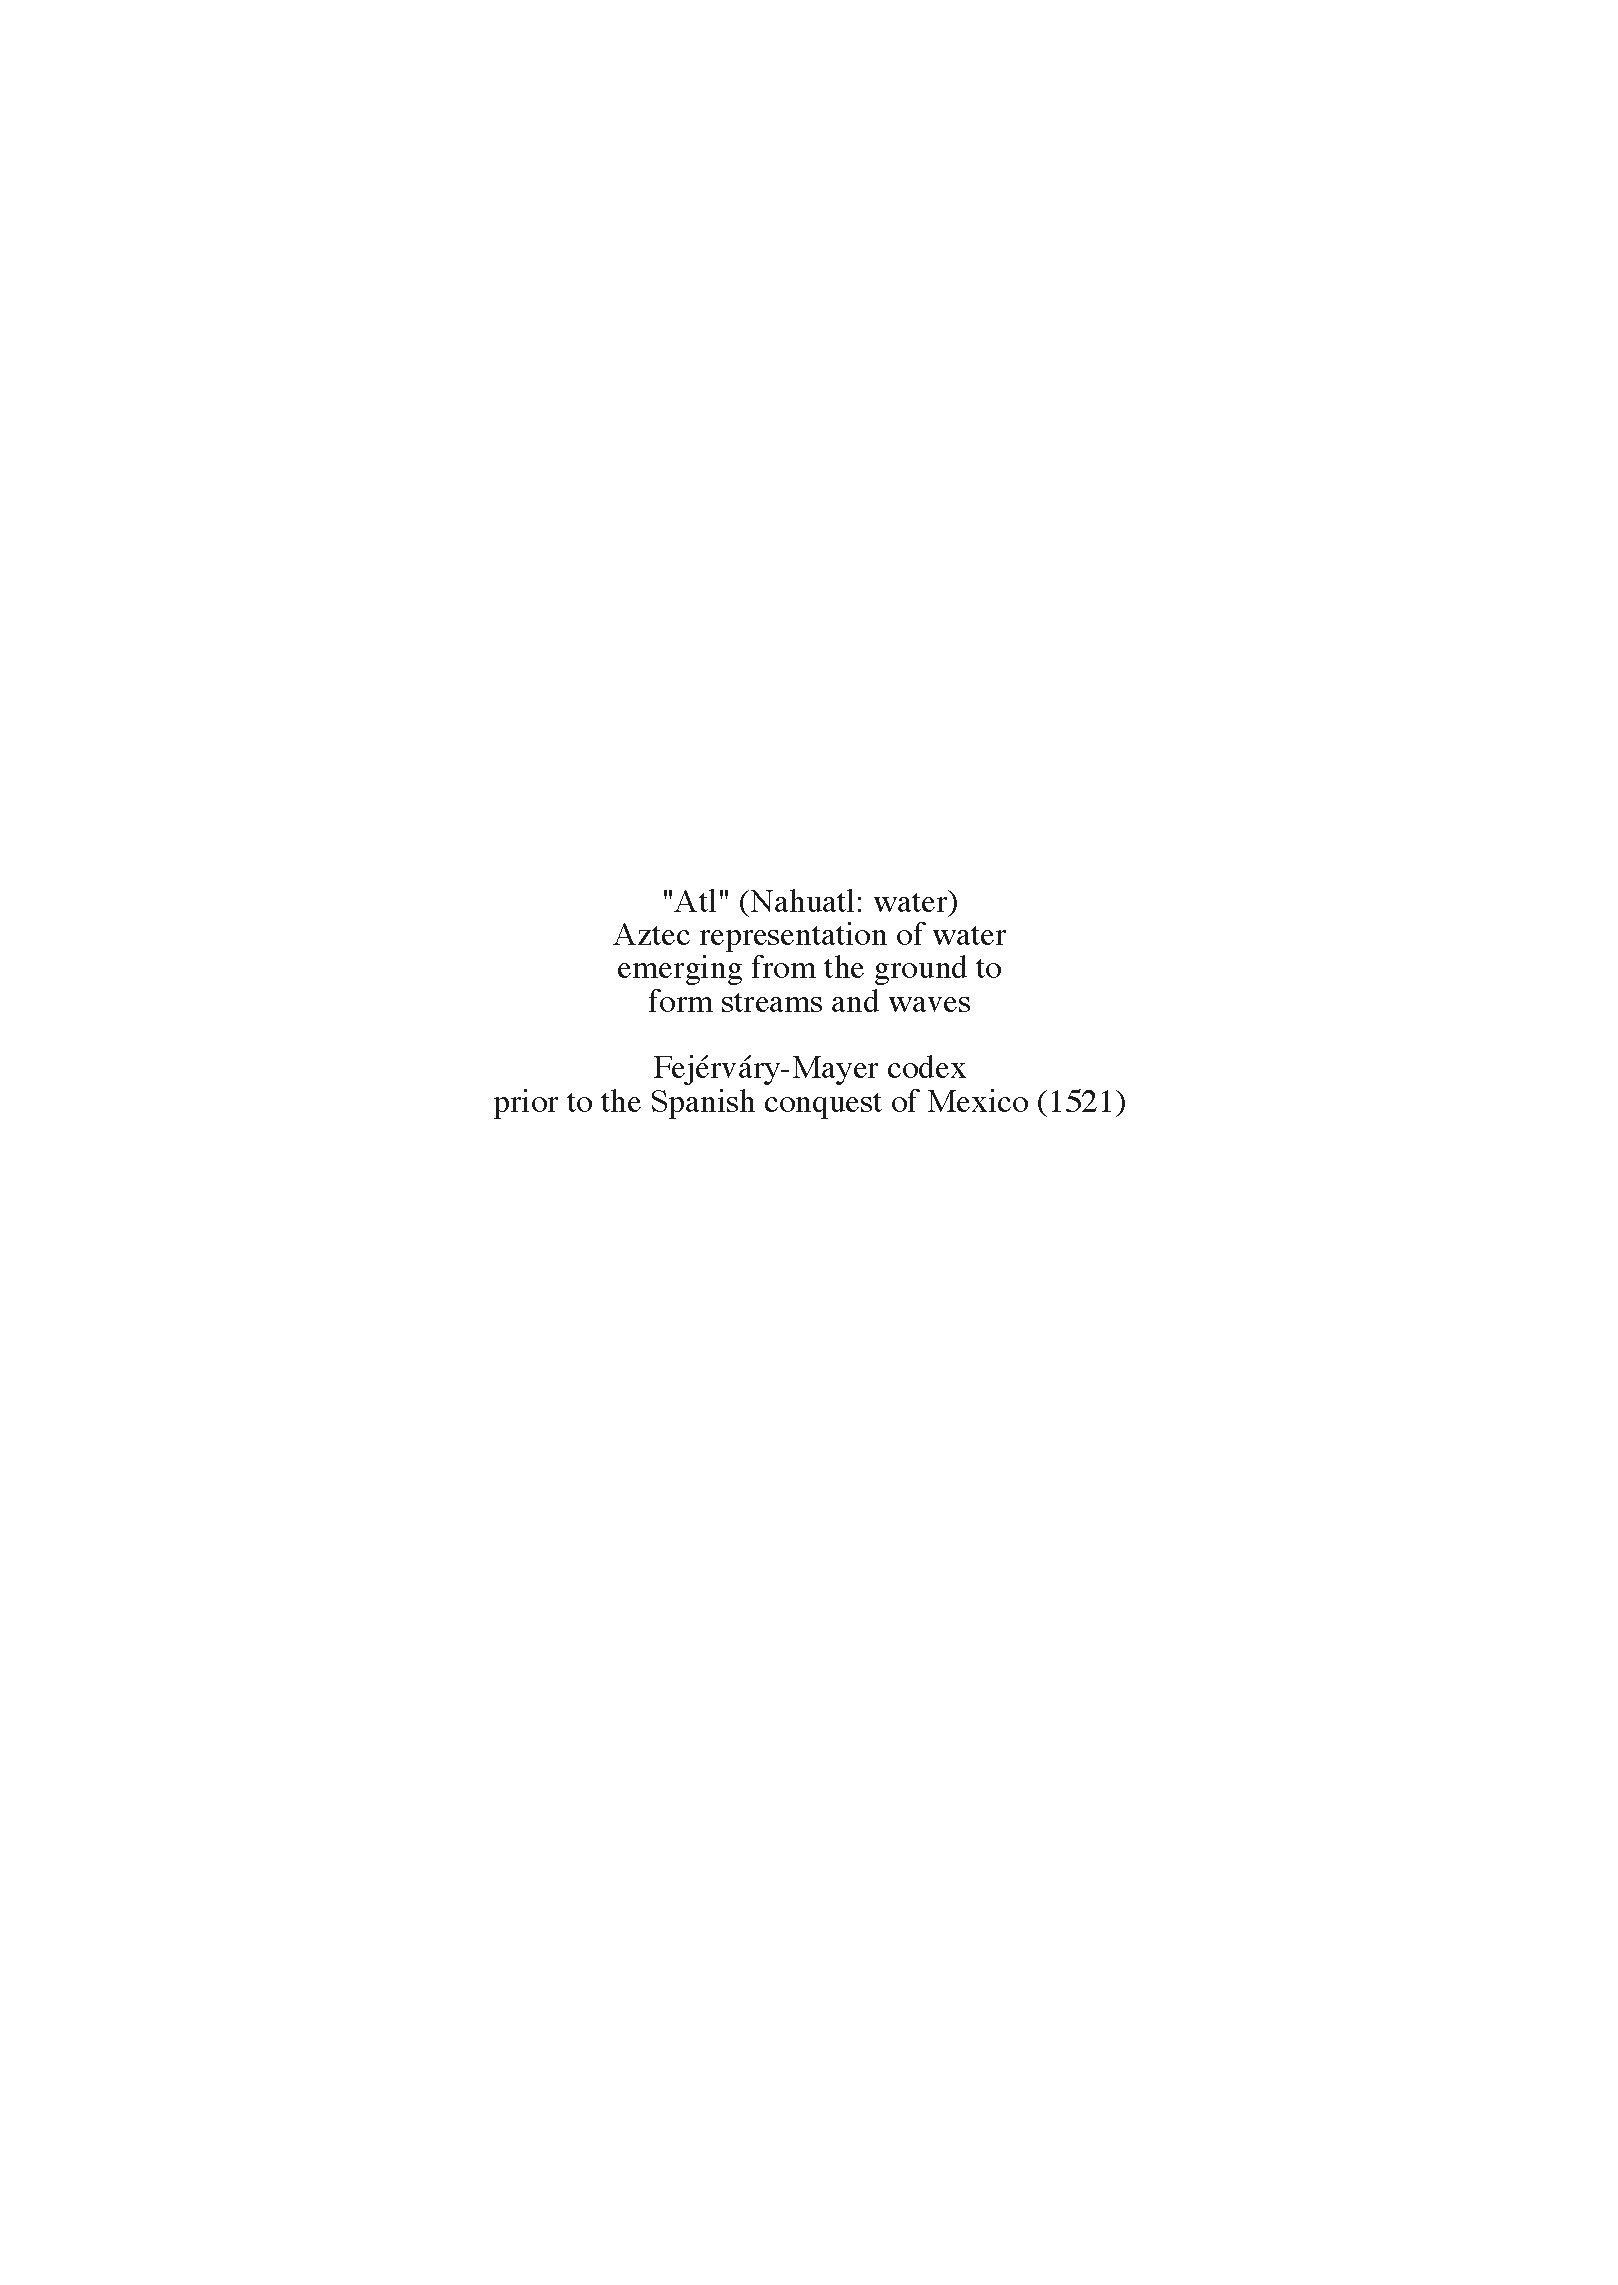
\includegraphics[width=\pdfpagewidth,height=\pdfpageheight]{fullpage_images/CoverBackCaption4Digital.pdf}};
\end{tikzpicture}


\newpage


\begin{tikzpicture}[remember picture,overlay]
\node at (current page.center) {
\includegraphics[width=\pdfpagewidth,height=\pdfpageheight]{fullpage_images/CoverBack4Digital.pdf}};
\end{tikzpicture}


\end{spacing}			

\setstretch{\dnormalspacing}

\end{document}